%% LyX 2.4.3 created this file.  For more info, see https://www.lyx.org/.
%% Do not edit unless you really know what you are doing.
\documentclass[journal,article,submit,moreauthors]{Definitions/mdpi}
\usepackage[utf8]{inputenc}
\synctex=-1
\usepackage{cprotect}
\usepackage{float}
\usepackage{url}
\usepackage{bm}
\usepackage{varwidth}
\usepackage{amstext}
\usepackage{graphicx}

\makeatletter

%%%%%%%%%%%%%%%%%%%%%%%%%%%%%% LyX specific LaTeX commands.

\Title{PEAO: A Cooperative Parallel Enzyme Optimization Algorithm with Adaptive }

\Author{Glykeria Kyrou$^{1}$, Ioannis G. Tsoulos$^{2}$ and Vasileios Charilogis$^{3}$ }


\address{$^{1}$\quad{}Department of Informatics and Telecommunications,
University of Ioannina, 47150 Kostaki Artas, Greece; g.kyrou@uoi.gr\\
$^{2}$\quad{}Department of Informatics and Telecommunications, University
of Ioannina, 47150 Kostaki Artas, Greece; itsoulos@uoi.gr \\
$^{3}$\quad{}Department of Informatics and Telecommunications, University
of Ioannina, 47150 Kostaki Artas, Greece; charilog@uoi.gr}


\corres{Correspondence: g.kyrou@uoi.gr}


\abstract{In recent years, bio-inspired optimization algorithms have been widely
used for solving complex optimization problems. In this paper, we
propose the Parallel Enzyme Action Optimization (PEAO) algorithm,
a parallel bio-inspired optimization algorithm with a multi-strategy
communication mechanism. The algorithm divides the population into
multiple subpopulations that evolve in parallel, enhancing the exploration
capability of the search space. PEAO combines adaptive search factors,
local search procedures and communication mechanisms between subpopulations,
reducing the probability of premature convergence and improving the
quality of the obtained solutions. In addition, clustering techniques
and termination criteria based on similarity and convergence measures
are incorporated to improve efficiency and reduce unnecessary computations.
Experimental results on benchmark functions demonstrate that PEAO
achieves faster convergence, increased robustness and competitive
performance compared to classical optimization methods.}


\keyword{Parallel optimization; Evolutionary techniques; Stochastic methods;
Large-scale problems; Multi-strategy communication}

%% Because html converters don't know tabularnewline
\providecommand{\tabularnewline}{\\}
%% Variable width box for table cells
\newenvironment{cellvarwidth}[1][t]
    {\begin{varwidth}[#1]{\linewidth}}
    {\@finalstrut\@arstrutbox\end{varwidth}}
\floatstyle{ruled}
\newfloat{algorithm}{tbp}{loa}
\providecommand{\algorithmname}{Algorithm}
\floatname{algorithm}{\protect\algorithmname}

%%%%%%%%%%%%%%%%%%%%%%%%%%%%%% User specified LaTeX commands.
%  LaTeX support: latex@mdpi.com 
%  For support, please attach all files needed for compiling as well as the log file, and specify your operating system, LaTeX version, and LaTeX editor.

%=================================================================
%\documentclass[preprints,article,submit,moreauthors]{Definitions/mdpi} 
% For posting an early version of this manuscript as a preprint, you may use "preprints" as the journal. Changing "submit" to "accept" before posting will remove line numbers.

% Below journals will use APA reference format:
% admsci, aieduc, behavsci, businesses, econometrics, economies, education, ejihpe, famsci, games, humans, ijcs, ijfs, investment, fclam, jintelligence, journalmedia, jrfm, jsam, languages, opermanag, peacestud, pmh, psycholint, publications, tourismhosp, youth

% Below journals will use Chicago reference format:
% arts, genealogy, histories, humanities, laws, literature, religions, risks, socsci

%--------------------
% Class Options:
%--------------------
%----------
% journal
%----------
% Choose between the following MDPI journals:
% accountaudit, acn, acoustics, actuators, addictions, addictprev, adhesives, adolescents, aerobiology, aerospace, agriculture, agriengineering, agrochemicals, agronomy, ai, aichem, aieng, aimater, aimed, aipa, air, aisens, aisoc, algorithms, allergies, alloys, amh, analog, analytica, analytics, anatomia, anesthres, animals, antibiotics, antibodies, antioxidants, applbiosci, appliedchem, appliedmath, appliedphys, applmech, applmicrobiol, applnano, applsci, aps, aquacj, archaeolstud, architecture, arm, arthropoda, asc, asi, astronautics, astronomy, atmosphere, atoms, audiolres, automation, axioms, bacteria, batteries, bdcc, beverages, biochem, bioengineering, biologics, biology, biomass, biomechanics, biomed, biomedicines, biomedinformatics, biomimetics, biomolecules, biophysica, bioresourbioprod, biosensors, biosphere, biotech, birds, blockchains, bloods, blsf, brainsci, breath, buildings, cancers, carbon, cardio, cardiogenetics, cardiovascmed, catalysts, cells, ceramics, challenges, chemengineering, chemistry, chemosensors, chemproc, children, chips, cimb, civileng, cleantechnol, climate, clinbioenerg, clinpract, clockssleep, cmd, cmtr, coasts, coatings, colloids, colorants, commodities, complexities, complications, compounds, computation, computers, condensedmatter, conservation, constrmater, cosmetics, covid, crops, cryo, cryptography, crystals, csmf, ctn, culture, curroncol, cyber, dairy, data, ddc, dentistry, dermato, dermatopathology, designs, devices, dhi, diabetology, diagnostics, dietetics, digital, disabilities, diseases, diversity, dna, drones, drugreact, drylands, dynamics, earth, ebj, ecm, ecologies, edm, eesp, electricity, electrochem, electronicmat, electronics, embodiedintell, encyclopedia, endocrines, energies, eng, engproc, entomology, entropy, environments, environremediat, epidemiologia, epigenomes, esa, est, fermentation, fibers, fintech, fire, fishes, fluids, foodeng, foods, forecasting, forensicsci, forests, fossstud, foundations, fractalfract, freshwater, fuels, future, futureinternet, futurepharmacol, futurephys, futuretransp, galaxies, gases, gastroent, gastrointestdisord, gastronomy, gels, genes, geochem, geographies, geohazards, geomatics, geometry, geosciences, geotechnics, geriatrics, germs, glacies, grainsci, grasses, green, greenhealth, gucdd, gynecolcancer, hardware, hazardousmatters, healthcare, healthcmater, hearts, hemato, hematolrep, hep, heritage, higheredu, highthroughput, horticulturae, hospitals, hydrobiology, hydrogen, hydrology, hydrometeorology, hydropower, hygiene, idr, iic, ijem, ijerph, ijgi, ijmd, ijms, ijns, ijom, ijp, ijpb, ijt, ijtm, ijtpp, ijtst, ime, immuno, industries, inflammj, informatics, information, infrastructures, inorganics, insects, instruments, inventions, iot, j, jaestheticmed, jal, japma, jcdd, jcm, jcp, jcrm, jcs, jcto, jdad, jdb, jdream, jemr, jeta, jfb, jfmk, jfth, jgbg, jgg, jimaging, jlpea, jmahp, jmmp, jmms, jmp, jmse, jne, jnt, jof, joi, joitmc, joma, jop, joptm, jor, jox, jpbi, jphytomed, jpm, jsan, jtaer, jvd, jzbg, kidneydial, kinasesphosphatases, knowledge, labmed, laboratories, lam, land, lasers, legumes, life, lights, limnolrev, lipidology, liquids, livers, logics, logistics, lubricants, lymphatics, machines, macromol, magnetism, magnetochemistry, make, marinedrugs, maritime, materials, materproc, mathematics, mca, mcb, measurements, medicina, medicines, medsci, membranes, merits, metabolites, metals, meteorology, methane, metrics, metrology, micro, microarrays, microbiolres, microelectronics, micromachines, microorganisms, microplastics, microwave, minerals, mining, mmphys, modelling, molbank, molecules, mollusca, mps, msf, mti, multimedia, muscles, nanoenergyadv, nanomanufacturing, nanomaterials, ncrna, ndt, network, neuroglia, neuroimaging, neurolint, neurosci, nitrogen, notspecified, nursrep, nutraceuticals, nutrients, obesities, occuphealth, oceans, ohbm, onco, optics, oral, organics, organoids, osteology, oxygen, pandemics, parasites, parasitologia, particles, pathogens, pathophysiology, pediatrrep, pets, pharmaceuticals, pharmaceutics, pharmacoepidemiology, pharmacy, phc, philosophies, photochem, photonics, photovoltaics, phycology, physchem, physics, physiologia, plants, plasma, platforms, pollutants, polymers, polysaccharides, populations, poultry, powders, precision, precisoncol, preprints, proceedings, processes, prosthesis, proteomes, psf, psychiatryint, psychoactives, purification, quantumrep, quaternary, qubs, radiation, rareearths, rdt, reactions, realestate, receptors, recycling, regeneration, remotesensing, reports, reprodmed, resources, rheumato, rjpm, robotics, rsee, ruminants, safety, sanpp, sca, sci, scipharm, sclerosis, seeds, sensors, separations, sexes, shi, signals, sinusitis, siuj, skins, smartcities, smartfish, sna, societies, software, soilsystems, solar, solids, spectroscj, sports, standards, stats, std, stratsediment, stresses, strokerep, superintelligence, surfaces, surgeries, suschem, sustainability, sustainfoods, sustainpackag, symmetry, synbio, systems, tae, targets, taxonomy, technologies, telecom, test, textiles, thalassrep, therapeutics, thermo, timespace, tomography, toxics, toxins, tph, transplantology, transportation, traumacare, traumas, tri, tropicalmed, universe, urbansci, uro, vaccines, vehicles, venereology, vetsci, vibration, virtualworlds, viruses, vision, waste, water, welding, wem, wevj, wild, wind, women, world, zoonoticdis

%---------
% article
%---------
% The default type of manuscript is "article", but can be replaced by: 
% abstract, addendum, article, book, bookreview, briefreport, casereport, comment, commentary, communication, conferenceproceedings, correction, conferencereport, entry, expressionofconcern, extendedabstract, datadescriptor, editorial, essay, erratum, hypothesis, interestingimage, obituary, opinion, projectreport, reply, retraction, review, perspective, protocol, shortnote, studyprotocol, systematicreview, supfile, technicalnote, viewpoint, guidelines, registeredreport, tutorial
% supfile = supplementary materials

%----------
% submit
%----------
% The class option "submit" will be changed to "accept" by the Editorial Office when the paper is accepted. This will only make changes to the frontpage (e.g., the logo of the journal will get visible), the headings, and the copyright information. Also, line numbering will be removed. Journal info and pagination for accepted papers will also be assigned by the Editorial Office.

%------------------
% moreauthors
%------------------
% If there is only one author the class option oneauthor should be used. Otherwise use the class option moreauthors.

%=================================================================
% MDPI internal commands - do not modify
\firstpage{1} 
\setcounter{page}{\@firstpage}
\pubvolume{1}
\issuenum{1}
\articlenumber{0}
\pubyear{2026}
\copyrightyear{2026}
%\externaleditor{Firstname Lastname} % More than 1 editor, please add `` and '' before the last editor name
\datereceived{}
\daterevised{ } % Comment out if no revised date
\dateaccepted{}
\datepublished{}
%\datecorrected{} % For corrected papers include a "Corrected: XXX" date in the original paper.
%\dateretracted{} % For retracted papers include a "RETRACTED: XXX" date in the original paper.
%\doinum{} % Used for some special journals, like molbank
%\pdfoutput=1 % Uncommented for upload to arXiv.org
%\CorrStatement{yes}  % For updates
%\longauthorlist{yes} % For many authors that exceed the left citation part
%\IsAssociation{yes} % For association journals

%=================================================================
% Add packages and commands here. The following packages are loaded in our class file: fontenc, inputenc, calc, indentfirst, fancyhdr, graphicx, epstopdf, lastpage, ifthen, lineno, float, amsmath, setspace, enumitem, mathpazo, booktabs, titlesec, etoolbox, tabto, xcolor, soul, multirow, microtype, tikz, totcount, changepage, attrib, upgreek, cleveref, amsthm, hyphenat, natbib, hyperref, footmisc, url, geometry, newfloat, caption

%=================================================================
%% Please use the following mathematics environments: Theorem, Lemma, Corollary, Proposition, Characterization, Property, Problem, Example, ExamplesandDefinitions, Hypothesis, Remark, Definition, Notation, Assumption
%% For proofs, please use the proof environment (the amsthm package is loaded by the MDPI class).

%=================================================================
% The fields PACS, MSC, and JEL may be left empty or commented out if not applicable
%\PACS{J0101}
%\MSC{}
%\JEL{}

%%%%%%%%%%%%%%%%%%%%%%%%%%%%%%%%%%%%%%%%%%
% Only for the journal Diversity
%\LSID{\url{http://}}

%%%%%%%%%%%%%%%%%%%%%%%%%%%%%%%%%%%%%%%%%%
% Only for the journal Applied Sciences:
%\featuredapplication{Authors are encouraged to provide a concise description of the specific application or a potential application of the work. This section is not mandatory.}
%%%%%%%%%%%%%%%%%%%%%%%%%%%%%%%%%%%%%%%%%%

%%%%%%%%%%%%%%%%%%%%%%%%%%%%%%%%%%%%%%%%%%
% Only for the journal Data:
%\dataset{DOI number or link to the deposited data set in cases where the data set is published or set to be published separately. If the data set is submitted and will be published as a supplement to this paper in the journal Data, this field will be filled by the editors of the journal. In this case, please make sure to submit the data set as a supplement when entering your manuscript into our manuscript editorial system.}

%\datasetlicense{license under which the data set is made available (CC0, CC-BY, CC-BY-SA, CC-BY-NC, etc.)}

%%%%%%%%%%%%%%%%%%%%%%%%%%%%%%%%%%%%%%%%%%
% Only for the journal BioTech, Fishes, Neuroimaging and Toxins
%\keycontribution{The breakthroughs or highlights of the manuscript. Authors can write one or two sentences to describe the most important part of the paper.}

%%%%%%%%%%%%%%%%%%%%%%%%%%%%%%%%%%%%%%%%%%
% Only for the journal Encyclopedia
%\encyclopediadef{Instead of the abstract}
%\entrylink{The Link to this entry published on the encyclopedia platform.}
%%%%%%%%%%%%%%%%%%%%%%%%%%%%%%%%%%%%%%%%%%

%%%%%%%%%%%%%%%%%%%%%%%%%%%%%%%%%%%%%%%%%%
% Different journals have different requirements. Please check the specific journal guidelines in the "Instructions for Authors" on the journal's official website.
 
%\addhighlights{yes}
%\renewcommand{\addhighlights}{%
%
%\noindent This is an optional section, the goal of which is to increase the discoverability and readability of the article via search engines and other scholars. Highlights should not be a copy of the abstract, but a simple overview allowing the reader to quickly and simply find out what the article is about and what can be cited from it. Each of these parts should be up to 2 bullet points.\vspace{3pt}\\
%\textbf{What are the main findings?}
% \begin{itemize}[labelsep=2.5mm,topsep=-3pt]
% \item First bullet.
% \item Second bullet.
% \end{itemize}\vspace{3pt}
%\textbf{What are the implications of the main findings?}
% \begin{itemize}[labelsep=2.5mm,topsep=-3pt]
% \item First bullet.
% \item Second bullet.
% \end{itemize}
%}
%%%%%%%%%%%%%%%%%%%%%%%%%%%%%%%%%%%%%%%%%%

\makeatother

\begin{document}
\maketitle

\section{Introduction}

The\textbf{ }basic goal of global optimization is to find the global
minimum of a continuous multidimensional function, which is defined
as:
\begin{equation}
x^{*}=\mbox{arg}\min_{x\in S}f(x)\label{eq:eq1}
\end{equation}
with $S$: 
\[
S=\left[a_{1},b_{1}\right]\times\left[a_{2},b_{2}\right]\times\ldots\left[a_{n},b_{n}\right]
\]
with $a_{i}$ and $b_{i}$ representing lower and upper bounds for
each variable $x_{i}$.

The continuous increase in the dimensionality and complexity of modern
optimization problems has created a growing demand for optimization
algorithms capable of efficiently exploring large and multimodal search
spaces \citep{DE_Large,Large1,Large2,Large3} while maintaining reasonable
computational requirements. Such challenges often arise in mechanical
design \citep{mechanical design,mechanical design-1} machine learning
\citep{machine_learning_1,machine_learning_2} and data analysis \citep{big data analysis}
where the search landscape often contains many local optima. Although
population-based metaheuristic algorithms have demonstrated significant
success in addressing these problems, their performance often deteriorates
as the dimensionality of the problem increases, leading to slow convergence,
premature stagnation and excessive computational cost. The Enzyme
Action Optimizer (EAO) is a recently introduced bio-inspired optimization
algorithm that models the catalytic behavior of enzymes during biochemical
reactions. Since its introduction by Rodan et al. \citep{EAO-1} EAO
has demonstrated competitive performance across a wide range of benchmark
and real-world optimization problems. Recent studies have successfully
applied EAO to infinite impulse response filter identification problems,
where it exhibited strong convergence characteristics under different
filter configurations \citep{EAO1.}. Furthermore, modified variants
of EAO have been employed for the design of fractional-order PID controllers
in nonlinear continuous stirred tank reactor systems, demonstrating
effective control performance and robustness in challenging dynamic
environments \citep{EAO2.}. Enhanced EAO frameworks have also been
proposed for feature selection in medical data classification tasks,
achieving improved predictive performance through more effective exploration
and diversity preservation mechanisms \citep{EAO3}. In addition to
these applications, EAO has been successfully utilized for the design
of robust two-degree-of-freedom PIDA controllers in magnetic levitation
systems, highlighting its effectiveness in complex control engineering
problems \citep{EAO5}. The algorithm has also been applied to parameter
identification in nonlinear systems, further demonstrating its capability
to handle challenging estimation and modeling tasks \citep{EAO4-1}.
Moreover, recent research has introduced the Dynamic Enzyme Action
Optimizer (DEAO), an adaptive variant of EAO that incorporates dynamic
search mechanisms to improve the balance between exploration and exploitation
and enhance optimization performance on classical benchmark functions
\citep{EAO4}. Collectively, these studies demonstrate the flexibility,
robustness and adaptability of the EAO search mechanism across a diverse
range of optimization applications. Despite these promising developments,
the original EAO and most of its existing variants primarily rely
on single-population search processes. Consequently, they may encounter
difficulties when addressing large-scale and highly multimodal optimization
problems where maintaining population diversity preserving exploration
capability and avoiding premature convergence become increasingly
challenging. In addition, the absence of structured cooperation among
search agents may limit the efficient dissemination of useful search
information throughout the population. Motivated by these limitations,
this work proposes a novel cooperative parallel framework termed Parallel
Enzyme Action Optimizer (PEAO) which extends the original EAO through
distributed population evolution and structured information exchange
mechanisms. The proposed approach introduces a distributed search
architecture based on multiple interacting clusters that evolve concurrently
and cooperate through structured information exchange. Instead of
evolving a single population, the search process is decomposed into
several semi-independent subpopulations that perform exploration simultaneously
while periodically exchanging information through dedicated communication
mechanisms. This cooperative structure aims to improve population
diversity, strengthen global exploration, and reduce the probability
of premature convergence. A key component of the proposed framework
is the introduction of an adaptive propagation mechanism that enables
the controlled dissemination of high-quality solutions among clusters.
By facilitating the transfer of promising search information across
different regions of the population, the propagation process accelerates
convergence while preserving sufficient diversity to maintain exploration
capabilities. Although a recent study introduced a parallel EAO-based
optimizer with a multi-strategy communication mechanism for breast
cancer diagnosis \citep{PEAO}, the present work investigates PEAO
as a general-purpose optimization framework, emphasizing cooperative
cluster evolution, propagation-based information transfer, similarity-based
termination and the systematic study of communication strategies.
Unlike existing EAO variants, the proposed framework combines distributed
search, adaptive propagation, communication-based cooperation, and
similarity-driven convergence monitoring within a unified optimization
architecture.

The main contributions of this work can be summarized as follows:
\begin{itemize}
\item A cooperative parallel extension of the Enzyme Action Optimizer is
proposed, based on the partitioning of the population into multiple
interacting clusters that perform concurrent search operations.
\item A propagation mechanism is introduced to facilitate the exchange of
high-quality solutions among clusters, accelerating convergence while
maintaining population diversity.
\item Multiple communication strategies are incorporated, enabling diverse
forms of information exchange and cooperative interaction among subpopulations.
\item A similarity-based termination criterion is developed to identify
convergence among clusters and reduce redundant computational effort.
\item A scalable optimization framework is developed that improves the balance
between exploration and exploitation and is particularly suitable
for high-dimensional and computationally demanding optimization problems.
\end{itemize}
The remainder of this paper is organized as follows. Section \ref{sec:Materials-and-Methods}
presents the proposed Parallel Enzyme Action Optimizer framework and
its underlying mechanisms. Section \ref{sec:Results} describes the
experimental methodology and benchmark problems. Section \ref{sec:Discussion}
discusses the obtained results and analyzes the influence of the various
algorithmic components. Finally, section \ref{sec:Conclusions} concludes
the paper and outlines future research directions.

\section{Materials and Methods\label{sec:Materials-and-Methods}}

\subsection{\textbf{PEAO Algorithm}}

The proposed Parallel Enzyme Action Optimization (PEAO) is a population-based
metaheuristic optimization algorithm designed to provide an effective
balance between global exploration and local exploitation while enhancing
search diversity through parallel cooperative search. In PEAO, the
population is divided into multiple subpopulations that evolve simultaneously
and independently within the $D$-dimensional search space. Each individual
$x_{i}$ represents a candidate solution of the optimization problem.
Initially, a population of $N$ individuals is randomly generated
within the prescribed search bounds and distributed among the available
subpopulations. The objective function value is then evaluated for
each individual, and the best solution found so far is identified
as $x_{best}$. During the optimization process, an adaptive factor
$A$ is dynamically adjusted to regulate the balance between exploration
and exploitation. This factor gradually modifies the search behavior
of the algorithm, allowing a smooth transition from exploration-oriented
movements to more exploitative search patterns as the optimization
progresses. For each individual, three candidate solutions are generated
through different search mechanisms. The first candidate is produced
using a sinusoidal perturbation strategy guided by the current best
solution. This mechanism introduces nonlinear oscillatory movements
around promising regions of the search space, enhancing the diversification
capability of the algorithm and encouraging the exploration of unexplored
areas. The second and third candidates are generated using Lévy-flight-based
search operators. First, two randomly selected individuals are used
to construct a difference vector, which introduces population-driven
search information. A Lévy random walk is then employed to perturb
the current solution and generate long-distance exploratory moves.
In the second candidate generation mechanism, a Lévy vector and a
vector scaling factor are combined with the difference vector and
the attraction toward the global best solution. This formulation allows
each dimension to evolve independently, thereby increasing the search
diversity and improving the capability of escaping local optima. In
the third candidate generation mechanism, a scalar Lévy step and a
scalar scaling factor are employed. Unlike the previous strategy,
the same perturbation strength is applied to all dimensions, resulting
in a more coherent search movement toward promising regions. The coexistence
of vector-based and scalar-based search operators provides complementary
search behaviors, enabling the algorithm to maintain an effective
balance between diversification and intensification. After generating
the three candidate solutions, their objective function values are
evaluated and the best candidate is selected. A greedy selection mechanism
is then applied, whereby the current solution is replaced only if
the selected candidate exhibits equal or better fitness. This strategy
guarantees that the quality of the population does not deteriorate
during the optimization process. To further enhance local exploitation,
a local search procedure can be activated with probability $p_{l}$.
When triggered, a gradient-based local refinement method such as BFGS
is applied to the current solution. This local improvement phase enables
the algorithm to accelerate convergence and increase solution accuracy,
particularly during the later stages of the optimization process.
At the end of each iteration, all individuals are re-evaluated and
the global best solution is updated. In addition, the algorithm employs
an adaptive termination criterion based on the observed progress of
the optimization process. The search is terminated when no significant
improvement in solution quality is detected and the population has
effectively stabilized. This criterion helps reduce computational
cost by preventing unnecessary objective function evaluations once
convergence has been achieved. By combining sinusoidal perturbation,
Lévy-flight exploration, population-difference learning, adaptive
attraction toward the best solution and optional local search refinement
the proposed PEAO achieves a robust search behavior capable of effectively
handling complex, nonlinear and multimodal optimization problems.
The main steps of the PEAO algorithm are summarized in the following
Algorithm.

{\scriptsize{}
\begin{algorithm}
\caption{The PEAO algorithm \label{alg:original=000391lgorithm}}

{\scriptsize\textbf{INPUT}}{\scriptsize\par}

{\scriptsize - $f$: objective function}{\scriptsize\par}

{\scriptsize - $N$: population size}{\scriptsize\par}

{\scriptsize - $D$: problem dimension}{\scriptsize\par}

{\scriptsize - $T$: maximum number of iterations}{\scriptsize\par}

{\scriptsize - $EC$: enzyme concentration}{\scriptsize\par}

{\scriptsize - $\beta$: Levy parameter}{\scriptsize\par}

{\scriptsize - $N_{t}$: termination criterion}{\scriptsize\par}

{\scriptsize$p_{l}\in[0,1]$ as the local search rate.}{\scriptsize\par}

{\scriptsize\textbf{OUTPUT}}{\scriptsize\par}

{\scriptsize -$x_{best}$: best solution}{\scriptsize\par}

{\scriptsize\textbf{INITIALIZATION}}{\scriptsize\par}

{\scriptsize - }{\scriptsize\textbf{Set $iter\leftarrow0$ }}{\scriptsize as
the iteration counter}{\scriptsize\par}

{\scriptsize\textbf{- Initialize individuals}}{\scriptsize{} $x_{i}\in R^{D},$
$i\in$ \{1..N\}}{\scriptsize\par}

{\scriptsize\textbf{- Compute }}{\scriptsize fitness $F_{i}\leftarrow f(x_{i})$
for each individual}{\scriptsize\par}

{\scriptsize\textbf{- Identify}}{\scriptsize{} best solution: $x_{best}$}{\scriptsize\par}

{\scriptsize\textbf{main pseudocode}}{\scriptsize\par}

{\scriptsize 01}{\scriptsize\textbf{ while }}{\scriptsize stopping criterion
is not met}{\scriptsize\textbf{ do}}{\scriptsize\par}

{\scriptsize 02 \hspace{0.5cm}}{\scriptsize\textbf{Compute}}{\scriptsize{}
adaptive factor: $A\leftarrow\sqrt{\frac{iter}{T}}$}{\scriptsize\par}

{\scriptsize 03 \hspace{0.5cm}}{\scriptsize\textbf{for}}{\scriptsize{}
each individual $i,$ $i\in$ \{1..N\} }{\scriptsize\textbf{do}}{\scriptsize\par}

{\scriptsize 04\hspace{0.5cm}\hspace{0.5cm}}{\scriptsize\textbf{Draw}}{\scriptsize{}
$r$ $\backsim$$U(0,1)$}{\scriptsize\par}

{\scriptsize 05\hspace{0.5cm}\hspace{0.5cm}}{\scriptsize\textbf{Generate}}{\scriptsize{}
Candidate 1: $C_{1}\leftarrow(x_{best}-x_{i}$$)+r\cdot sin(A\cdot x_{i}$
)}{\scriptsize\par}

{\scriptsize 06\hspace{0.5cm}\hspace{0.5cm}}{\scriptsize\textbf{Select
}}{\scriptsize two random individuals $x_{p}$ and $x_{q}$}{\scriptsize\par}

{\scriptsize 07\hspace{0.5cm}\hspace{0.5cm}}{\scriptsize\textbf{Compute}}{\scriptsize{}
difference vector: $DV\leftarrow x_{p}-x_{q}$}{\scriptsize\par}

{\scriptsize 08\hspace{0.5cm}\hspace{0.5cm}}{\scriptsize\textbf{Generate
}}{\scriptsize Levy vector $Lu_{D}($$\beta)\leftarrow Levy\,(D,\beta)$}{\scriptsize\par}

{\scriptsize 09\hspace{0.5cm}\hspace{0.5cm}}{\scriptsize\textbf{Generate}}{\scriptsize{}
Candidate 2A: $C2A\leftarrow x_{i}+Lu_{D}(\beta)\cdot$$DV+A\cdot scA\cdot(x_{best}-x_{i})$
where $scA\in[EC,1]^{D}$}{\scriptsize\par}

{\scriptsize 10\hspace{0.5cm}\hspace{0.5cm}}{\scriptsize\textbf{Generate
}}{\scriptsize Levy scalar $Lu_{1}($$\beta)\leftarrow Levy\,(1,\beta)$}{\scriptsize\par}

{\scriptsize 11\hspace{0.5cm}\hspace{0.5cm}}{\scriptsize\textbf{Generate}}{\scriptsize{}
Candidate 2B: $C2B\leftarrow x_{i}+Lu_{1}(\beta)\cdot DV$$+A\cdot scB\cdot(x_{best}-x_{i})$
where $scB\in[EC,1]$}{\scriptsize\par}

{\scriptsize 12\hspace{0.5cm}\hspace{0.5cm}}{\scriptsize\textbf{Evaluate
}}{\scriptsize$C1,C2A,C2B$}{\scriptsize\par}

{\scriptsize 13\hspace{0.5cm}\hspace{0.5cm}}{\scriptsize\textbf{Select
}}{\scriptsize the best candidate: $C\leftarrow argmin{f(C1),f(C2A),f(C2B)}$}{\scriptsize\par}

{\scriptsize 14\hspace{0.5cm}\hspace{0.5cm}}{\scriptsize\textbf{if}}{\scriptsize{}
$f(C)\leq f(x_{i})$}{\scriptsize\textbf{ then}}{\scriptsize\par}

{\scriptsize 15\hspace{0.5cm}\hspace{0.5cm}\hspace{0.5cm}$x_{i}\leftarrow C$}{\scriptsize\par}

{\scriptsize 16\hspace{0.5cm}\hspace{0.5cm}\hspace{0.5cm}$F_{i}\leftarrow f(C)$}{\scriptsize\par}

{\scriptsize 17\hspace{0.5cm}\hspace{0.5cm}}{\scriptsize\textbf{Endif}}{\scriptsize\par}

{\scriptsize 18\hspace{0.5cm}\hspace{0.5cm}}{\scriptsize\textbf{Draw}}{\scriptsize{}
$r$ $\backsim$$U(0,1)$}{\scriptsize\par}

{\scriptsize 19\hspace{0.5cm}\hspace{0.5cm}}{\scriptsize\textbf{if}}{\scriptsize{}
$r\leq p_{l}$}{\scriptsize\textbf{ then}}{\scriptsize\par}

{\scriptsize 20\hspace{0.5cm}\hspace{0.5cm}\hspace{0.5cm}}{\scriptsize\textbf{Apply
}}{\scriptsize local search $x_{i}\leftarrow LS(x_{i})$\citep{BFGS}}{\scriptsize\par}

{\scriptsize 21\hspace{0.5cm}\hspace{0.5cm}\hspace{0.5cm}$F_{i}\leftarrow f(x_{i})$}{\scriptsize\par}

{\scriptsize 22\hspace{0.5cm}\hspace{0.5cm}}{\scriptsize\textbf{end
if}}{\scriptsize\par}

{\scriptsize 23 \hspace{0.5cm}}{\scriptsize\textbf{endfor}}{\scriptsize\par}

{\scriptsize 24 \hspace{0.5cm}}{\scriptsize\textbf{Set}}{\scriptsize{}
$iter=iter+1$}{\scriptsize\par}

{\scriptsize 25\hspace{0.5cm}}{\scriptsize\textbf{if}}{\scriptsize{}
$iter\geq T$}{\scriptsize\textbf{ then }}{\scriptsize terminate}{\scriptsize\par}

{\scriptsize 26 \hspace{0.5cm}\hspace{0.5cm}}{\scriptsize\textbf{Evaluate
$F_{i}\leftarrow$$f(x_{i})$ }}{\scriptsize for all individuals}{\scriptsize\par}

{\scriptsize 27\hspace{0.5cm}\hspace{0.5cm}}{\scriptsize\textbf{Update
}}{\scriptsize$x_{best}$ based on best fitness value}{\scriptsize\par}

{\scriptsize 28\hspace{0.5cm}\hspace{0.5cm}}{\scriptsize\textbf{Compute
$\delta^{(k)}=|f_{i}^{(iter)}-{\displaystyle f_{i}^{(iter-1)}|}$}}{\scriptsize\citep{stopping_rule}}{\scriptsize\par}

{\scriptsize 29\hspace{0.5cm}\hspace{0.5cm}}{\scriptsize\textbf{if
$\delta^{(k)}\leq\epsilon$ for }}{\scriptsize$N_{t}$iterations }{\scriptsize\textbf{then
}}{\scriptsize terminate.}{\scriptsize\par}

{\scriptsize 30 \hspace{0.5cm}\hspace{0.5cm}\hspace{0.5cm}}{\scriptsize\textbf{Update
}}{\scriptsize$x_{best}$ based on best fitness value}{\scriptsize\par}

{\scriptsize 31}{\scriptsize\textbf{ end while}}{\scriptsize{} // Goto
termination check}{\scriptsize\par}

{\scriptsize Return$x_{best}$}{\scriptsize\par}
\end{algorithm}
}{\scriptsize\par}

\subsection{\textbf{Proposed PEAO Framework}}

\begin{algorithm}[H]
{\scriptsize INPUT}{\scriptsize\par}

{\scriptsize$-f:$ objective function}{\scriptsize\par}

{\scriptsize$-K:$ number of subpopulations}{\scriptsize\par}

{\scriptsize$-C_{R}:$ communication threshold}{\scriptsize\par}

{\scriptsize$-C_{S}:$ communication strategy mode,}{\scriptsize\par}

{\scriptsize$-C_{S}\in{0,1,2,3})$}{\scriptsize\par}

{\scriptsize$-N_{M}:$ propagation method}{\scriptsize\par}

{\scriptsize$-N_{R}:$ propagation rate}{\scriptsize\par}

{\scriptsize$-N_{P}:$ number of propagation agents}{\scriptsize\par}

{\scriptsize$-$$N_{I}$: termination criterion}{\scriptsize\par}

{\scriptsize\textbf{OUTPUT}}{\scriptsize\par}

{\scriptsize$(x_{best}):$ global best solution}{\scriptsize\par}

{\scriptsize\textbf{INITIALIZATION}}{\scriptsize\par}

{\scriptsize$Set\:\:t\leftarrow0$}{\scriptsize\par}

{\scriptsize\textbf{Initialize}}{\scriptsize{} population}{\scriptsize\par}

{\scriptsize\textbf{Divide}}{\scriptsize{} population into $K$ subpopulations}{\scriptsize\par}

{\scriptsize\textbf{Compute}}{\scriptsize{} fitness values}{\scriptsize\par}

{\scriptsize\textbf{Identify}}{\scriptsize{} local best and worst individuals}{\scriptsize\par}

{\scriptsize\textbf{Identify}}{\scriptsize{} global best solution $x_{best}$}{\scriptsize\par}

{\scriptsize\textbf{MAIN PSEUDOCODE}}{\scriptsize\par}

{\scriptsize 01}{\scriptsize\textbf{ while}}{\scriptsize{} stopping criterion
is not met }{\scriptsize\textbf{do}}{\scriptsize\par}

{\scriptsize 02\hspace{0.5cm}}{\scriptsize\textbf{Set}}{\scriptsize{}
$t\leftarrow t+1$}{\scriptsize\par}

{\scriptsize 03\hspace{0.5cm}f}{\scriptsize\textbf{or}}{\scriptsize{}
each subpopulation $k\in{1..K}$in parallel }{\scriptsize\textbf{do}}{\scriptsize\par}

{\scriptsize 04\hspace{0.5cm}\hspace{0.5cm}}{\scriptsize\textbf{Execute}}{\scriptsize{}
one iteration of the Algorithm 1}{\scriptsize\par}

{\scriptsize 05\hspace{0.5cm}\hspace{0.5cm}}{\scriptsize\textbf{Update}}{\scriptsize{}
local best and worst individuals}{\scriptsize\par}

{\scriptsize 06\hspace{0.5cm}\hspace{0.5cm}}{\scriptsize\textbf{if}}{\scriptsize{}
$N_{R}>0$and $t\bmod N_{R}=0$ }{\scriptsize\textbf{then}}{\scriptsize\par}

{\scriptsize 07\hspace{0.5cm}\hspace{0.5cm}\hspace{0.5cm}}{\scriptsize\textbf{Apply}}{\scriptsize{}
propagation scheme $N_{M}$ with $N_{P}$ agents}{\scriptsize\par}

{\scriptsize 08\hspace{0.5cm}\hspace{0.5cm}}{\scriptsize\textbf{endif}}{\scriptsize\par}

{\scriptsize 09\hspace{0.5cm}}{\scriptsize\textbf{endfor}}{\scriptsize\par}

{\scriptsize 10\hspace{0.5cm}}{\scriptsize\textbf{Update}}{\scriptsize{}
global best solution $x_{best}$}{\scriptsize\par}

{\scriptsize 11\hspace{0.5cm}}{\scriptsize\textbf{if }}{\scriptsize$C_{R}>0$
and $t\bmod C_{R}=0$}{\scriptsize\textbf{ then}}{\scriptsize\par}

{\scriptsize 12\hspace{0.5cm}\hspace{0.5cm}}{\scriptsize\textbf{if}}{\scriptsize{}
$C_{S}=0$ }{\scriptsize\textbf{then}}{\scriptsize\par}

{\scriptsize 13\hspace{0.5cm}\hspace{0.5cm}\hspace{0.5cm}$c\leftarrow$
random integer $\in{1,2,3}$}{\scriptsize\par}

{\scriptsize 14\hspace{0.5cm}\hspace{0.5cm}}{\scriptsize\textbf{else}}{\scriptsize\par}

{\scriptsize 15\hspace{0.5cm}\hspace{0.5cm}\hspace{0.5cm}$c\leftarrow C_{S}$}{\scriptsize\par}

{\scriptsize 16\hspace{0.5cm}\hspace{0.5cm}}{\scriptsize\textbf{endif}}{\scriptsize\par}

{\scriptsize 17\hspace{0.5cm}\hspace{0.5cm}}{\scriptsize\textbf{if}}{\scriptsize{}
$c=1$ }{\scriptsize\textbf{then}}{\scriptsize\par}

{\scriptsize 18\hspace{0.5cm}\hspace{0.5cm}\hspace{0.5cm}}{\scriptsize\textbf{Apply}}{\scriptsize{}
Optimal Replacement Strategy}{\scriptsize\par}

{\scriptsize 19\hspace{0.5cm}\hspace{0.5cm}}{\scriptsize\textbf{elseif}}{\scriptsize{}
$c=2$ }{\scriptsize\textbf{then}}{\scriptsize\par}

{\scriptsize 20\hspace{0.5cm}\hspace{0.5cm}\hspace{0.5cm}}{\scriptsize\textbf{Apply
}}{\scriptsize Optimal Mean Replacement Strategy}{\scriptsize\par}

{\scriptsize 21\hspace{0.5cm}\hspace{0.5cm}}{\scriptsize\textbf{else}}{\scriptsize\par}

{\scriptsize 22\hspace{0.5cm}\hspace{0.5cm}\hspace{0.5cm}}{\scriptsize\textbf{Apply}}{\scriptsize{}
Circular Optimal Replacement Strategy}{\scriptsize\par}

{\scriptsize 23\hspace{0.5cm}\hspace{0.5cm}}{\scriptsize\textbf{endif}}{\scriptsize\par}

{\scriptsize 24\hspace{0.5cm}\hspace{0.5cm}\hspace{0.5cm}}{\scriptsize\textbf{Update}}{\scriptsize{}
local best and worst individuals}{\scriptsize\par}

{\scriptsize 25\hspace{0.5cm}\hspace{0.5cm}\hspace{0.5cm}}{\scriptsize\textbf{Update}}{\scriptsize{}
global best solution $x_{best}$}{\scriptsize\par}

{\scriptsize 26 }{\scriptsize\textbf{end while}}{\scriptsize\par}

{\scriptsize\textbf{Return }}{\scriptsize$x_{best}$}{\scriptsize\par}
\end{algorithm}

Furthermore, the steps of the proposed method are also graphically
shown in Figure \ref{fig:Algorithm}.

\begin{figure}

\includegraphics[scale=0.45]{PEAO_final}\caption{Flowchart of the proposed PEAO framework.\label{fig:Algorithm}}
\end{figure}

Figure \ref{fig:Thread-creation-diagram} presents the parallel execution
architecture and communication mechanisms of the proposed PEAO framework.
Each Processing Unit (PU) is responsible for the evolution of a single
subpopulation, within which the core PEAO search procedure is executed
independently. Candidate solutions are generated using the $C1,C2A$
and $C2B$ update mechanisms, while the most promising candidate is
selected through a greedy replacement strategy. The subpopulations
evolve simultaneously and independently, enabling the parallel exploration
of different regions of the search space and promoting population
diversity. After each search cycle, the overall best solution is updated
and the communication condition among subpopulations is evaluated.
When communication is activated, one of the available information-exchange
strategies is applied, namely Optimal Replacement, Optimal Mean Replacement,
or Circular Optimal Replacement. These strategies facilitate the transfer
of useful search knowledge among subpopulations by replacing low-quality
solutions with high-quality information obtained from other search
groups. In addition, the propagation mechanism supports the controlled
dissemination of promising solutions across processing units, enabling
effective cooperation among subpopulations while preserving their
exploration capabilities. The combination of parallel exploration,
controlled information propagation and multi-strategy communication
contributes to maintaining population diversity, accelerating convergence
and strengthening the balance between exploration and exploitation.
As a result, the proposed PEAO framework achieves improved search
efficiency and robustness when solving complex optimization problems.

\begin{figure}

\includegraphics[scale=0.6]{diagram}

\caption{Communication and propagation strategies among subpopulations.\label{fig:Thread-creation-diagram}}
\end{figure}


\subsection{Propagation Mechanism}

The propagation mechanism enables information exchange among subpopulations
by transferring high-quality solutions during the optimization process.
Specifically, the best individual of a subpopulation is propagated
to other subpopulations, replacing their worst-performing individual.
This process enhances cooperation and accelerates convergence toward
promising regions of the search space. To maintain low communication
overhead and scalability, the proposed framework adopts simplified
propagation strategies instead of conventional migration topologies.
Four propagation scenarios are considered:
\begin{itemize}
\item One-to-One (1to1): A randomly selected subpopulation sends its best
solution to another randomly selected subpopulation.
\item One-to-All (1toN): A randomly selected subpopulation propagates its
best solution to all other subpopulations.
\item All-to-One (Nto1): The best solutions of all subpopulations are propagated
to a single randomly selected subpopulation.
\item All-to-All (NtoN): Each subpopulation exchanges its best solution
with all other subpopulations.
\end{itemize}
These strategies promote the dissemination of high-quality solutions
while preserving the computational efficiency of the parallel framework.

\section{Experiments\label{sec:Results} }

This section begins with a description of the functions that will
be used in the experiments and then presents in detail the experiments
that were performed, in which the parameters available in the proposed
algorithm were studied, in order to study their reliability and adequacy. 

\subsection{Test Functions}

A variety of benchmark test functions were used in the conducted experiments.
These functions have been widely adopted in previous studies \citep{test_function,test_function-1,test_function2,test_function3}.
In the present work, the test functions are evaluated using dimensionalities
ranging from 25 to 150, where the constant n denotes the dimension
of the objective function. The benchmark test functions used in the
experimental study are summarized in Table \ref{tab:Benchmark-test-functions}
including their mathematical formulation dimensionality and global
optimum values.
\begin{center}
{\tiny{}
\begin{table}[H]
\centering{}\caption{Benchmark test functions used in experimental study.\label{tab:Benchmark-test-functions}}
{\scriptsize{}%
\begin{tabular}{|c|c|c|c|c|}
\hline 
{\scriptsize\textbf{NAME}} & {\scriptsize\textbf{FORMULA}} & {\scriptsize\textbf{DIM}} & {\scriptsize\textbf{BOUNDS}} & {\scriptsize$G_{min}$}\tabularnewline
\hline 
\hline 
\begin{cellvarwidth}[t]
\centering
{\scriptsize ATTRACTIVE}{\scriptsize\par}

{\scriptsize SECTOR}
\end{cellvarwidth} & {\tiny$f(x)=\left(\sum_{i=1}^{n}(s_{i}x_{i})^{2}\right)^{0.9}$} & {\scriptsize$n$} & {\scriptsize$[-5,5]^{n}$} & {\scriptsize 0}\tabularnewline
\hline 
{\scriptsize BUCHE RASTRIGIN} & {\tiny$f(\mathbf{x})=\sum_{i=1}^{n}\left[z_{i}\cdot\left(1+0.1\cdot\sin(10\pi z_{i})\right)\right]$} & {\scriptsize$n$} & {\scriptsize$[-5.12,5.12]^{n}$} & {\scriptsize 0}\tabularnewline
\hline 
{\scriptsize DIFFERENT POWERS} & {\tiny$f(\mathbf{x})=\sqrt{\sum_{i=1}^{n}|x_{i}|^{2+4\frac{i-1}{n-1}}}$} & {\scriptsize$n$} & {\scriptsize$[-5,5]^{n}$} & {\scriptsize 0}\tabularnewline
\hline 
{\scriptsize DISCUS} & {\tiny$f(x)=10^{6}x_{1}^{2}+\sum_{i=2}^{n}x_{i}^{2}$} & {\scriptsize$n$} & {\scriptsize\textbf{$[-5,5]^{n}$}} & {\scriptsize 0}\tabularnewline
\hline 
{\scriptsize ELLIPSOIDAL} & {\tiny$f(x)=\sum_{i=1}^{n}\left(10^{6}\right)^{\frac{i-1}{n-1}}x_{i}^{2}$} & {\scriptsize$n$} & {\scriptsize$[-5.12,5.12]^{n}$} & {\scriptsize 0}\tabularnewline
\hline 
{\scriptsize GALLAGHER101} & {\tiny$f(\mathbf{x})=\max_{i=1}^{101}\left[h_{i}-w_{i}\sqrt{\sum_{j=1}^{n}(x_{j}-c_{ij})^{2}}\right]$$\ min=101$} & {\scriptsize$n$} & {\scriptsize$[-5,5]^{n}$} & {\scriptsize 0}\tabularnewline
\hline 
{\scriptsize GALLAGHER21} & {\tiny$f(\mathbf{x})=\max_{i=1}^{21}\left[h_{i}-w_{i}\sqrt{\sum_{j=1}^{n}(x_{j}-c_{ij})^{2}}\right]$$\ min=21$} & {\scriptsize$n$} & {\scriptsize$[-5,5]^{n}$} & {\scriptsize 0}\tabularnewline
\hline 
\begin{cellvarwidth}[t]
\centering
{\scriptsize GRIEWANK}{\scriptsize\par}

{\scriptsize ROSENBROCK}
\end{cellvarwidth} & {\tiny$f(\mathbf{x})=\underbrace{\left(\frac{\|\mathbf{x}\|^{2}}{4000}-\prod_{i=1}^{n}\cos\left(\frac{x_{i}}{\sqrt{i}}\right)+1\right)}_{\text{Griewank}}\cdot\underbrace{\left(\frac{1}{10}\sum_{i=1}^{n-1}\left[100(x_{i+1}-x_{i}^{2})^{2}+(1-x_{i})^{2}\right]\right)}_{\text{Rosenbrock}}$} & {\scriptsize$n$} & {\scriptsize$[-5,5]^{n}$} & {\scriptsize 0}\tabularnewline
\hline 
{\scriptsize GRIEWANK} & {\tiny$f(x)=1+\frac{1}{200}\sum_{i=1}^{n}x_{i}^{2}-\prod_{i=1}^{n}\frac{\cos(x_{i})}{\sqrt{(i)}}$} & {\scriptsize$n$} & {\scriptsize$[-100,100]^{n}$} & {\scriptsize 0}\tabularnewline
\hline 
{\scriptsize RASTRIGIN} & {\tiny$f(\mathbf{x})=An+\sum_{i=1}^{n}\left[x_{i}^{2}-A\cos(2\pi x_{i})\right]$$\ A=10$} & {\scriptsize$n$} & {\scriptsize$[-5.12,5.12]^{n}$} & {\scriptsize 0}\tabularnewline
\hline 
{\scriptsize ROSENBROCK} & {\tiny$f(x)=\sum_{i=1}^{n-1}\left(100\left(x_{i+1}-x_{i}^{2}\right)^{2}+\left(x_{i}-1\right)^{2}\right),\quad-30\le x_{i}\le30$} & {\scriptsize$n$} & {\scriptsize$[-30,30]^{n}$} & {\scriptsize 0}\tabularnewline
\hline 
{\scriptsize SHARP RIDGE} & {\tiny$f(\mathbf{x})=x_{1}^{2}+\alpha\sum_{i=2}^{n}x_{i}^{2},\ a>1$} & {\scriptsize$n$} & {\scriptsize$[-5,5]^{n}$} & {\scriptsize 0}\tabularnewline
\hline 
{\scriptsize STEP ELLIPSOIDAL} & {\tiny$f(\mathbf{x})=\sum_{i=1}^{n}\left\lfloor x_{i}+0.5\right\rfloor ^{2}+\alpha\sum_{i=1}^{n}\left(10^{6}\cdot\frac{i-1}{n-1}\right)x_{i}^{2},\ a=1$} & {\scriptsize$n$} & {\scriptsize$[-5,5]^{n}$} & {\scriptsize 0}\tabularnewline
\hline 
{\scriptsize ZAKHAROV} & {\tiny$f(\mathbf{x})=\sum_{i=1}^{n}x_{i}^{2}+\left(\sum_{i=1}^{n}\frac{i}{2}x_{i}\right)^{2}+\left(\sum_{i=1}^{n}\frac{i}{2}x_{i}\right)^{4}$} & {\scriptsize$n$} & {\scriptsize$[-5,10]^{n}$} & {\scriptsize 0}\tabularnewline
\hline 
\end{tabular}}
\end{table}
}{\tiny\par}
\par\end{center}

\subsection{Experimental results }

A series of experiments were carried out for the previously mentioned
functions and these experiments were executed on an AMD RYZEN 5950X
with 128GB RAM. The operating system of the running machine was Debian
Linux. Each experiment was conducted 30 times, with different random
numbers each time, and the averages were recorded. The software used
in the experiments was coded in  C++ using the freely available optimization
environment of OPTIMUS \citep{OPTIMUS} which can be downloaded from\textbf{
}\url{https://github.com/itsoulos/OPTIMUS} (accessed on 23 June 2026).
The adoption of the publicly available OPTIMUS optimization framework
improves the reproducibility of the experimental study and facilitates
independent verification of the reported results by other researchers.
All comparative methods were independently implemented and evaluated
within the same experimental framework and were not directly adopted
from the corresponding literature. All algorithms were implemented
in C++ and executed under identical hardware and software conditions
to ensure a fair and consistent comparison. Specifically, the number
of agents (population size) was set to 200 for all algorithms, the
maximum number of iterations was fixed at 200, and the local search
rate was uniformly set to 5\% (local search probability). These shared
settings ensure that performance differences arise from algorithmic
design rather than differences in experimental configuration. Algorithm
specific parameters were selected according to standard practices
reported in the literature and were kept constant throughout all experiments.
No problem specific parameter tuning was applied in order to avoid
bias and to maintain methodological consistency. The values used for
each parameter are shown in Table \ref{tab:settings}.

\cprotect\paragraph{
\begin{table}[H]
\protect\caption{The values for the experimental parameters.\label{tab:settings}}

\protect\centering{}{\footnotesize{}%
\begin{tabular}{|c|c|c|}
\hline 
{\footnotesize PARAMETER} & {\footnotesize VALUE} & {\footnotesize EXPLANATION}\tabularnewline
\hline 
\hline 
{\footnotesize$N$} & {\footnotesize 200} & {\footnotesize Number of individuals}\tabularnewline
\hline 
{\footnotesize$iter_{max}$} & {\footnotesize 200} & \begin{cellvarwidth}[t]
\centering
{\footnotesize Maximum number of }\protect \\
{\footnotesize iterations}
\end{cellvarwidth}\tabularnewline
\hline 
{\footnotesize$K$} & {\footnotesize 1,3,10,20,30} & {\footnotesize Number of subpopulations}\tabularnewline
\hline 
{\footnotesize$SR$} & {\footnotesize$\delta_{k}^{(iter)}=\left|f_{k,min}^{(iter)}-f_{k,min}^{(iter-1)}\right|$} & {\footnotesize Stopping rule: Similarity}\tabularnewline
\hline 
{\footnotesize$P_{L}$} & {\footnotesize 0.05 (5\%)} & {\footnotesize Local search rate}\tabularnewline
\hline 
\begin{cellvarwidth}[t]
\centering
\begin{description}
\item [{$N_{M}$}]~
\end{description}
\end{cellvarwidth} & {\footnotesize 1to1, 1toN, Nto1, NtoN} & {\footnotesize Propagation method}\tabularnewline
\hline 
\begin{cellvarwidth}[t]
\centering
\begin{description}
\item [{$N_{R}$}]~
\end{description}
\end{cellvarwidth} & {\footnotesize 1,2,3,4...$\le N$} & \begin{cellvarwidth}[t]
\centering
{\footnotesize Number of iterations }\protect \\
{\footnotesize for propagation}
\end{cellvarwidth}\tabularnewline
\hline 
\begin{cellvarwidth}[t]
\centering
\begin{description}
\item [{$N_{P}$}]~
\end{description}
\end{cellvarwidth} & {\footnotesize 1,2,3,4...$\le N$} & \begin{cellvarwidth}[t]
\centering
{\footnotesize Number of agents }\protect \\
{\footnotesize for propagation}
\end{cellvarwidth}\tabularnewline
\hline 
\begin{cellvarwidth}[t]
\centering
\begin{description}
\item [{$N_{T}$}]~
\end{description}
\end{cellvarwidth} & {\footnotesize 1,2,3,4...$\le N$} & \begin{cellvarwidth}[t]
\centering
{\footnotesize Number of subpopulations }\protect \\
{\footnotesize required to satisfy the stopping criterion}
\end{cellvarwidth}\tabularnewline
\hline 
{\footnotesize$F$} & {\footnotesize 0.8} & {\footnotesize Differential weight for DE}\tabularnewline
\hline 
{\footnotesize$CR$} & {\footnotesize 0.9} & {\footnotesize Crossover probability}\tabularnewline
\hline 
{\footnotesize$N_{I}$} & {\footnotesize 8} & {\footnotesize Number of iterations used in the termination rule}\tabularnewline
\hline 
{\footnotesize -} & {\footnotesize 0.05 (5\%)} & {\footnotesize Mutation rate for GA}\tabularnewline
\hline 
{\footnotesize -} & {\footnotesize 0.05 (5\%)} & {\footnotesize Selection Rate for GA}\tabularnewline
\hline 
{\footnotesize -} & {\footnotesize Roulette} & {\footnotesize Selection method for GA}\tabularnewline
\hline 
\end{tabular}}{\footnotesize\par}\protect
\end{table}
}

In the following tables, the reported values correspond to the average
number of function evaluations over 30 independent runs. The values
in parentheses denote the proportion of runs in which the global minimum
was successfully identified. The absence of such values indicates
a success rate of 100\%.

\subsection{Impact of the Number of Clusters}

Table\textbf{ }\ref{tab:3.3 Impact of the Number of Clusters} presents
the comparison of the average number of objective function evaluations
obtained for different numbers of subpopulations (5, 10, 20 and 30
clusters) across benchmark functions of dimensions 25, 50, 100 and
150. Lower values indicate higher computational efficiency. The results
show that the number of clusters has a substantial impact on the performance
of the proposed PEAO algorithm. In most benchmark functions, configurations
with 10 and 20 clusters consistently achieve the lowest numbers of
function evaluations. For example in Zakharov\_100 the number of evaluations
decreases from 8384 with 5 clusters to 4803 and 4718 for 10 and 20
clusters respectively while increasing to 6847 when 30 clusters are
used. Similarly, in Sharp Ridge\_150 the corresponding values are
reduced from 6699 to 5640 and further to 4850 for 10 and 20 clusters
respectively but rise again to 5930 with 30 clusters. These results
indicate that dividing the population into a moderate number of cooperating
subpopulations improves the balance between exploration and exploitation,
allowing the algorithm to locate promising regions of the search space
more efficiently. However, increasing the number of clusters beyond
a certain point may lead to excessive fragmentation of the population
reducing information exchange among subpopulations and consequently
increasing the computational effort required to reach convergence.

In contrast, configurations with only 5 clusters generally require
a larger number of evaluations due to the reduced diversity of the
search process while the use of 30 clusters often leads to performance
degradation. This behavior can be attributed to excessive population
fragmentation which reduces the number of individuals available within
each subpopulation and weakens local exploitation capabilities. As
a result information becomes more dispersed and the search process
less effective in refining high-quality solutions.

The overall computational cost further supports these observations.
The total number of objective function evaluations decreases from
385,708 for 5 clusters to 297,299 for 10 clusters and reaches its
minimum value of 286,096 for 20 clusters. Increasing the number of
clusters to 30 results in a higher computational cost of 351,709 evaluations.
Therefore, the results suggest that configurations with 10--20 clusters
provide the most effective population decomposition strategy achieving
superior search efficiency while maintaining adequate diversity and
convergence stability.

{\scriptsize{}
\begin{table}[H]
{\scriptsize\caption{Comparison of different numbers of subpopulations in terms of average
objective function evaluations. \label{tab:3.3 Impact of the Number of Clusters}}
}{\scriptsize\par}

{\footnotesize{}%
\begin{tabular}{|c|c|c|c|c|}
\hline 
{\footnotesize\textbf{FUNCTION}} & {\footnotesize\textbf{5 CLUSTER}} & {\footnotesize\textbf{10 CLUSTER}} & {\footnotesize\textbf{20 CLUSTER}} & {\footnotesize\textbf{30 CLUSTER}}\tabularnewline
\hline 
\hline 
\begin{cellvarwidth}[t]
\centering
{\footnotesize ATTRACTIVE}{\footnotesize\par}

{\footnotesize SECTOR\_25}
\end{cellvarwidth} & 4796 & 4701 & 4681 & 4749\tabularnewline
\hline 
\begin{cellvarwidth}[t]
\centering
{\footnotesize ATTRACTIVE}{\footnotesize\par}

{\footnotesize SECTOR\_50}
\end{cellvarwidth} & 4958 & 4873 & 4737 & 4803\tabularnewline
\hline 
\begin{cellvarwidth}[t]
\centering
{\footnotesize ATTRACTIVE}{\footnotesize\par}

{\footnotesize SECTOR\_100}
\end{cellvarwidth} & 5104 & 4964 & 4757 & 4813\tabularnewline
\hline 
\begin{cellvarwidth}[t]
\centering
{\footnotesize ATTRACTIVE}{\footnotesize\par}

{\footnotesize SECTOR\_150}
\end{cellvarwidth} & 4979 & 4927 & 4750 & 4805\tabularnewline
\hline 
{\footnotesize BUCHE RASTRIGIN\_25} & 6298 & 4866 & 4807 & 5917\tabularnewline
\hline 
{\footnotesize BUCHE RASTRIGIN\_50} & 8368 & 5874 & 5679 & 7336\tabularnewline
\hline 
{\footnotesize BUCHE RASTRIGIN\_100} & 10352 & 6429 & 6188 & 9071\tabularnewline
\hline 
{\footnotesize BUCHE RASTRIGIN\_150} & 10585 & 4715 & 5934 & 9771\tabularnewline
\hline 
{\footnotesize DISCUS\_25} & 4847 & 4905 & 4687 & 4801\tabularnewline
\hline 
{\footnotesize DISCUS\_50} & 5031 & 4994 & 4777 & 4871\tabularnewline
\hline 
{\footnotesize DISCUS\_100} & 5198 & 5083 & 4806 & 4891\tabularnewline
\hline 
{\footnotesize DISCUS\_150} & 5066 & 4818 & 4789 & 4844\tabularnewline
\hline 
{\footnotesize DIFFERENTPOWERS\_25} & 6688 & 5575 & 4706 & 6204\tabularnewline
\hline 
{\footnotesize DIFFERENTPOWERS\_50} & 8919 & 6784 & 4900 & 6803\tabularnewline
\hline 
{\footnotesize DIFFERENTPOWERS\_100} & 11752 & 5957 & 4702 & 7611\tabularnewline
\hline 
{\footnotesize DIFFERENTPOWERS\_150} & 11616 & 5911 & 4809 & 8720\tabularnewline
\hline 
{\footnotesize ELLIPSOIDAL\_25} & 5352 & 4773 & 4749 & 5229\tabularnewline
\hline 
{\footnotesize ELLIPSOIDAL\_50} & 6513 & 5595 & 5387 & 6339\tabularnewline
\hline 
{\footnotesize ELLIPSOIDAL\_100} & 9340 & 7303 & 6708 & 9017\tabularnewline
\hline 
{\footnotesize ELLIPSOIDAL\_150} & 9934 & 7541 & 7927 & 8680\tabularnewline
\hline 
{\footnotesize GALLAGHER21\_25} & 5629 & 4773 & 4752 & 4876\tabularnewline
\hline 
{\footnotesize GALLAGHER21\_50} & 5652 & 5277 & 5105 & 5133\tabularnewline
\hline 
{\footnotesize GALLAGHER21\_100} & 5587 & 5305 & 5287 & 5515(0.93)\tabularnewline
\hline 
{\footnotesize GALLAGHER21\_150} & 5633 & 5298 & 5225(0.97) & 5175\tabularnewline
\hline 
{\footnotesize GALLAGHER101\_25} & 4960 & 4767 & 4741 & 4865\tabularnewline
\hline 
{\footnotesize GALLAGHER101\_50} & 5617 & 5238 & 5117 & 5180\tabularnewline
\hline 
{\footnotesize GALLAGHER101\_100} & 6165 & 5452 & 5322 & 5527\tabularnewline
\hline 
{\footnotesize GALLAGHER101\_150} & 5650 & 5217 & 5063 & 5439\tabularnewline
\hline 
{\footnotesize GRIEWANK \_25} & 6115 & 4833 & 5157 & 5730\tabularnewline
\hline 
{\footnotesize GRIEWANK \_50} & 6018 & 5557 & 5332 & 5689\tabularnewline
\hline 
{\footnotesize GRIEWANK \_100} & 6470 & 6246 & 5924 & 6260\tabularnewline
\hline 
{\footnotesize GRIEWANK \_150} & 6277 & 5820 & 5741 & 6121\tabularnewline
\hline 
{\footnotesize GRIEWANK\_ROSENBROCK\_25} & 6691 & 4754 & 4821 & 6412\tabularnewline
\hline 
{\footnotesize GRIEWANK\_ROSENBROCK\_50} & 7877 & 5299 & 5147 & 7378\tabularnewline
\hline 
{\footnotesize GRIEWANK\_ROSENBROCK\_100} & 8150 & 5536 & 5659 & 7814\tabularnewline
\hline 
{\footnotesize GRIEWANK\_ROSENBROCK\_150} & 7614 & 5287 & 5500 & 7883\tabularnewline
\hline 
{\footnotesize ROSENBROCK\_25} & 6822 & 4728 & 4686 & 6202\tabularnewline
\hline 
{\footnotesize ROSENBROCK\_50} & 8421 & 5083 & 4779 & 7659\tabularnewline
\hline 
{\footnotesize ROSENBROCK\_100} & 12122 & 5145 & 4814 & 8734\tabularnewline
\hline 
{\footnotesize ROSENBROCK\_150} & 11149 & 4958 & 4773 & 9992\tabularnewline
\hline 
{\footnotesize RARSTIGIN\_25} & 5998 & 4869 & 4756 & 5631\tabularnewline
\hline 
{\footnotesize RARSTIGIN\_50} & 7074 & 5675 & 5352 & 6433\tabularnewline
\hline 
{\footnotesize RARSTIGIN\_100} & 7851 & 5999 & 5862 & 7425\tabularnewline
\hline 
{\footnotesize RARSTIGIN\_150} & 7507 & 5686 & 5641 & 7129\tabularnewline
\hline 
{\footnotesize STEP ELLIPSOIDAL\_25} & 4670 & 4669 & 4669 & 4670\tabularnewline
\hline 
{\footnotesize STEP ELLIPSOIDAL\_50} & 4699 & 4699 & 4697 & 4698\tabularnewline
\hline 
{\footnotesize STEP ELLIPSOIDAL\_100} & 4701 & 4701 & 4701 & 4702\tabularnewline
\hline 
{\footnotesize STEP ELLIPSOIDAL\_150} & 4696 & 4695 & 4697 & 4696\tabularnewline
\hline 
{\footnotesize SHARP RIDGE\_25} & 6158 & 4795 & 4713 & 6099\tabularnewline
\hline 
{\footnotesize SHARP RIDGE\_50} & 6707 & 5338 & 4835 & 5898\tabularnewline
\hline 
{\footnotesize SHARP RIDGE\_100} & 7153 & 5644 & 4793 & 6017\tabularnewline
\hline 
{\footnotesize SHARP RIDGE\_150} & 6699 & 5640 & 4850 & 5930\tabularnewline
\hline 
{\footnotesize ZAKHAROV\_25} & 5312 & 4827 & 4721 & 5092\tabularnewline
\hline 
{\footnotesize ZAKHAROV\_50} & 6350 & 5179 & 4770 & 5756\tabularnewline
\hline 
{\footnotesize ZAKHAROV\_100} & 8384 & 4803 & 4718 & 6847\tabularnewline
\hline 
{\footnotesize ZAKHAROV\_150} & 7434 & 4919 & 4896 & 7827\tabularnewline
\hline 
 & 385708 & 297299 & 286096(0.99) & 351709(0.99)\tabularnewline
\hline 
\end{tabular}}{\footnotesize\par}
\end{table}
}{\scriptsize\par}

\begin{figure}
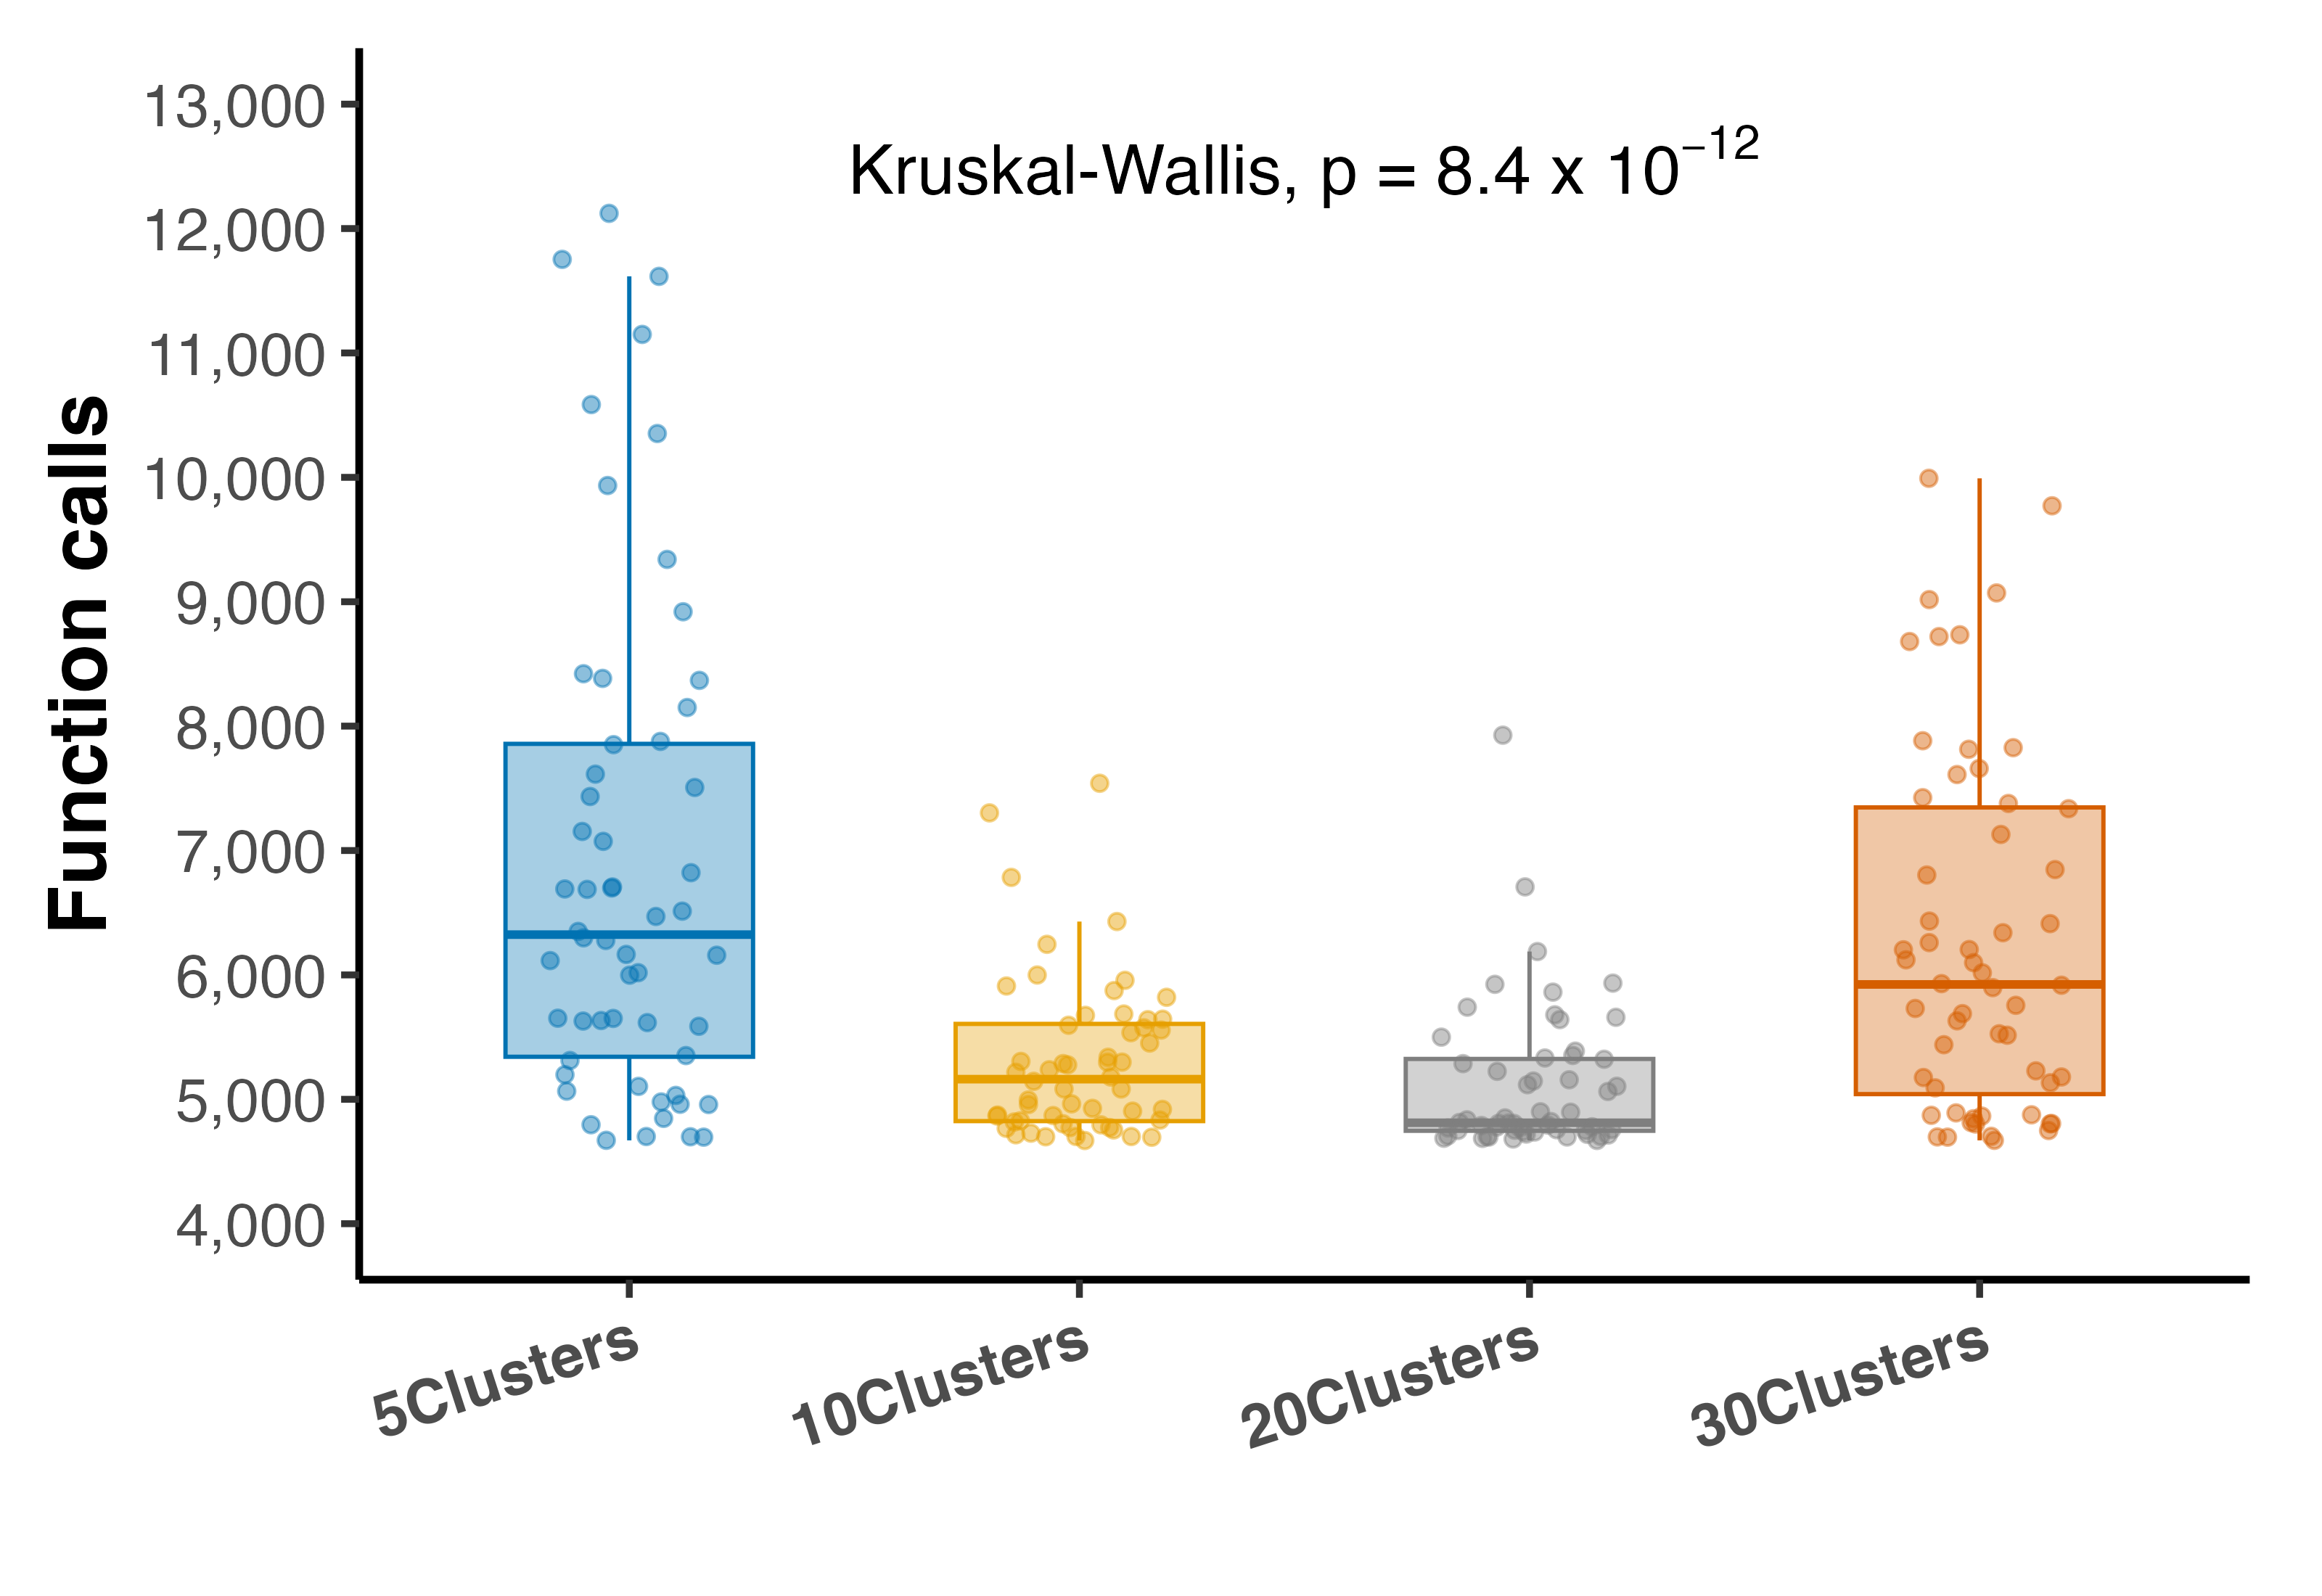
\includegraphics[scale=0.6]{clusters}

\caption{Impact of the Number of Clusters.\label{fig:Impact-of-the}}
\end{figure}

Figure\textbf{ }\ref{fig:Impact-of-the} presents the influence of
the number of clusters on the computational efficiency of the proposed
algorithm. The results reveal that the configurations employing 10
and 20 clusters require significantly fewer function evaluations than
the alternatives while also demonstrating lower variability across
independent runs. Conversely, the 5-clusters configuration exhibits
the highest median number of function calls and substantial dispersion,
indicating slower and less reliable convergence. Although the 30-cluster
configuration performs better than the 5-cluster case its variability
remains considerably higher than that observed for 10 and 20 clusters.
The Kruskal--Wallis test ($p=8.4\times10{{}^-}^{{{}^1}{{}^2}}$)
indicates statistically significant differences among the examined
configurations. These findings suggest that using a moderate number
of clusters can substantially enhance the search efficiency and robustness
of the algorithm, with 10 and 20 clusters yielding the most favorable
performance.

\subsection{Impact of Propagation Mechanism}

Table\textbf{ }\ref{tab:3.4 Impact of Propagation Mechanism}\textbf{
}presents the comparative analysis of the proposed PEAO algorithm
with and without the propagation mechanism (PROP = 1 and PROP = 0)
in terms of average objective function evaluations across benchmark
functions of dimensions 25, 50, 100 and 150. Lower values indicate
improved computational efficiency. The results clearly demonstrate
that the propagation mechanism constitutes a fundamental component
of the proposed framework, leading to substantial reductions in the
number of objective function evaluations for almost all benchmark
problems. More specifically, the benefits of propagation become particularly
evident in complex multimodal functions. For example, in Büche Rastrigin\_150
the number of evaluations decreases from 135,523 without propagation
to only 4,715 when propagation is enabled. Similar improvements are
observed in Sharp Ridge\_150 where the evaluations are reduced from
21,109 to 5,640 and in Zakharov\_150 where the computational cost
decreases from 28,647 to 4,919 evaluations. Comparable behavior is
also observed across lower-dimensional instances indicating that the
effectiveness of propagation is independent of problem size. The observed
improvement can be attributed to the efficient exchange of information
among clusters. Through propagation promising solutions discovered
in one cluster become available to the remaining clusters accelerating
convergence and reducing redundant exploration of already-investigated
regions of the search space. Consequently, the algorithm is able to
exploit high-quality regions more effectively while maintaining adequate
search diversity. The overall computational cost further highlights
the importance of the propagation mechanism. The total number of objective
function evaluations decreases dramatically from 1,897,933 in the
case without propagation (PROP = 0) to only 297,299 when propagation
is enabled (PROP = 1) corresponding to a reduction of more than 84\%
in the required computational effort. Such a significant improvement
confirms that information propagation substantially enhances the search
efficiency of the proposed cooperative framework. Overall, the results
demonstrate that the integration of propagation is essential for the
successful operation of PEAO. By facilitating cooperation among clusters
and accelerating the dissemination of high-quality information throughout
the population, the propagation mechanism significantly reduces computational
cost and improves the overall efficiency and scalability of the algorithm.

{\scriptsize{}
\begin{table}[H]
{\scriptsize\caption{Comparison of the proposed method with and without propagation mechanism
in terms of average objective function evaluations.\label{tab:3.4 Impact of Propagation Mechanism}}
}{\scriptsize\par}
\centering{}{\small{}%
\begin{tabular}{|c|c|c|}
\hline 
{\small\textbf{FUNCTION}} & {\small\textbf{PROP=0}} & {\small\textbf{PROP=1}}\tabularnewline
\hline 
\hline 
\begin{cellvarwidth}[t]
\centering
{\small ATTRACTIVE}{\small\par}

{\small SECTOR\_25}
\end{cellvarwidth} & 6582 & {\small 4701}\tabularnewline
\hline 
\begin{cellvarwidth}[t]
\centering
{\small ATTRACTIVE}{\small\par}

{\small SECTOR\_50}
\end{cellvarwidth} & 6817 & {\small 4873}\tabularnewline
\hline 
\begin{cellvarwidth}[t]
\centering
{\small ATTRACTIVE}{\small\par}

{\small SECTOR\_100}
\end{cellvarwidth} & 7088 & {\small 4964}\tabularnewline
\hline 
\begin{cellvarwidth}[t]
\centering
{\small ATTRACTIVE}{\small\par}

{\small SECTOR\_150}
\end{cellvarwidth} & 6970 & {\small 4927}\tabularnewline
\hline 
{\small BUCHE RASTRIGIN\_25} & 58030 & {\small 4866}\tabularnewline
\hline 
{\small BUCHE RASTRIGIN\_50} & 86188 & {\small 5874}\tabularnewline
\hline 
{\small BUCHE RASTRIGIN\_100} & 116211 & {\small 6429}\tabularnewline
\hline 
{\small BUCHE RASTRIGIN\_150} & 135523 & {\small 4715}\tabularnewline
\hline 
{\small DISCUS\_25} & 7111 & {\small 4905}\tabularnewline
\hline 
{\small DISCUS\_50} & 7268 & {\small 4994}\tabularnewline
\hline 
{\small DISCUS\_100} & 7668 & {\small 5083}\tabularnewline
\hline 
{\small DISCUS\_150} & 7428 & {\small 4818}\tabularnewline
\hline 
{\small DIFFERENTPOWERS\_25} & 24052 & {\small 5575}\tabularnewline
\hline 
{\small DIFFERENTPOWERS\_50} & 32492 & {\small 6784}\tabularnewline
\hline 
{\small DIFFERENTPOWERS\_100} & 47065 & {\small 5957}\tabularnewline
\hline 
{\small DIFFERENTPOWERS\_150} & 52426 & {\small 5911}\tabularnewline
\hline 
{\small ELLIPSOIDAL\_25} & 11246 & {\small 4773}\tabularnewline
\hline 
{\small ELLIPSOIDAL\_50} & 18284 & {\small 5595}\tabularnewline
\hline 
{\small ELLIPSOIDAL\_100} & 30864 & {\small 7303}\tabularnewline
\hline 
{\small ELLIPSOIDAL\_150} & 39305 & {\small 7541}\tabularnewline
\hline 
{\small GALLAGHER21\_25} & 46411 & {\small 4773}\tabularnewline
\hline 
{\small GALLAGHER21\_50} & 13166 & {\small 5277}\tabularnewline
\hline 
{\small GALLAGHER21\_100} & 24696 & {\small 5305}\tabularnewline
\hline 
{\small GALLAGHER21\_150} & 12226(0.83) & {\small 5298}\tabularnewline
\hline 
{\small GALLAGHER101\_25} & 69639 & {\small 4767}\tabularnewline
\hline 
{\small GALLAGHER101\_50} & 81366 & {\small 5238}\tabularnewline
\hline 
{\small GALLAGHER101\_100} & 70335 & {\small 5452}\tabularnewline
\hline 
{\small GALLAGHER101\_150} & 55891 & {\small 5217}\tabularnewline
\hline 
{\small GRIEWANK \_25} & 16507 & {\small 4833}\tabularnewline
\hline 
{\small GRIEWANK \_50} & 10253 & {\small 5557}\tabularnewline
\hline 
{\small GRIEWANK \_100} & 10034 & {\small 6246}\tabularnewline
\hline 
{\small GRIEWANK \_150} & 9414 & {\small 5820}\tabularnewline
\hline 
{\small GRIEWANK\_ROSENBROCK\_25} & 24232 & {\small 4754}\tabularnewline
\hline 
{\small GRIEWANK\_ROSENBROCK\_50} & 28600 & {\small 5299}\tabularnewline
\hline 
{\small GRIEWANK\_ROSENBROCK\_100} & 33069 & {\small 5536}\tabularnewline
\hline 
{\small GRIEWANK\_ROSENBROCK\_150} & 34478 & {\small 5287}\tabularnewline
\hline 
{\small ROSENBROCK\_25} & 22919 & {\small 4728}\tabularnewline
\hline 
{\small ROSENBROCK\_50} & 34647 & {\small 5083}\tabularnewline
\hline 
{\small ROSENBROCK\_100} & 54081 & {\small 5145}\tabularnewline
\hline 
{\small ROSENBROCK\_150} & 69505 & {\small 4958}\tabularnewline
\hline 
{\small RARSTIGIN\_25} & 51593 & {\small 4869}\tabularnewline
\hline 
{\small RARSTIGIN\_50} & 62684 & {\small 5675}\tabularnewline
\hline 
{\small RARSTIGIN\_100} & 69952 & {\small 5999}\tabularnewline
\hline 
{\small RARSTIGIN\_150} & 66543 & {\small 5686}\tabularnewline
\hline 
{\small STEP ELLIPSOIDAL\_25} & 16205 & {\small 4669}\tabularnewline
\hline 
{\small STEP ELLIPSOIDAL\_50} & 14935 & {\small 4699}\tabularnewline
\hline 
{\small STEP ELLIPSOIDAL\_100} & 14030 & {\small 4701}\tabularnewline
\hline 
{\small STEP ELLIPSOIDAL\_150} & 13747 & {\small 4695}\tabularnewline
\hline 
{\small SHARP RIDGE\_25} & 18646 & {\small 4795}\tabularnewline
\hline 
{\small SHARP RIDGE\_50} & 19932 & {\small 5338}\tabularnewline
\hline 
{\small SHARP RIDGE\_100} & 20959 & {\small 5644}\tabularnewline
\hline 
{\small SHARP RIDGE\_150} & 21109 & {\small 5640}\tabularnewline
\hline 
{\small ZAKHAROV\_25} & 10499 & {\small 4827}\tabularnewline
\hline 
{\small ZAKHAROV\_50} & 15031 & {\small 5179}\tabularnewline
\hline 
{\small ZAKHAROV\_100} & 23334 & {\small 4803}\tabularnewline
\hline 
{\small ZAKHAROV\_150} & 28647 & {\small 4919}\tabularnewline
\hline 
 & 1897933(0.99) & {\small 297299}\tabularnewline
\hline 
\end{tabular}}{\small\par}
\end{table}
}{\scriptsize\par}

\begin{figure}
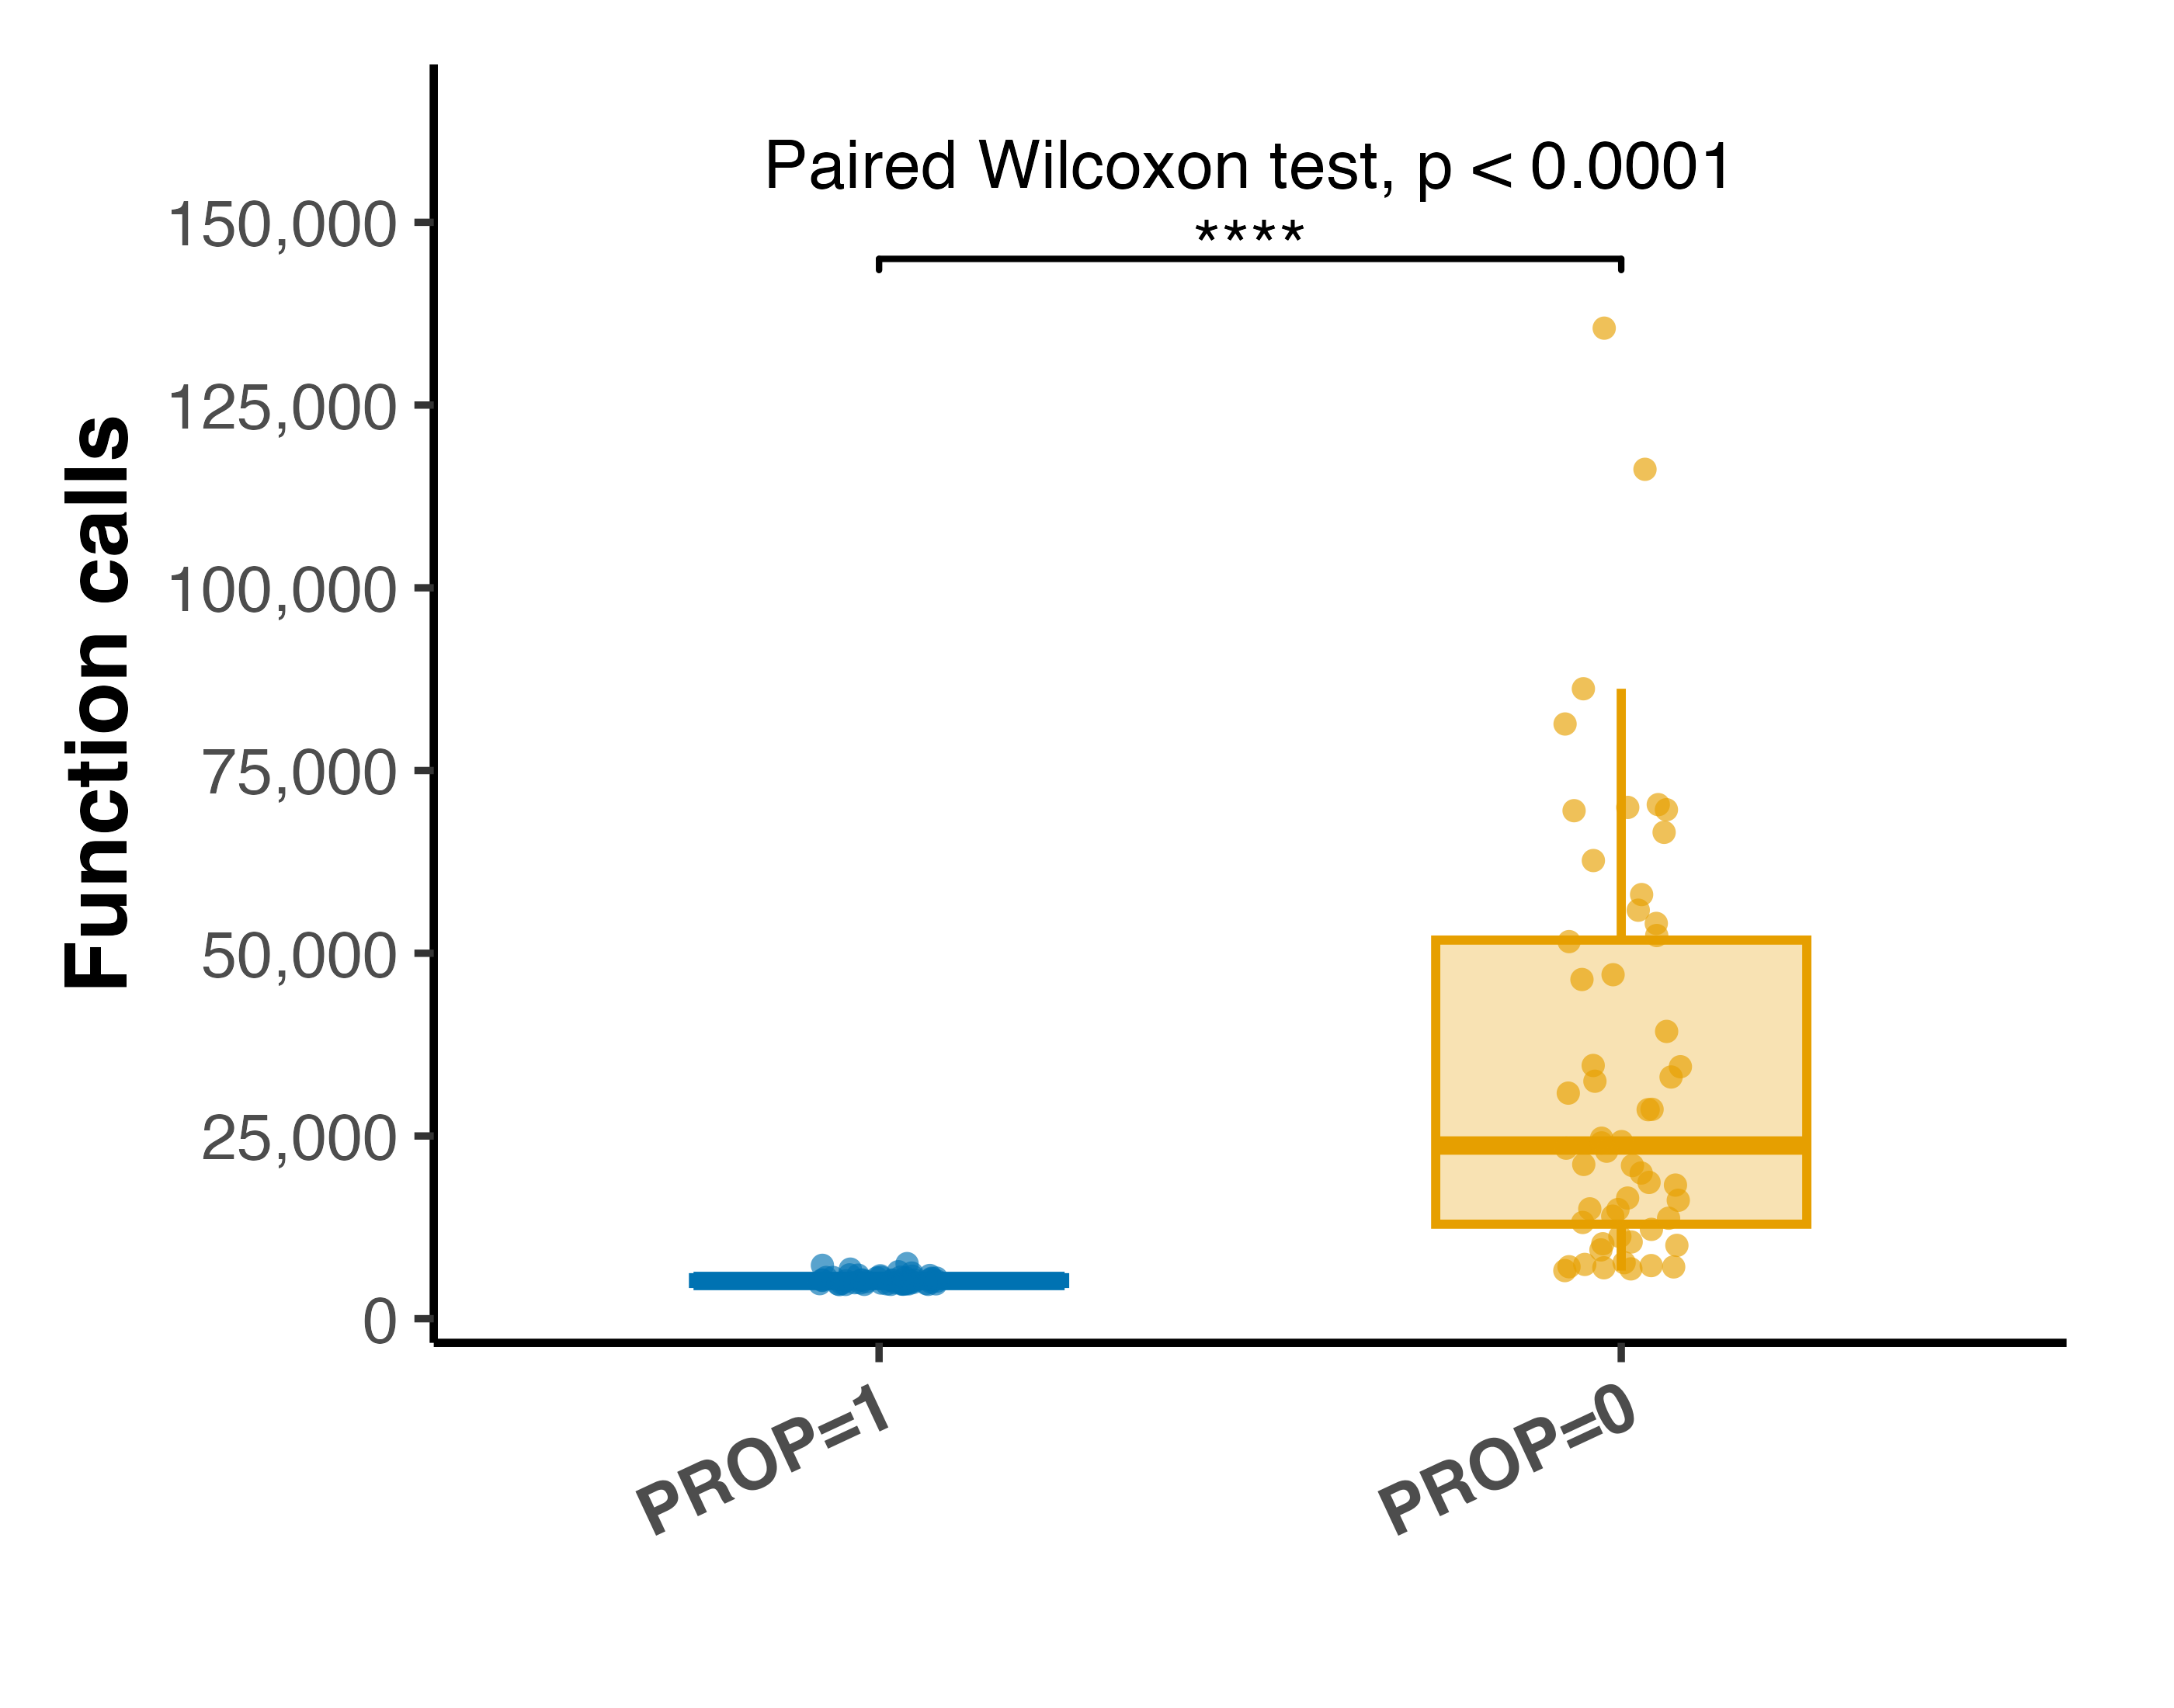
\includegraphics[scale=0.6]{prop_0_or_1}

\caption{Impact of Propagation Mechanism. \label{fig:Impact-of-Propagation}}
\end{figure}

Figure\textbf{ }\ref{fig:Impact-of-Propagation} presents the effect
of the propagation mechanism on the performance of the proposed method.
In particular PROP = 1 corresponds to the configuration where propagation
is enabled, whereas PROP = 0 denotes the configuration without propagation.
The comparison is based on the total number of function calls required
by the algorithm across all experimental runs. As illustrated in the
figure enabling propagation leads to a substantial reduction in the
number of function evaluations. The distribution of results for PROP
= 1 is concentrated around significantly lower values and exhibits
considerably lower variability compared to the PROP = 0 configuration.
In contrast, when propagation is disabled the algorithm requires a
much larger number of function calls and demonstrates greater dispersion
indicating slower and less stable convergence behavior. To assess
the statistical significance of this difference, a paired Wilcoxon
signed-rank test was performed. According to the conventional significance
notation (ns: p \textgreater{} 0.05, {*}: p \textless{} 0.05, {*}{*}:
p \textless{} 0.01, {*}{*}{*}: p \textless{} 0.001, {*}{*}{*}{*}:
p \textless{} 0.0001) where the overall result (p \textless{} 0.0001)
indicates a highly significant difference between the two configurations.
Therefore, the experimental evidence strongly suggests that the propagation
mechanism contributes substantially to improving the convergence efficiency
of the proposed method. Although the propagation mechanism introduces
an additional communication cost due to the exchange of information
among agents this overhead is not directly reflected in the reported
number of function evaluations. Nevertheless, the communication burden
remains relatively small as only a limited set of high-quality candidate
solutions is propagated during the optimization process. Consequently,
the additional communication cost is largely compensated by the significant
reduction in computational effort and the faster convergence achieved
when propagation is enabled. These findings demonstrate that the benefits
of propagation clearly outweigh its associated overhead and highlight
its importance within the proposed optimization framework.

\subsection{Impact of Communication Strategies with 10 Subpopulations}

Table\textbf{ }\ref{tab:3.5 Communication Strategy with 10 Subpopulations}\textbf{
}presents the average number of objective function evaluations obtained
by four different communication strategies (1to1, 1toN, Nto1 and NtoN)
when the optimization process is performed using 10 subpopulations.
Lower values correspond to better performance. The results clearly
indicate that the NtoN communication strategy consistently achieves
the lowest number of function evaluations across the majority of the
benchmark problems. In the Attractive Sector functions, NtoN requires
between 4701 and 4964 function calls, whereas the corresponding values
for the 1to1 strategy range from 6083 to 6320. Similar behavior is
observed for the Discus and Step Ellipsoidal functions where NtoN
consistently outperforms all other communication schemes. The superiority
of the NtoN strategy becomes even more pronounced for more challenging
optimization problems. For example, in Büche Rastrigin\_150 the NtoN
strategy requires only 4715 function evaluations compared to 48431,
14223 and 17452 for the 1to1, 1toN and Nto1 strategies respectively.
Likewise, for Zakharov\_150 NtoN achieves convergence with 4919 evaluations
whereas the corresponding values are 21919, 8894 and 10539 for 1to1,
1toN and Nto1. Similar improvements can be observed in the Rosenbrock,
Rastrigin and Sharp Ridge functions demonstrating the robustness of
the NtoN communication scheme across different problem characteristics.
The overall computational cost further supports this observation.
The total number of function evaluations accumulated over all benchmark
problems is 982,812 for the 1to1 strategy 446,500 for 1toN 518,590
for Nto1 and only 297,299 for NtoN. Consequently, the NtoN strategy
reduces the overall computational effort by approximately 70\% compared
to 1to1 33\% compared to 1toN and 43\% compared to Nto1. These findings
suggest that allowing all subpopulations to simultaneously exchange
information significantly enhances cooperation among search agents
and accelerates the dissemination of high-quality solutions throughout
the population. As a result, the NtoN communication mechanism achieves
faster convergence and lower computational requirements than the alternative
propagation strategies making it the most effective communication
scheme for the considered configuration with 10 subpopulations.

{\scriptsize{}
\begin{table}[H]
{\scriptsize\caption{Comparison of propagation strategies under 10 subpopulations in terms
of average objective function evaluations.\label{tab:3.5 Communication Strategy with 10 Subpopulations}}
}{\scriptsize\par}

{\small{}%
\begin{tabular}{|c|c|c|c|c|}
\hline 
{\small\textbf{FUNCTION}} & {\small\textbf{1to1}} & {\small\textbf{1toN}} & {\small\textbf{Nto1}} & {\small\textbf{NtoN}}\tabularnewline
\hline 
\hline 
\begin{cellvarwidth}[t]
\centering
{\small ATTRACTIVE}{\small\par}

{\small SECTOR\_25}
\end{cellvarwidth} & {\small 6083} & {\small 4978} & {\small 5339} & {\small 4701}\tabularnewline
\hline 
\begin{cellvarwidth}[t]
\centering
{\small ATTRACTIVE}{\small\par}

{\small SECTOR\_50}
\end{cellvarwidth} & {\small 6166} & {\small 5268} & {\small 5498} & {\small 4873}\tabularnewline
\hline 
\begin{cellvarwidth}[t]
\centering
{\small ATTRACTIVE}{\small\par}

{\small SECTOR\_100}
\end{cellvarwidth} & {\small 6157} & {\small 5334} & {\small 5741} & {\small 4964}\tabularnewline
\hline 
\begin{cellvarwidth}[t]
\centering
{\small ATTRACTIVE}{\small\par}

{\small SECTOR\_150}
\end{cellvarwidth} & {\small 6320} & {\small 5385} & {\small 5797} & {\small 4927}\tabularnewline
\hline 
{\small BUCHE RASTRIGIN\_25} & {\small 19722} & {\small 7300} & {\small 9020} & {\small 4866}\tabularnewline
\hline 
{\small BUCHE RASTRIGIN\_50} & {\small 26858} & {\small 10807} & {\small 12167} & {\small 5874}\tabularnewline
\hline 
{\small BUCHE RASTRIGIN\_100} & {\small 39765} & {\small 13431} & {\small 16701} & {\small 6429}\tabularnewline
\hline 
{\small BUCHE RASTRIGIN\_150} & {\small 48431} & {\small 14223} & {\small 17452} & {\small 4715}\tabularnewline
\hline 
{\small DISCUS\_25} & {\small 6438} & {\small 5059} & {\small 5582} & {\small 4905}\tabularnewline
\hline 
{\small DISCUS\_50} & {\small 6636} & {\small 5340} & {\small 5713} & {\small 4994}\tabularnewline
\hline 
{\small DISCUS\_100} & {\small 6713} & {\small 5493} & {\small 5688} & {\small 5083}\tabularnewline
\hline 
{\small DISCUS\_150} & {\small 6695} & {\small 5393} & {\small 5799} & {\small 4818}\tabularnewline
\hline 
{\small DIFFERENTPOWERS\_25} & {\small 20623} & {\small 9105} & {\small 9000} & {\small 5575}\tabularnewline
\hline 
{\small DIFFERENTPOWERS\_50} & {\small 27698} & {\small 10923} & {\small 12101} & {\small 6784}\tabularnewline
\hline 
{\small DIFFERENTPOWERS\_100} & {\small 36931} & {\small 14693} & {\small 16394} & {\small 5957}\tabularnewline
\hline 
{\small DIFFERENTPOWERS\_150} & {\small 45047} & {\small 16075} & {\small 18178} & {\small 5911}\tabularnewline
\hline 
{\small ELLIPSOIDAL\_25} & {\small 9841} & {\small 6046} & {\small 6538} & {\small 4773}\tabularnewline
\hline 
{\small ELLIPSOIDAL\_50} & {\small 15148} & {\small 7397} & {\small 8320} & {\small 5595}\tabularnewline
\hline 
{\small ELLIPSOIDAL\_100} & {\small 24463} & {\small 10116} & {\small 11613} & {\small 7303}\tabularnewline
\hline 
{\small ELLIPSOIDAL\_150} & {\small 31545} & {\small 11082} & {\small 14318} & {\small 7541}\tabularnewline
\hline 
{\small GALLAGHER21\_25} & {\small 9893} & {\small 5747} & {\small 6903} & {\small 4773}\tabularnewline
\hline 
{\small GALLAGHER21\_50} & {\small 6252(0.80)} & {\small 4736(0.87)} & {\small 7365} & {\small 5277}\tabularnewline
\hline 
{\small GALLAGHER21\_100} & {\small 8017} & {\small 6159} & {\small 7492} & {\small 5305}\tabularnewline
\hline 
{\small GALLAGHER21\_150} & {\small 7008} & {\small 5625} & {\small 7159} & {\small 5298}\tabularnewline
\hline 
{\small GALLAGHER101\_25} & {\small 9163} & {\small 5480} & {\small 6423} & {\small 4767}\tabularnewline
\hline 
{\small GALLAGHER101\_50} & {\small 10494} & {\small 6434} & {\small 7581} & {\small 5238}\tabularnewline
\hline 
{\small GALLAGHER101\_100} & {\small 12597} & {\small 7330} & {\small 7946} & {\small 5452}\tabularnewline
\hline 
{\small GALLAGHER101\_150} & {\small 12135} & {\small 6767} & {\small 7883} & {\small 5217}\tabularnewline
\hline 
{\small GRIEWANK \_25} & {\small 13986} & {\small 7166} & {\small 8057} & {\small 4833}\tabularnewline
\hline 
{\small GRIEWANK \_50} & {\small 9204} & {\small 6778} & {\small 7250} & {\small 5557}\tabularnewline
\hline 
{\small GRIEWANK \_100} & {\small 8654} & {\small 6913} & {\small 7424} & {\small 6246}\tabularnewline
\hline 
{\small GRIEWANK \_150} & {\small 8560} & {\small 6645} & {\small 7228} & {\small 5820}\tabularnewline
\hline 
{\small GRIEWANK\_ROSENBROCK\_25} & {\small 19444} & {\small 8866} & {\small 9388} & {\small 4754}\tabularnewline
\hline 
{\small GRIEWANK\_ROSENBROCK\_50} & {\small 22805} & {\small 8849} & {\small 10687} & {\small 5299}\tabularnewline
\hline 
{\small GRIEWANK\_ROSENBROCK\_100} & {\small 25277} & {\small 9533} & {\small 11610} & {\small 5536}\tabularnewline
\hline 
{\small GRIEWANK\_ROSENBROCK\_150} & {\small 27005} & {\small 9827} & {\small 11982} & {\small 5287}\tabularnewline
\hline 
{\small ROSENBROCK\_25} & {\small 18841} & {\small 7986} & {\small 8904} & {\small 4728}\tabularnewline
\hline 
{\small ROSENBROCK\_50} & {\small 26380} & {\small 9761} & {\small 11855} & {\small 5083}\tabularnewline
\hline 
{\small ROSENBROCK\_100} & {\small 41032} & {\small 13803} & {\small 16025} & {\small 5145}\tabularnewline
\hline 
{\small ROSENBROCK\_150} & {\small 54071} & {\small 14920} & {\small 19354} & {\small 4958}\tabularnewline
\hline 
{\small RARSTIGIN\_25} & {\small 16776} & {\small 6537} & {\small 8290} & {\small 4869}\tabularnewline
\hline 
{\small RARSTIGIN\_50} & {\small 18693} & {\small 8309} & {\small 9526} & {\small 5675}\tabularnewline
\hline 
{\small RARSTIGIN\_100} & {\small 20437} & {\small 8799} & {\small 10556} & {\small 5999}\tabularnewline
\hline 
{\small RARSTIGIN\_150} & {\small 21729} & {\small 9109} & {\small 10421} & {\small 5686}\tabularnewline
\hline 
{\small STEP ELLIPSOIDAL\_25} & {\small 7659} & {\small 4923} & {\small 5879} & {\small 4669}\tabularnewline
\hline 
{\small STEP ELLIPSOIDAL\_50} & {\small 7410} & {\small 4966} & {\small 6052} & {\small 4699}\tabularnewline
\hline 
{\small STEP ELLIPSOIDAL\_100} & {\small 7549} & {\small 5040} & {\small 6319} & {\small 4701}\tabularnewline
\hline 
{\small STEP ELLIPSOIDAL\_150} & {\small 7657} & {\small 5176} & {\small 5969} & {\small 4695}\tabularnewline
\hline 
{\small SHARP RIDGE\_25} & {\small 15634} & {\small 7192} & {\small 8121} & {\small 4795}\tabularnewline
\hline 
{\small SHARP RIDGE\_50} & {\small 16223} & {\small 7557} & {\small 8315} & {\small 5338}\tabularnewline
\hline 
{\small SHARP RIDGE\_100} & {\small 16237} & {\small 8187} & {\small 9257} & {\small 5644}\tabularnewline
\hline 
{\small SHARP RIDGE\_150} & {\small 16516} & {\small 7584} & {\small 9072} & {\small 5640}\tabularnewline
\hline 
{\small ZAKHAROV\_25} & {\small 8706} & {\small 5610} & {\small 6264} & {\small 4827}\tabularnewline
\hline 
{\small ZAKHAROV\_50} & {\small 12481} & {\small 7000} & {\small 7654} & {\small 5179}\tabularnewline
\hline 
{\small ZAKHAROV\_100} & {\small 19088} & {\small 8844} & {\small 10881} & {\small 4803}\tabularnewline
\hline 
{\small ZAKHAROV\_150} & {\small 21919} & {\small 8894} & {\small 10539} & {\small 4919}\tabularnewline
\hline 
 & {\small 982812(0.99)} & {\small 446500(0.99)} & {\small 518590} & {\small 297299}\tabularnewline
\hline 
\end{tabular}}{\small\par}
\end{table}
}{\scriptsize\par}

\begin{figure}
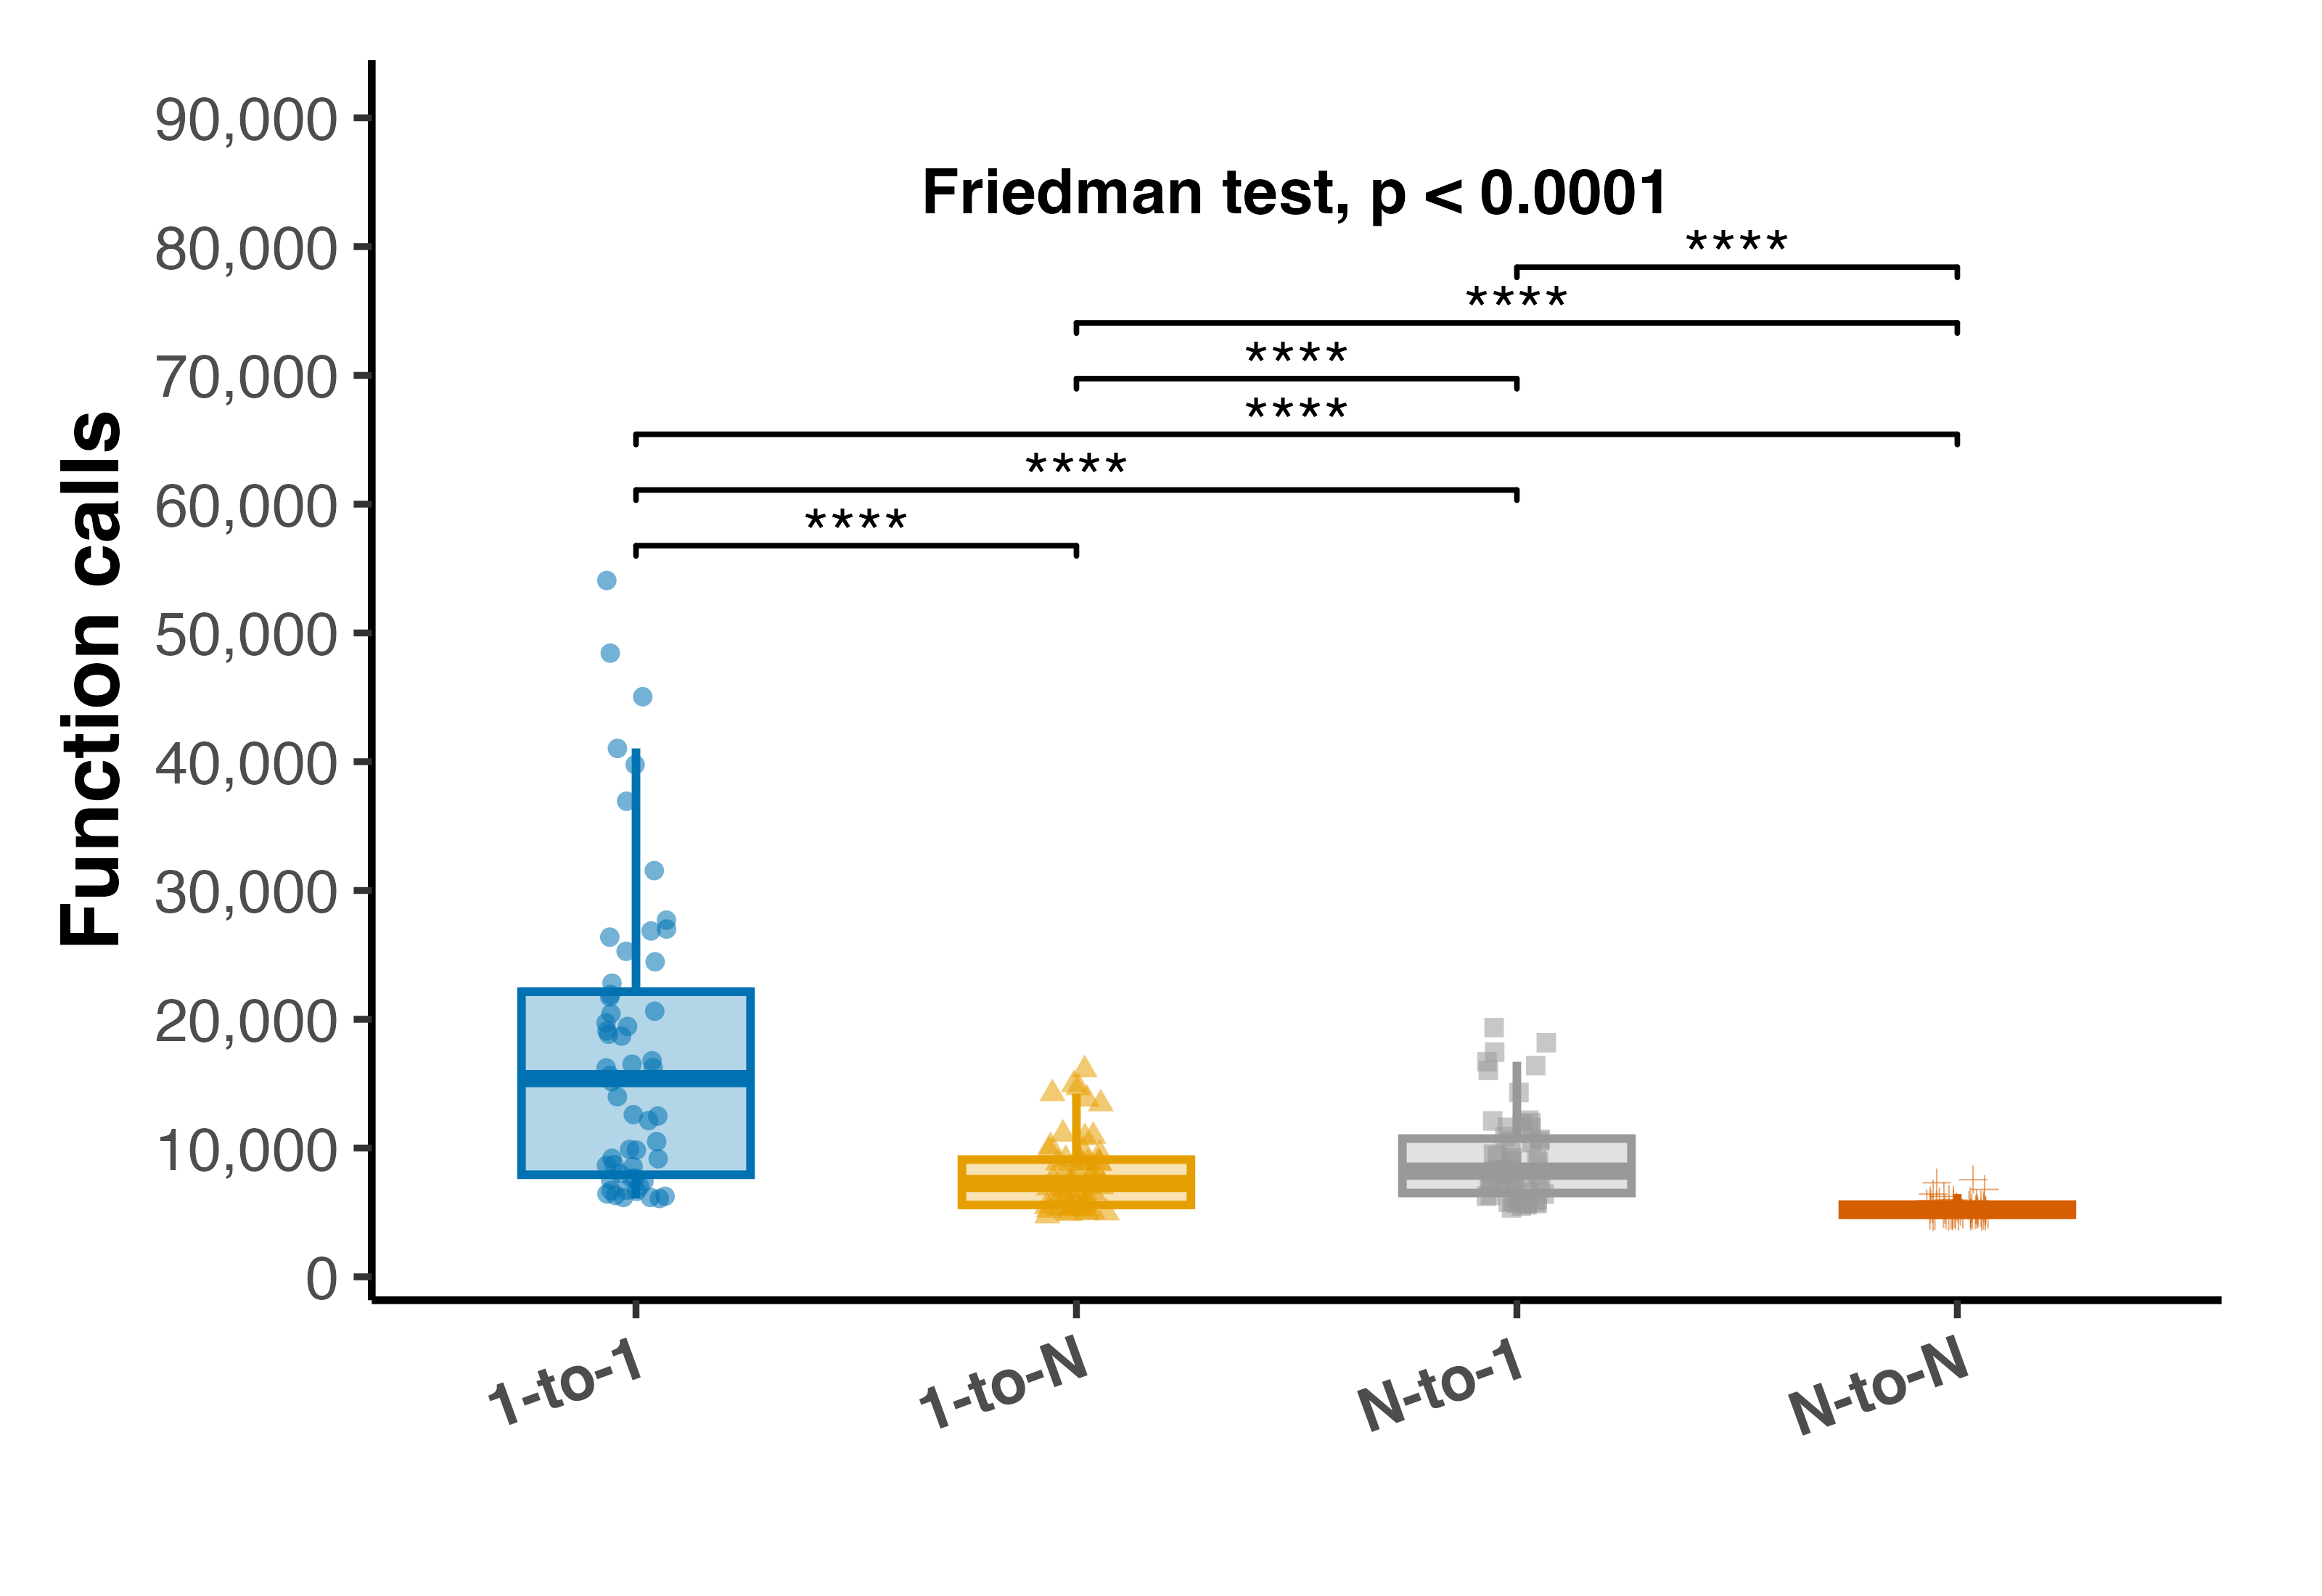
\includegraphics[scale=0.5]{propagation_subpopulation10}

\caption{Impact of Communication Strategies with 10 Subpopulations.\label{fig:Communication-Strategy-with}}
\end{figure}

Figure \ref{fig:Communication-Strategy-with}\textbf{ }illustrates
the effect of different communication strategies among subpopulations
when 10 subpopulations are employed. The four communication schemes
considered are 1to1, 1toN, Nto1 and NtoN each representing a different
mechanism for propagating information throughout the population. The
comparison is based on the total number of objective function evaluations
required to reach convergence where lower values indicate higher optimization
efficiency. As shown in the figure the NtoN communication strategy
achieves the lowest median number of function evaluations and exhibits
the smallest variability among all configurations. The distribution
of results is concentrated within a narrow range of lower values indicating
both faster and more stable convergence. In contrast, the 1to1 strategy
requires substantially more function evaluations and displays the
largest dispersion suggesting slower convergence and greater sensitivity
to problem characteristics. The 1toN and Nto1 strategies provide intermediate
performance improving upon the basic 1to1 communication model but
remaining less effective than the fully connected NtoN scheme. To
evaluate the statistical significance of the observed differences
a Friedman test was performed across all communication strategies.
The obtained result (p \textless{} 0.0001) indicates that at least
one communication scheme differs significantly from the others. Subsequently,
pairwise comparisons were conducted using the Wilcoxon signed-rank
test following the conventional significance notation (ns: p \textgreater{}
0.05, {*}: p \textless{} 0.05, {*}{*}: p \textless{} 0.01, {*}{*}{*}:
p \textless{} 0.001, {*}{*}{*}{*}: p \textless{} 0.0001). The presence
of multiple pairwise comparisons marked with {*}{*}{*}{*} demonstrates
that the differences among the examined communication strategies are
highly statistically significant. In particular, the NtoN strategy
consistently achieves the lowest number of function evaluations significantly
outperforming the 1to1, 1toN and Nto1 configurations. These results
highlight the benefits of allowing all subpopulations to exchange
information simultaneously. Such a communication mechanism accelerates
the dissemination of high-quality solutions throughout the population
enhances cooperation among subpopulations and reduces redundant exploration
of the search space. Overall, the results demonstrate that increasing
the degree of information sharing among subpopulations leads to substantial
improvements in optimization efficiency. Among the examined communication
schemes the NtoN strategy emerges as the most effective approach achieving
the lowest computational cost the lowest variability and the most
consistent convergence behavior across the benchmark problems. 

\subsection{The proposed method in comparison with other methods}

Table \ref{tab:The proposed method in comparison with others}\textbf{
}presents a comparative evaluation of the proposed optimization algorithm
against several well-established metaheuristic methods namely GA \citep{Genetic,Genetic-1},
DE \citep{DE,DE1}, GWO \citep{GWO,GWO1}, ParallelDE \citep{PARALLELDE,PARALLELDE-1},
SAOP \citep{SAOP}, BGWO \citep{BGWO1,BGWO2} and WOA \citep{woa,Woa1}
in terms of the average number of objective function evaluations required
to reach convergence. The experiments were conducted on a diverse
set of benchmark functions with dimensions 25, 50, 100 and 150, where
lower values indicate higher optimization efficiency. The results
demonstrate that the proposed method achieves highly competitive performance
across the benchmark suite and consistently maintains a low computational
cost regardless of problem dimension. In many high-dimensional and
difficult optimization problems the proposed approach requires substantially
fewer function evaluations than most of the competing algorithms.
For example, in Zakharov\_150 the proposed method converges using
only 4927 function evaluations, compared to 38858, 14744, 3251, 5613,
4341, 3333 and 11943 evaluations required by GA, DE, GWO, ParallelDE,
SAOP, BGWO and WOA respectively. Similarly, in Sharp Ridge\_150 the
proposed algorithm requires 5640 evaluations whereas the corresponding
values for GA, DE, GWO, ParallelDE, SAOP, BGWO and WOA are 12266,
12231, 25399, 5614, 4055, 24923 and 8022, respectively. The proposed
method also exhibits remarkable stability across different classes
of optimization problems. Unlike several competing algorithms whose
computational cost increases significantly with problem dimensionality
the proposed approach maintains relatively consistent performance
on multimodal ill-conditioned and non-separable functions. This behavior
suggests that the cooperative search mechanism and the information-sharing
strategy among subpopulations effectively balance exploration and
exploitation allowing the algorithm to avoid premature convergence
while preserving rapid progress toward promising regions of the search
space. The overall computational effort further highlights the effectiveness
of the proposed framework. The total number of function evaluations
accumulated over all benchmark problems is 277,297 for the proposed
method compared with 777,899 for GA, 762,504 for DE, 772,866 for GWO,
314,144 for ParallelDE, 263,370 for SAOP, 724,617 for BGWO and 371,962
for WOA. Consequently, the proposed algorithm achieves a reduction
in computational cost of approximately 64\% compared to GA 64\% compared
to DE 64\% compared to GWO 12\% compared to ParallelDE 62\% compared
to BGWO and 25\% compared to WOA. Although SAOP attains a slightly
lower overall number of function evaluations, the proposed method
remains highly competitive while offering a more consistent performance
profile across the complete benchmark set. Overall, the results indicate
that the integration of cooperative subpopulations efficient information
dissemination and parallel search mechanisms significantly enhances
the optimization capability of the proposed algorithm. The method
demonstrates strong scalability with increasing dimensionality and
achieves a favorable balance between convergence speed and search
robustness, making it a promising approach for solving complex large-scale
optimization problems.

{\scriptsize{}
\begin{table}[H]
\caption{Comparison of the proposed method against competing metaheuristic
algorithms in terms of average objective function evaluations.\label{tab:The proposed method in comparison with others}}

{\tiny{}%
\begin{tabular}{|c|c|c|c|c|c|c|c|c|}
\hline 
{\tiny\textbf{FUNCTION}} & {\tiny\textbf{GA}} & {\tiny\textbf{DE}} & {\tiny\textbf{GWO}} & {\tiny\textbf{PARALLELDE}} & {\tiny\textbf{SAOP}} & {\tiny\textbf{BGWO}} & {\tiny\textbf{WOA}} & {\tiny\textbf{PROPOSED}}\tabularnewline
\hline 
\hline 
\begin{cellvarwidth}[t]
\centering
{\tiny ATTRACTIVE}{\tiny\par}

{\tiny SECTOR\_25}
\end{cellvarwidth} & 2281 & 2234 & 3772 & 5594 & 1715 & 3239 & 1944 & {\small 4701}\tabularnewline
\hline 
\begin{cellvarwidth}[t]
\centering
{\tiny ATTRACTIVE}{\tiny\par}

{\tiny SECTOR\_50}
\end{cellvarwidth} & 2297 & 2298 & 12556 & 5611 & 2106 & 17575 & 4646 & {\small 4873}\tabularnewline
\hline 
\begin{cellvarwidth}[t]
\centering
{\tiny ATTRACTIVE}{\tiny\par}

{\tiny SECTOR\_100}
\end{cellvarwidth} & 2344 & 2273 & 29011 & 5623 & 2691 & 28735 & 6739 & {\small 4964}\tabularnewline
\hline 
\begin{cellvarwidth}[t]
\centering
{\tiny ATTRACTIVE}{\tiny\par}

{\tiny SECTOR\_150}
\end{cellvarwidth} & 2345 & 2255 & 25348 & 5614 & 2618 & 24872 & 6070 & {\small 4927}\tabularnewline
\hline 
{\tiny BUCHE RASTRIGIN\_25} & 11233(0.93) & 11417(0.93) & 4214 & 5592 & 2183(0.93) & 1989(0.93) & 3009(0.97) & {\small 4866}\tabularnewline
\hline 
{\tiny BUCHE RASTRIGIN\_50} & 17589(0.57) & 21873(0.57) & 13509(0.90) & 5610 & 4657(0.57) & 4033(0.57) & 14163(0.70) & {\small 5874}\tabularnewline
\hline 
{\tiny BUCHE RASTRIGIN\_100} & 32881(0.30) & 39401(0.30) & 23867(0.80) & 5622 & 7806(0.30) & 7564(0.30) & 7293(0.97) & {\small 6429}\tabularnewline
\hline 
{\tiny BUCHE RASTRIGIN\_150} & 36444(0.40) & 48017(0.40) & 22139(0.87) & 5611 & 7731(0.40) & 6472(0.40) & 5699 & {\small 4715}\tabularnewline
\hline 
{\tiny DISCUS\_25} & 2715 & 2612 & 4979 & 5596 & 1747 & 4266 & 2505 & {\small 4905}\tabularnewline
\hline 
{\tiny DISCUS\_50} & 2714 & 2701 & 19111 & 5614 & 2472 & 18438 & 8241 & {\small 4994}\tabularnewline
\hline 
{\tiny DISCUS\_100} & 2752 & 2693 & 29094 & 5624 & 2722 & 28740 & 12795 & {\small 5083}\tabularnewline
\hline 
{\tiny DISCUS\_150} & 2750 & 2671 & 25351 & 5614 & 2483 & 24876 & 11185 & {\small 4818}\tabularnewline
\hline 
{\tiny DIFFERENTPOWERS\_25} & 13758 & 14154 & 3580 & 5595 & 2456 & 2728 & 1864 & {\small 5575}\tabularnewline
\hline 
{\tiny DIFFERENTPOWERS\_50} & 19777 & 22093 & 10497 & 5612 & 8075 & 12334 & 4211 & {\small 6784}\tabularnewline
\hline 
{\tiny DIFFERENTPOWERS\_100} & 28988 & 29193 & 25884 & 5624 & 13699 & 27204 & 6439 & {\small 5957}\tabularnewline
\hline 
{\tiny DIFFERENTPOWERS\_150} & 34372 & 34490 & 25642 & 5613 & 15676 & 25413 & 5930 & {\small 5911}\tabularnewline
\hline 
{\tiny ELLIPSOIDAL\_25} & 5930 & 5778 & 3598 & 5593 & 1847 & 2778 & 1843 & {\small 4773}\tabularnewline
\hline 
{\tiny ELLIPSOIDAL\_50} & 10583 & 11023 & 10624 & 5611 & 2979 & 13691 & 4127 & {\small 5595}\tabularnewline
\hline 
{\tiny ELLIPSOIDAL\_100} & 20604 & 20345 & 25068 & 5623 & 5137 & 28976 & 6014 & {\small 7303}\tabularnewline
\hline 
{\tiny ELLIPSOIDAL\_150} & 28556 & 27643 & 25642 & 5612 & 5893 & 25171 & 5653 & {\small 7541}\tabularnewline
\hline 
{\tiny GALLAGHER21\_25} & 3118(0.93) & 2867(0.93) & 3214(0.93) & 5595 & 2206(0.93) & 2115(0.93) & 3978(0.93) & {\small 4773}\tabularnewline
\hline 
{\tiny GALLAGHER21\_50} & 3272(0.57) & 3566(0.57) & 6234(0.57) & 5612 & 8557(0.57) & 6590(0.57) & 14831(0.57) & {\small 5277}\tabularnewline
\hline 
{\tiny GALLAGHER21\_100} & 1693(0.30) & 1621(0.30) & 2901(0.30) & 5622 & 1691(0.30) & 8781(0.30) & 1502(0.30) & {\small 5305}\tabularnewline
\hline 
{\tiny GALLAGHER21\_150} & 1682(0.40) & 1617(0.40) & 2898(0.40) & 5613 & 1671(0.40) & 1703(0.40) & 1500(0.40) & {\small 5298}\tabularnewline
\hline 
{\tiny GALLAGHER101\_25} & 3083(0.93) & 3030(0.93) & 3106(0.93) & 5593 & 2068 & 1913(0.93) & 3531(0.93) & {\small 4767}\tabularnewline
\hline 
{\tiny GALLAGHER101\_50} & 6150(0.57) & 4617(0.57) & 5873(0.57) & 5602 & 6932 & 7429(0.57) & 13266(0.57) & {\small 5238}\tabularnewline
\hline 
{\tiny GALLAGHER101\_100} & 6656(0.30) & 4340(0.30) & 8356(0.30) & 5606 & 18872 & 12116(0.30) & 18537(0.30) & {\small 5452}\tabularnewline
\hline 
{\tiny GALLAGHER101\_150} & 6122(0.40) & 3236(0.40) & 7496(0.40) & 5601 & 19066 & 14717(0.40) & 15220(0.40) & {\small 5217}\tabularnewline
\hline 
{\tiny GRIEWANK \_25} & 9514 & 9655 & 3695(0.97) & 5594 & 2237 & 2878(0.97) & 1893 & {\small 4833}\tabularnewline
\hline 
{\tiny GRIEWANK \_50} & 5511 & 5147 & 10342(0.97) & 5610 & 3132 & 12370(0.83) & 4184 & {\small 5557}\tabularnewline
\hline 
{\tiny GRIEWANK \_100} & 5078 & 4141 & 22295 & 5623 & 4053 & 27343(0.87) & 6532(0.97) & {\small 6246}\tabularnewline
\hline 
{\tiny GRIEWANK \_150} & 5284 & 4131 & 25374 & 5612 & 3934 & 24895(0.93) & 6098(0.97) & {\small 5820}\tabularnewline
\hline 
{\tiny GRIEWANK\_ROSENBROCK\_25} & 16098 & 17837 & 3429 & 5595 & 2259 & 2435 & 1740 & {\small 4754}\tabularnewline
\hline 
{\tiny GRIEWANK\_ROSENBROCK\_50} & 22598 & 27316 & 8659 & 5612 & 4413 & 9859 & 3361 & {\small 5299}\tabularnewline
\hline 
{\tiny GRIEWANK\_ROSENBROCK\_100} & 30869 & 35225 & 19410 & 5624 & 5856 & 21301 & 4784 & {\small 5536}\tabularnewline
\hline 
{\tiny GRIEWANK\_ROSENBROCK\_150} & 37686 & 40126 & 22950 & 5613 & 6664 & 23047 & 4450 & {\small 5287}\tabularnewline
\hline 
{\tiny ROSENBROCK\_25} & 15148 & 15199 & 3760 & 5595 & 2217 & 3320 & 1925 & {\small 4728}\tabularnewline
\hline 
{\tiny ROSENBROCK\_50} & 23663 & 25189 & 12789 & 5612 & 4238 & 18057 & 4611 & {\small 5083}\tabularnewline
\hline 
{\tiny ROSENBROCK\_100} & 40370 & 39254 & 29103 & 5623 & 7197 & 28756 & 6786 & {\small 5145}\tabularnewline
\hline 
{\tiny ROSENBROCK\_150} & 53927 & 51902 & 25367 & 5613 & 8677 & 24893 & 6076 & {\small 4958}\tabularnewline
\hline 
{\tiny RARSTIGIN\_25} & 9348(0.93) & 9799(0.93) & 2959(0.93) & 5594 & 2067(0.93) & 2007(0.93) & 3007(0.97) & {\small 4869}\tabularnewline
\hline 
{\tiny RARSTIGIN\_50} & 11414(0.57) & 13738(0.57) & 13386(0.87) & 5610 & 3871(0.57) & 4022(0.57) & 15194(0.67) & {\small 5675}\tabularnewline
\hline 
{\tiny RARSTIGIN\_100} & 12898(0.30) & 17722(0.30) & 22715(0.77) & 5622 & 4840(0.30) & 7611(0.30) & 10638(0.87) & {\small 5999}\tabularnewline
\hline 
{\tiny RARSTIGIN\_150} & 14392(0.40) & 19506(0.40) & 18708(0.73) & 5612 & 4693(0.40) & 6693(0.40) & 6827(0.97) & {\small 5686}\tabularnewline
\hline 
{\tiny STEP ELLIPSOIDAL\_25} & 1718(0.93) & 1664(0.93) & 3078 & 5593 & 1806(0.93) & 1831 & 1590 & {\small 4669}\tabularnewline
\hline 
{\tiny STEP ELLIPSOIDAL\_50} & 2201(0.57) & 1661(0.57) & 5163 & 5610 & 2369(0.57) & 3615(0.90) & 2273(0.93) & {\small 4699}\tabularnewline
\hline 
{\tiny STEP ELLIPSOIDAL\_100} & 2028(0.30) & 1629(0.30) & 10101(0.97) & 5622 & 2355(0.30) & 6624(0.57) & 2708(0.97) & {\small 4701}\tabularnewline
\hline 
{\tiny STEP ELLIPSOIDAL\_150} & 1752(0.40) & 1617(0.40) & 12778(0.97) & 5612 & 1977(0.40) & 6730(0.44) & 2527(0.97) & {\small 4695}\tabularnewline
\hline 
{\tiny SHARP RIDGE\_25} & 11324 & 11800 & 4098 & 5596 & 2124 & 4087 & 2110 & {\small 4795}\tabularnewline
\hline 
{\tiny SHARP RIDGE\_50} & 11454 & 12866 & 16581 & 5612 & 3106 & 18454 & 5907 & {\small 5338}\tabularnewline
\hline 
{\tiny SHARP RIDGE\_100} & 12105 & 12682 & 29123 & 5624 & 3995 & 28790 & 8936 & {\small 5644}\tabularnewline
\hline 
{\tiny SHARP RIDGE\_150} & 12266 & 12231 & 25399 & 5614 & 4055 & 24923 & 8022 & {\small 5640}\tabularnewline
\hline 
{\tiny ZAKHAROV\_25} & 5760 & 4939 & 8426 & 5598 & 2177 & 9075 & 10581 & {\small 4827}\tabularnewline
\hline 
{\tiny ZAKHAROV\_50} & 15253 & 8154 & 23034 & 5611 & 3083 & 27447 & 25061 & {\small 5179}\tabularnewline
\hline 
{\tiny ZAKHAROV\_100} & 36693 & 12572 & 3329 & 5623 & 3878 & 5763 & 9463 & {\small 4803}\tabularnewline
\hline 
{\tiny ZAKHAROV\_150} & 38858 & 14744 & 3251 & 5613 & 4341 & 3333 & 11943 & {\small 4919}\tabularnewline
\hline 
 & 777899(0.84) & 762504(0.84) & 772866(0.91) & 314144 & 263370(0.84) & 724617(0.85) & 371962(0.92) & {\small 297299}\tabularnewline
\hline 
\end{tabular}}{\tiny\par}
\end{table}
}{\scriptsize\par}

\begin{figure}

\includegraphics[scale=0.6]{methods}\caption{The proposed method in comparison with others.\label{fig:The-proposed-method}}
\end{figure}

Figure\textbf{ }\ref{fig:The-proposed-method} presents a comparative
analysis of the examined optimization algorithms in terms of the number
of objective function evaluations required to achieve convergence.
The comparison includes GENETIC (GA), DE, GWO, PARALLELDE, SAOP, BGWO,
WOA and the PROPOSED method. Since the number of function evaluations
represents a direct measure of computational effort, lower values
indicate higher optimization efficiency.

As illustrated in the figure the PROPOSED algorithm exhibits one of
the lowest median numbers of function evaluations while also maintaining
the smallest variability among the examined methods. The narrow distribution
of results indicates a high degree of robustness and consistent convergence
behavior across the benchmark problems. In contrast, the GENETIC,
WOA, BGWO and PARALLELDE algorithms display substantially larger dispersion
and generally higher evaluation counts suggesting increased computational
requirements and less stable convergence performance. The DE GWO and
SAOP algorithms also achieve relatively low numbers of function evaluations
however, they exhibit either greater variability or less consistent
behavior compared with the proposed method. To assess whether the
observed differences are statistically significant a Kruskal--Wallis
non-parametric test was performed. The obtained result (p \textless{}
0.0001) indicates that statistically significant differences exist
among the compared algorithms. Consequently, the null hypothesis that
all algorithms exhibit identical performance distributions can be
rejected with a high level of confidence. The reduced spread of the
proposed method combined with its consistently low number of function
evaluations suggests that the algorithm is able to efficiently balance
exploration and exploitation throughout the optimization process.
This behavior can be attributed to the cooperative subpopulation structure
the information dissemination mechanism and the parallel search strategy
incorporated into the proposed framework which collectively facilitate
the rapid discovery and propagation of high-quality solutions. Overall,
the results demonstrate that the proposed approach combines low computational
cost with highly stable convergence behavior. The combination of efficiency
robustness and consistency across a diverse set of benchmark functions
highlights the effectiveness of the proposed method for solving complex
optimization problems particularly in high-dimensional search spaces.

\subsection{Practical problems}

To further examine the practical efficiency and scalability of the
proposed optimization algorithm two real-world optimization problems
were investigated: the GasCycle \citep{GasCycle} engineering design
problem and the LennardJones13 \citep{Lennard,Lennard-1} molecular
optimization problem. These problems were selected because they differ
significantly in their mathematical formulation and computational
complexity thereby providing a comprehensive framework for evaluating
the algorithm's performance under diverse and realistic conditions.
Each problem was tested across multiple dimensional configurations
ranging from 25 to 500 variables in order to assess how the algorithm
behaves as the search space becomes more complex. For every configuration
the execution time in seconds was recorded as the main performance
indicator. This experimental setup enables a direct comparison of
how computational efficiency changes with increasing dimensionality.
\begin{itemize}
\item \textbf{GasCycle Thermal Cycle}

Vars: $\bm{x}=[T_{1},T_{3},P_{1},P_{3}]^{\top}$. \quad{}$r=P_{3}/P_{1},\ \gamma=1.4.$
\[
\eta(\bm{x})=1-r^{-(\gamma-1)/\gamma}\,\frac{T_{1}}{T_{3}},\qquad\min_{\bm{x}}f(\bm{x})=-\eta(\bm{x}).
\]
Bounds: $300\!\le\!T_{1}\!\le\!1500,\;1200\!\le\!T_{3}\!\le\!2000,\;1\!\le\!P_{1},P_{3}\!\le\!20.$

Penalty: infeasible $\Rightarrow f=10^{20}$.

The GasCycle scenario presents a more computationally demanding optimization
problem, allowing a clearer assessment of algorithmic scalability
under increased complexity.

\begin{figure}[H]

\includegraphics[scale=0.5]{GasCycle}\caption{Comparison of Function Calls Across Dimensions (GasCycle).\label{fig:Comparison-of-Function}}
\end{figure}

\end{itemize}
Figure \ref{fig:Comparison-of-Function} presents the comparison of
the number of objective function evaluations as the problem dimension
increases for the GasCycle benchmark problem. The results indicate
that most algorithms maintain relatively stable performance across
the examined dimensions. The PARALLELDE algorithm consistently requires
the highest number of function evaluations demonstrating a significantly
larger computational cost than the remaining methods. The GENETIC,
DE, GWO, BGWO and WOA algorithms operate at intermediate levels showing
moderate fluctuations as the dimensionality changes. The SAOP method
achieves the lowest number of evaluations overall while the PROPOSED
algorithm exhibits stable and predictable behavior maintaining a nearly
constant number of function calls throughout the entire dimensional
range. Overall the results suggest that the proposed method scales
effectively with increasing dimensionality and preserves a controlled
computational cost making it a reliable approach for high-dimensional
optimization problems.

\begin{figure}[H]

\includegraphics[scale=0.5]{GasCycle1}\caption{Comparison of Execution Time Across Dimensions (GasCycle).\label{fig:Comparison-of-Execution}}
\end{figure}

Figure \ref{fig:Comparison-of-Execution} presents the execution time
of the examined optimization algorithms across different problem dimensions
for the GasCycle benchmark problem. The results indicate that the
execution time increases with the dimensionality of the problem for
all methods reflecting the growing computational complexity associated
with larger search spaces. Among the compared algorithms PARALLELDE
consistently exhibits the highest execution times across all dimensions,
with a noticeably steeper growth rate than the remaining methods.
In contrast GENETIC, GWO, BGWO, SAOP, DE, WOA and the PROPOSED algorithm
demonstrate similar scalability trends, with execution times increasing
in a relatively smooth manner as the dimensionality increases. The
PROPOSED algorithm maintains execution times that are comparable to
those of the other population-based methods throughout the examined
dimensional range. Although its execution time gradually increases
with problem size, the growth remains controlled and follows a pattern
similar to that of DE, BGWO and GWO. Furthermore, the proposed method
avoids the substantial computational overhead observed in PARALLELDE
while preserving stable behavior across all tested dimensions. Overall,
the results suggest that the proposed approach scales effectively
with increasing dimensionality and remains computationally efficient
for solving higher-dimensional instances of the GasCycle optimization
problem.
\begin{itemize}
\item LennardJones13
\item $E(x)$ = $4$ $\sum_{i=1}\mathop{^{N-1}}$$\sum_{j=i+1}\mathop{^{N}}$$\left[\left(\frac{1}{r_{ij}}\right)^{12}-\left(\frac{1}{r_{ij}}\right)^{6}\right]$
\item where $N=13$ denotes the number of atoms and $r_{ij}$ represents
the Euclidean distance between atoms $i$ and $j$ 
\begin{figure}[H]
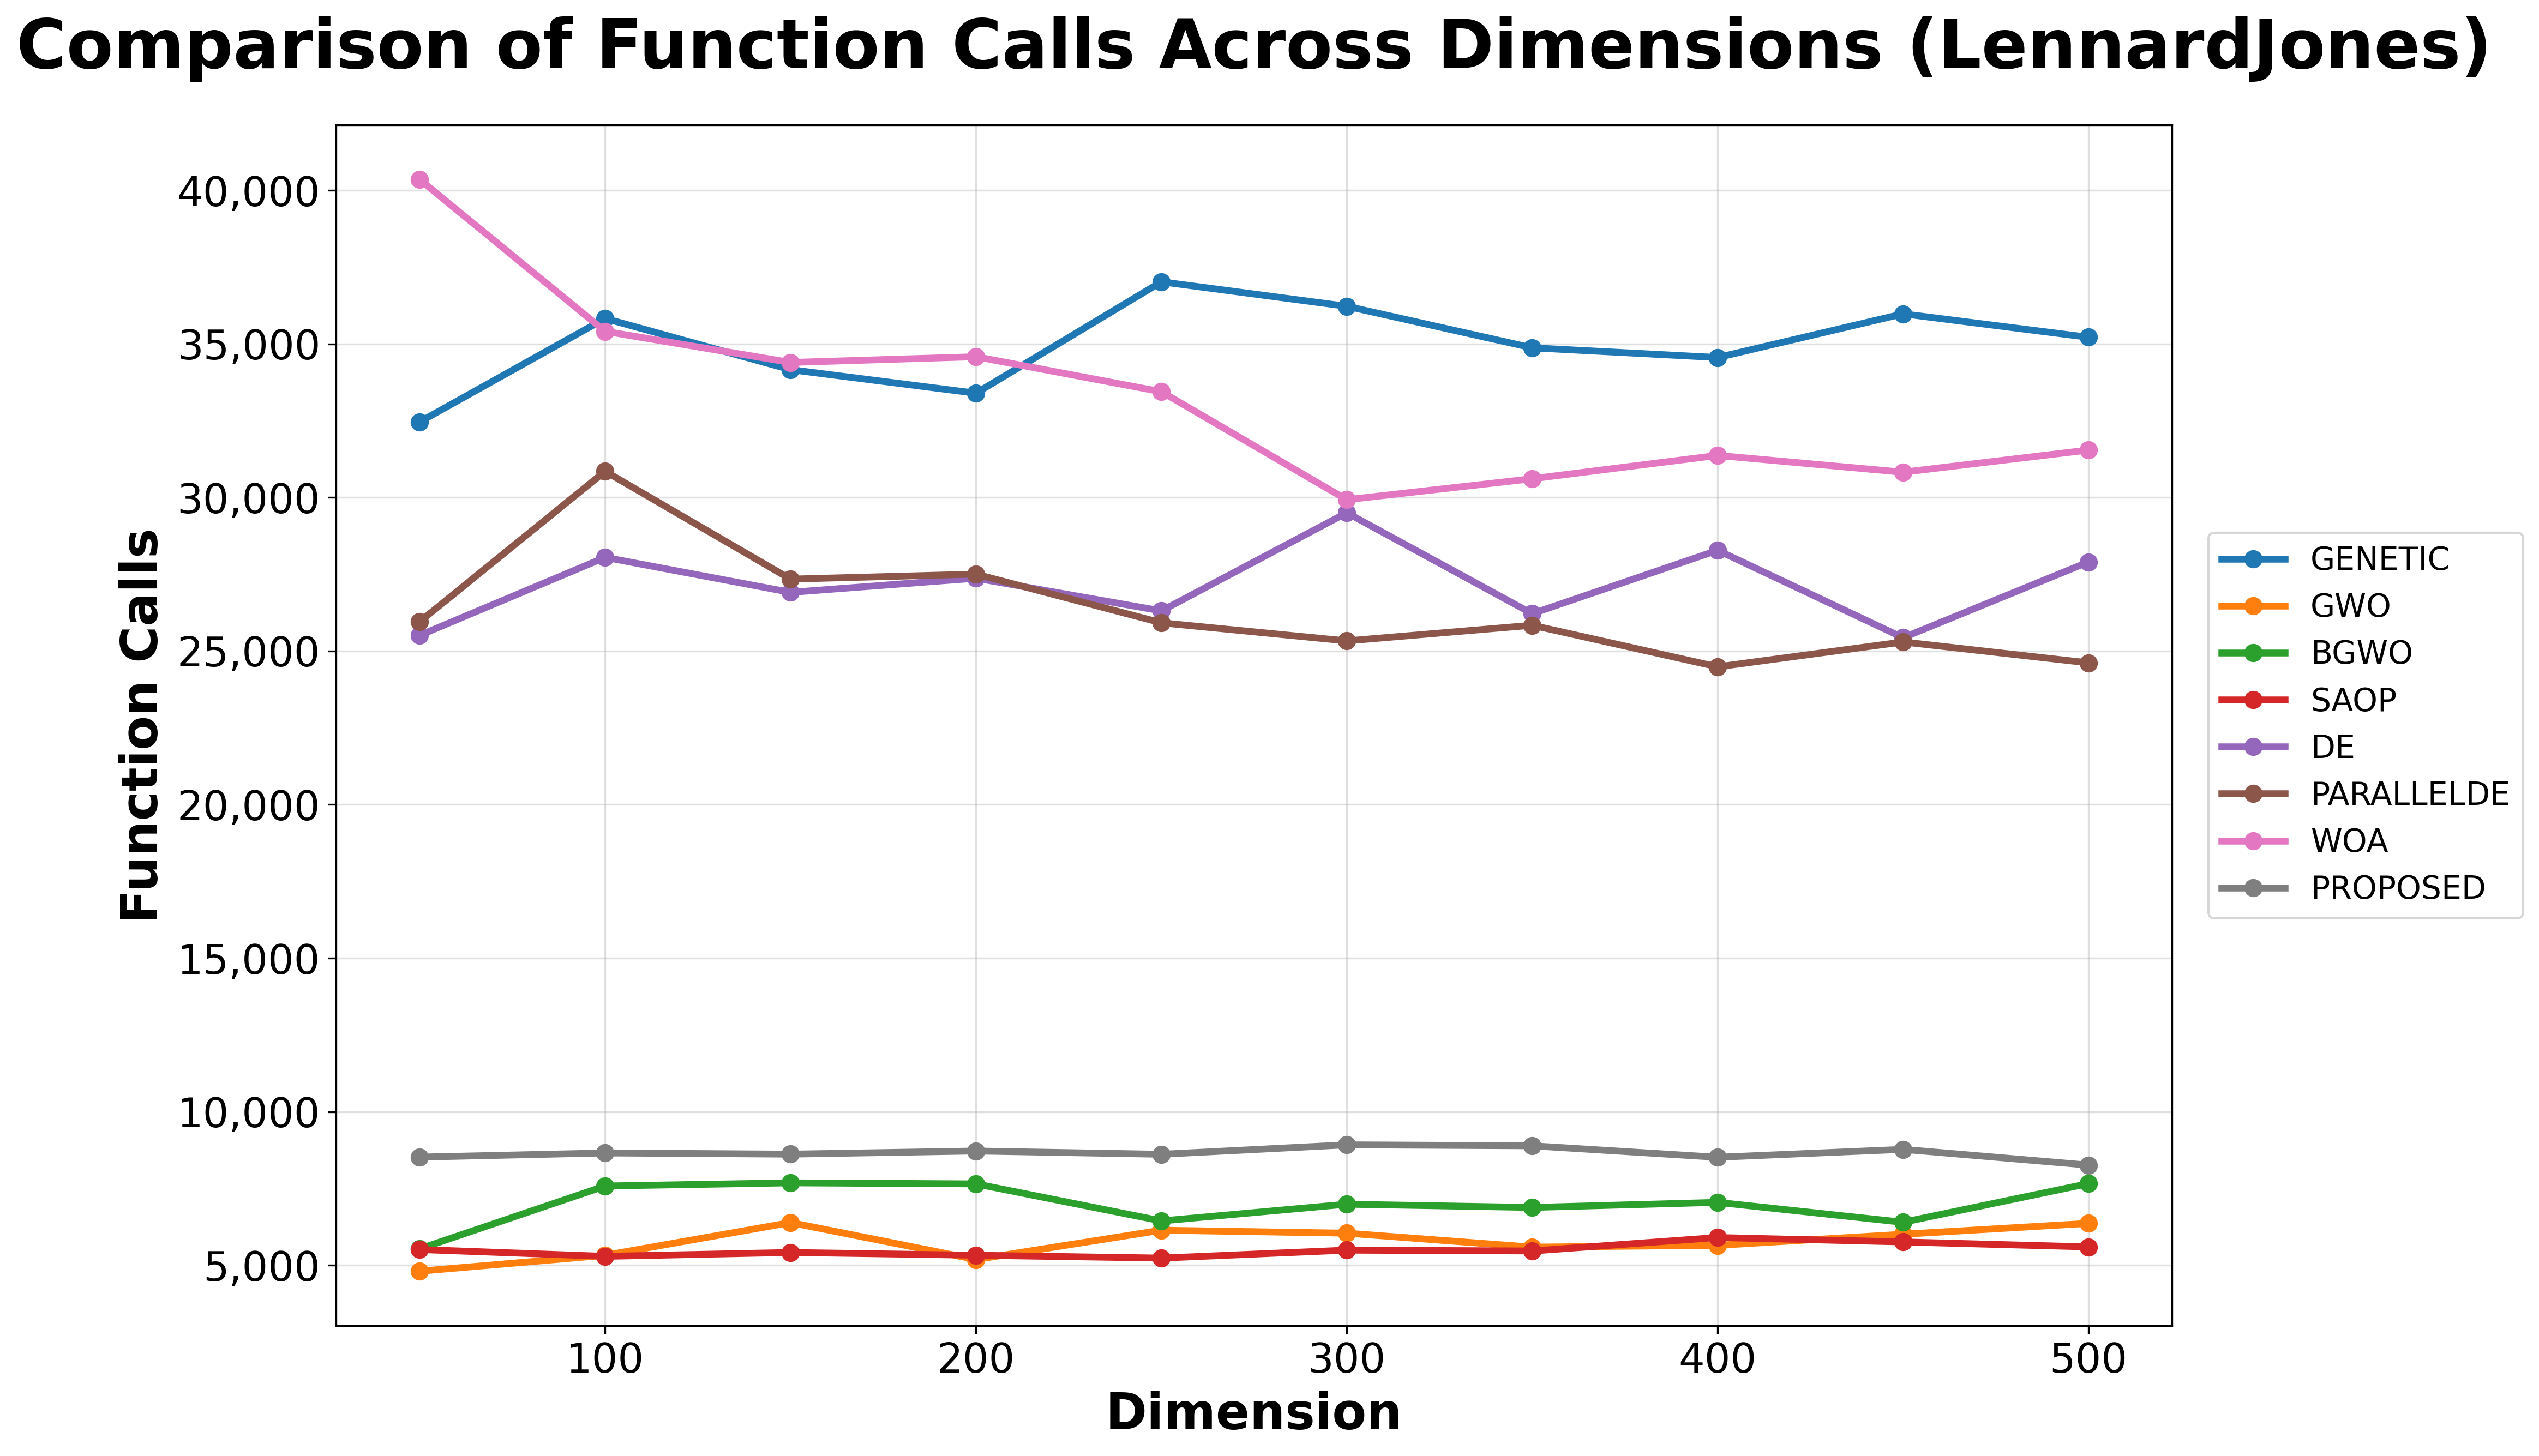
\includegraphics[scale=0.35]{LennardJones_FunctionCalls}\caption{Comparison of Function Calls Across Dimensions (LennardJones13).\label{fig:Comparison-of-Function-1}}
\end{figure}
\end{itemize}
Figure \ref{fig:Comparison-of-Function-1} presents the comparison
of the number of objective function evaluations across different problem
dimensions for the LennardJones13 benchmark problem. The results reveal
clear differences in the computational effort required by the examined
optimization algorithms. The GENETIC, DE, PARALLELDE and WOA algorithms
consistently require a substantially larger number of function evaluations
than the remaining methods indicating a higher computational cost
throughout the examined dimensional range. In contrast GWO, SAOP and
BGWO exhibit lower computational requirements and maintain relatively
stable behavior as the dimensionality increases. The PROPOSED method
demonstrates a stable and predictable performance across all tested
dimensions. Although it does not achieve the lowest number of function
evaluations among the compared algorithms, it consistently requires
fewer evaluations than GENETIC, DE, PARALLELDE and WOA while exhibiting
only minor fluctuations as the problem dimension grows. Furthermore,
the proposed approach maintains a nearly constant computational effort
across the examined dimensional range indicating good scalability
characteristics. Overall, the results suggest that the proposed algorithm
preserves a balanced trade-off between computational cost and robustness
maintaining stable performance as the dimensionality increases. This
behavior highlights the suitability of the proposed method for addressing
higher-dimensional instances of the LennardJones13 optimization problem.

\begin{figure}[H]
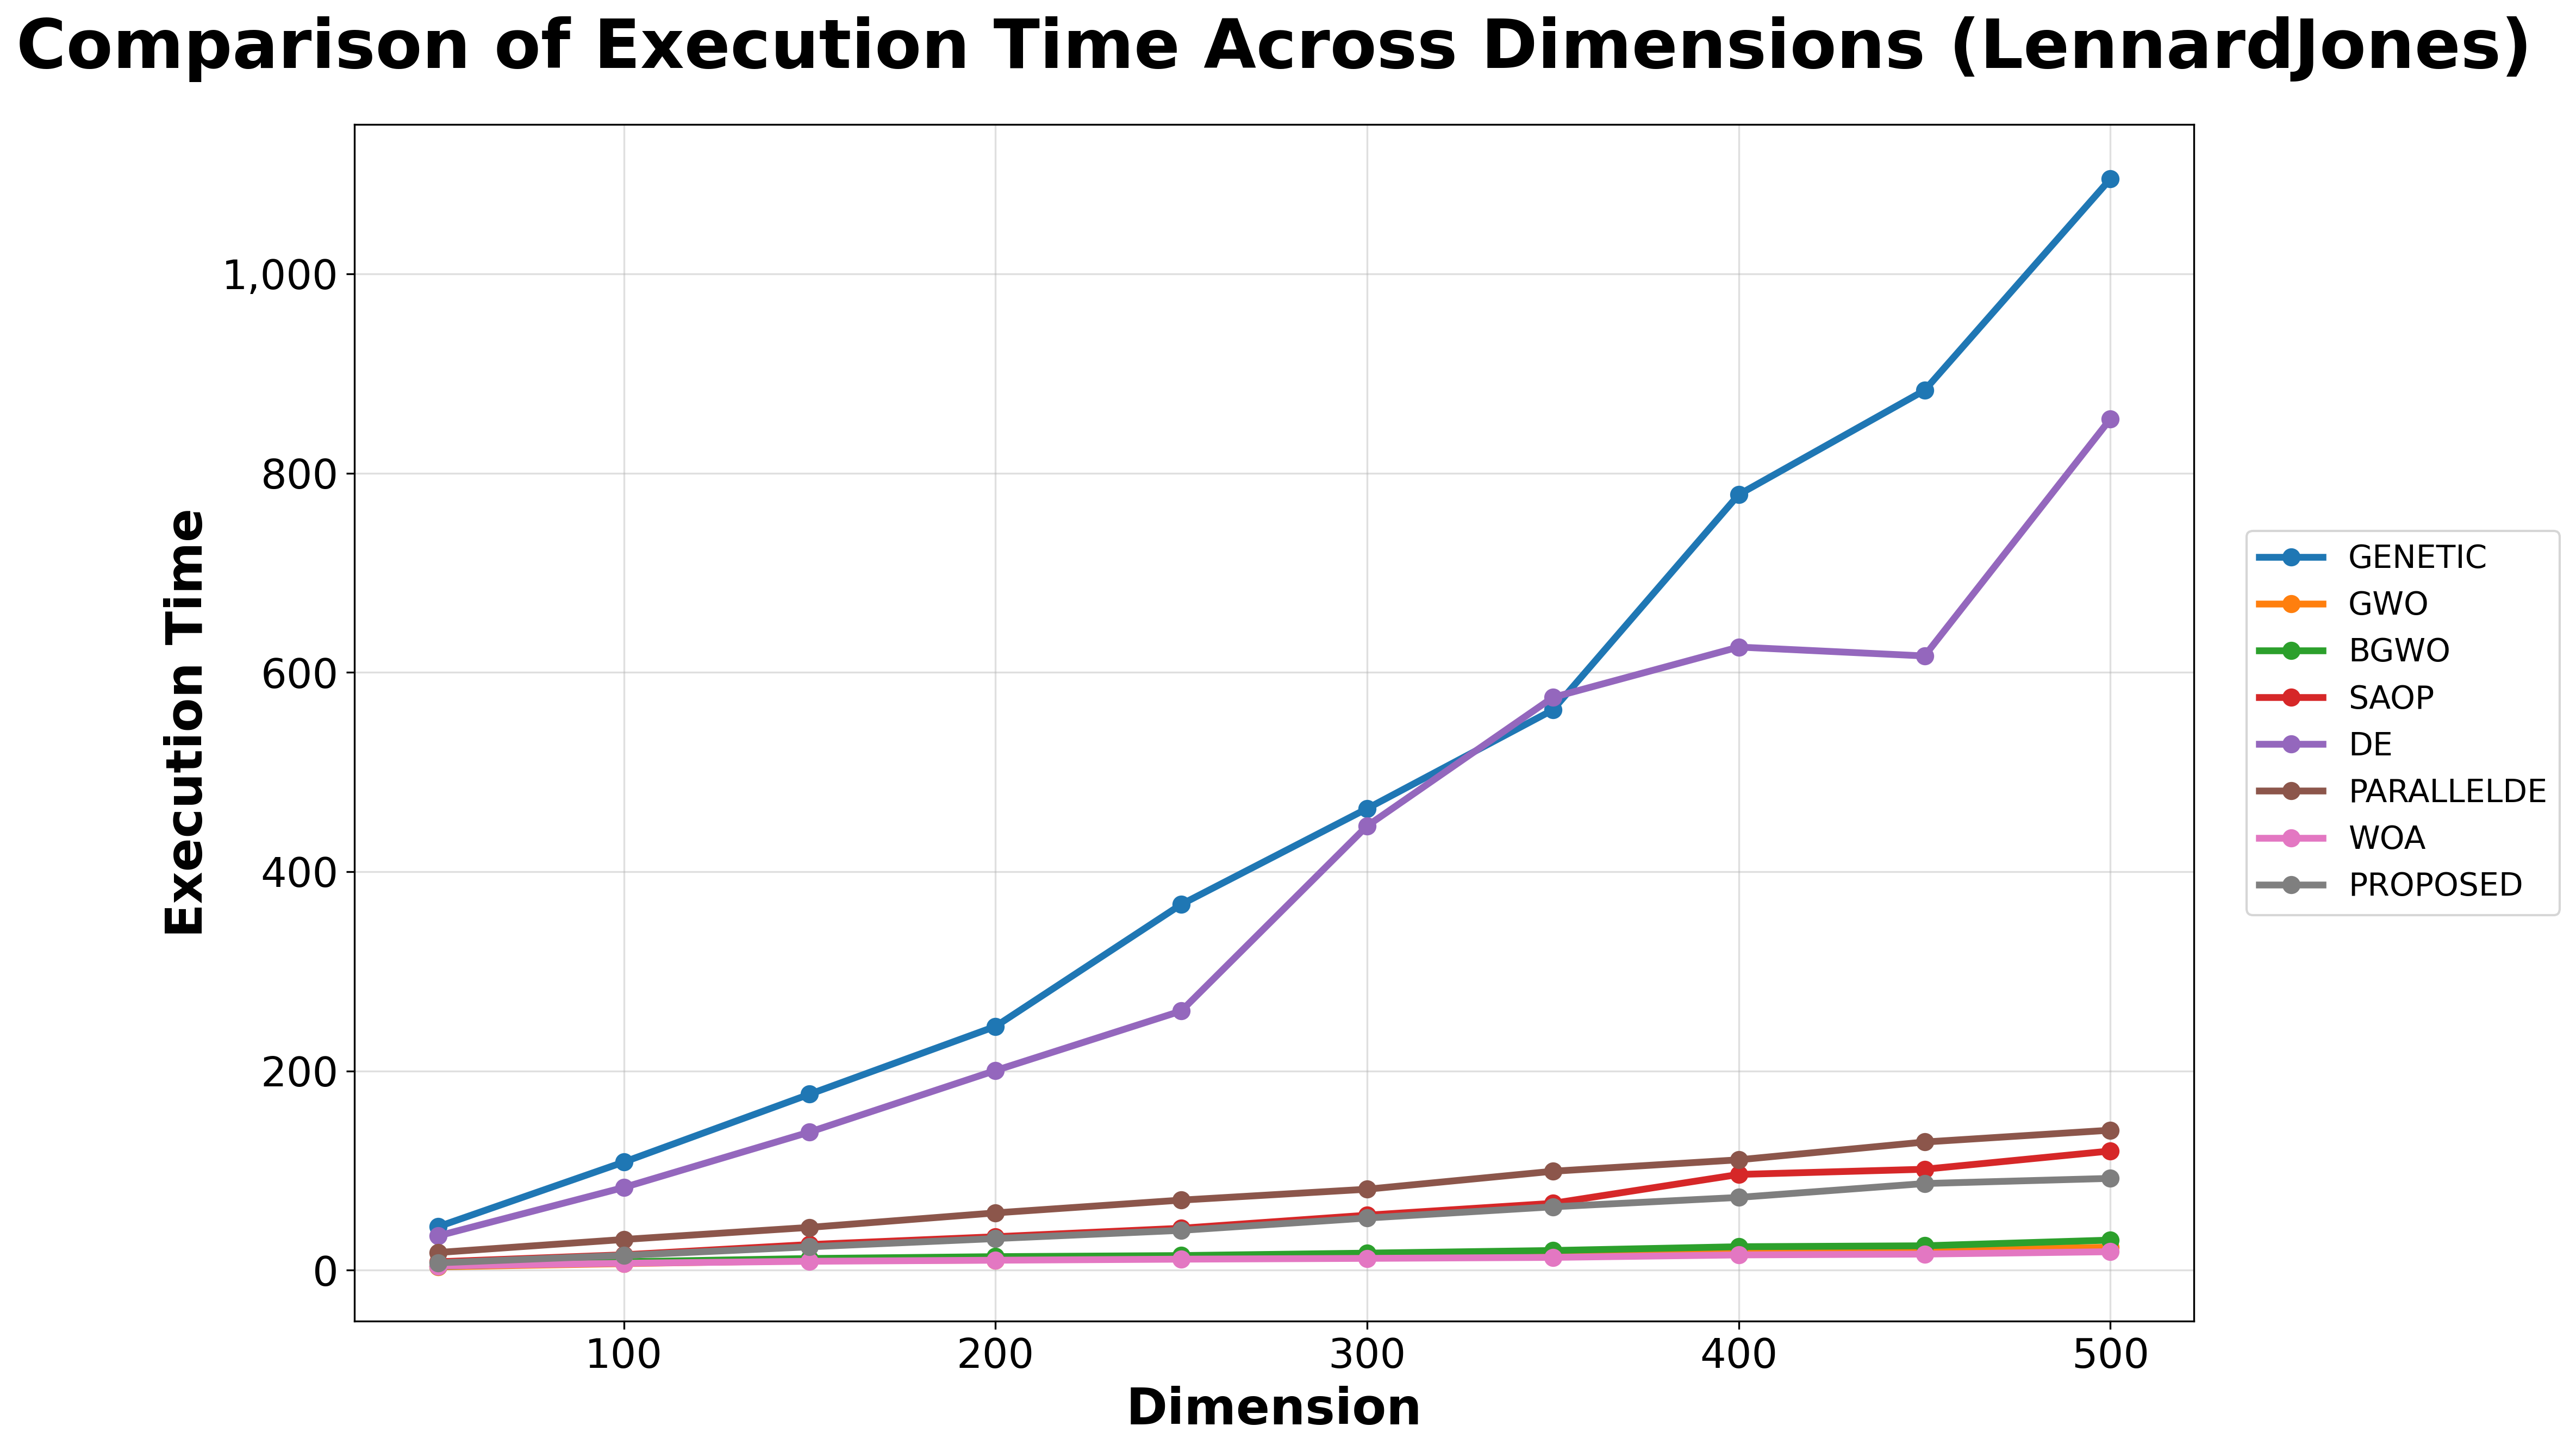
\includegraphics[scale=0.35]{LennardJones_ExecutionTime}\caption{Comparison of Execution Time Across Dimensions (LennardJones13).\label{fig:Comparison-of-Function-2}}
\end{figure}

Figure \ref{fig:Comparison-of-Function-2} presents the execution
time of the examined optimization algorithms as a function of problem
dimensionality for the LennardJones13 benchmark problem. As expected,
the execution time increases with increasing dimension for all methods
due to the higher computational complexity associated with larger
search spaces. The GENETIC and DE algorithms exhibit the steepest
increase in execution time reaching the highest values in the largest
dimensions. PARALLELDE and SAOP also show a noticeable growth in computational
cost although their execution times remain significantly lower than
those of GENETIC and DE. In contrast GWO, BGWO and WOA maintain comparatively
low execution times across the entire dimensional range. The PROPOSED
method demonstrates a stable and predictable increase in execution
time as dimensionality grows. Although its execution time is higher
than that of GWO, BGWO and WOA it remains substantially lower than
the execution times of GENETIC, DE and PARALLELDE, indicating a favorable
trade-off between computational cost and optimization performance.
Overall, the results show that the proposed algorithm scales effectively
with increasing dimensionality while maintaining reasonable execution
times confirming its suitability for solving high-dimensional LennardJones13
optimization problems.

\subsection{Impact of Communication Strategies on Practical Problems}

Figure \ref{fig:Comparison-of-Function-2-1} presents the comparison
of the number of objective function evaluations obtained by the three
communication strategies (STRATEGY1, STRATEGY2 and STRATEGY3) for
the GasCycle benchmark problem across different problem dimensions.
Lower values indicate better optimization efficiency. The results
show that all three strategies exhibit relatively stable behavior
as the dimensionality increases with only moderate fluctuations in
the number of function evaluations. STRATEGY2 generally achieves the
lowest values in most dimensions particularly between 200 and 300
dimensions indicating a lower computational effort. STRATEGY1 follows
a similar trend but with slightly higher variation across dimensions.
In contrast, STRATEGY3 tends to require a larger number of function
evaluations for most problem sizes, although it remains competitive
at higher dimensions. Overall, the differences between the three strategies
are relatively small, suggesting that all communication schemes provide
robust performance on the GasCycle problem. Nevertheless, STRATEGY2
appears to offer the most favorable balance between convergence efficiency
and computational cost achieving the lowest average number of function
evaluations across the examined dimensions.

\begin{figure}[H]
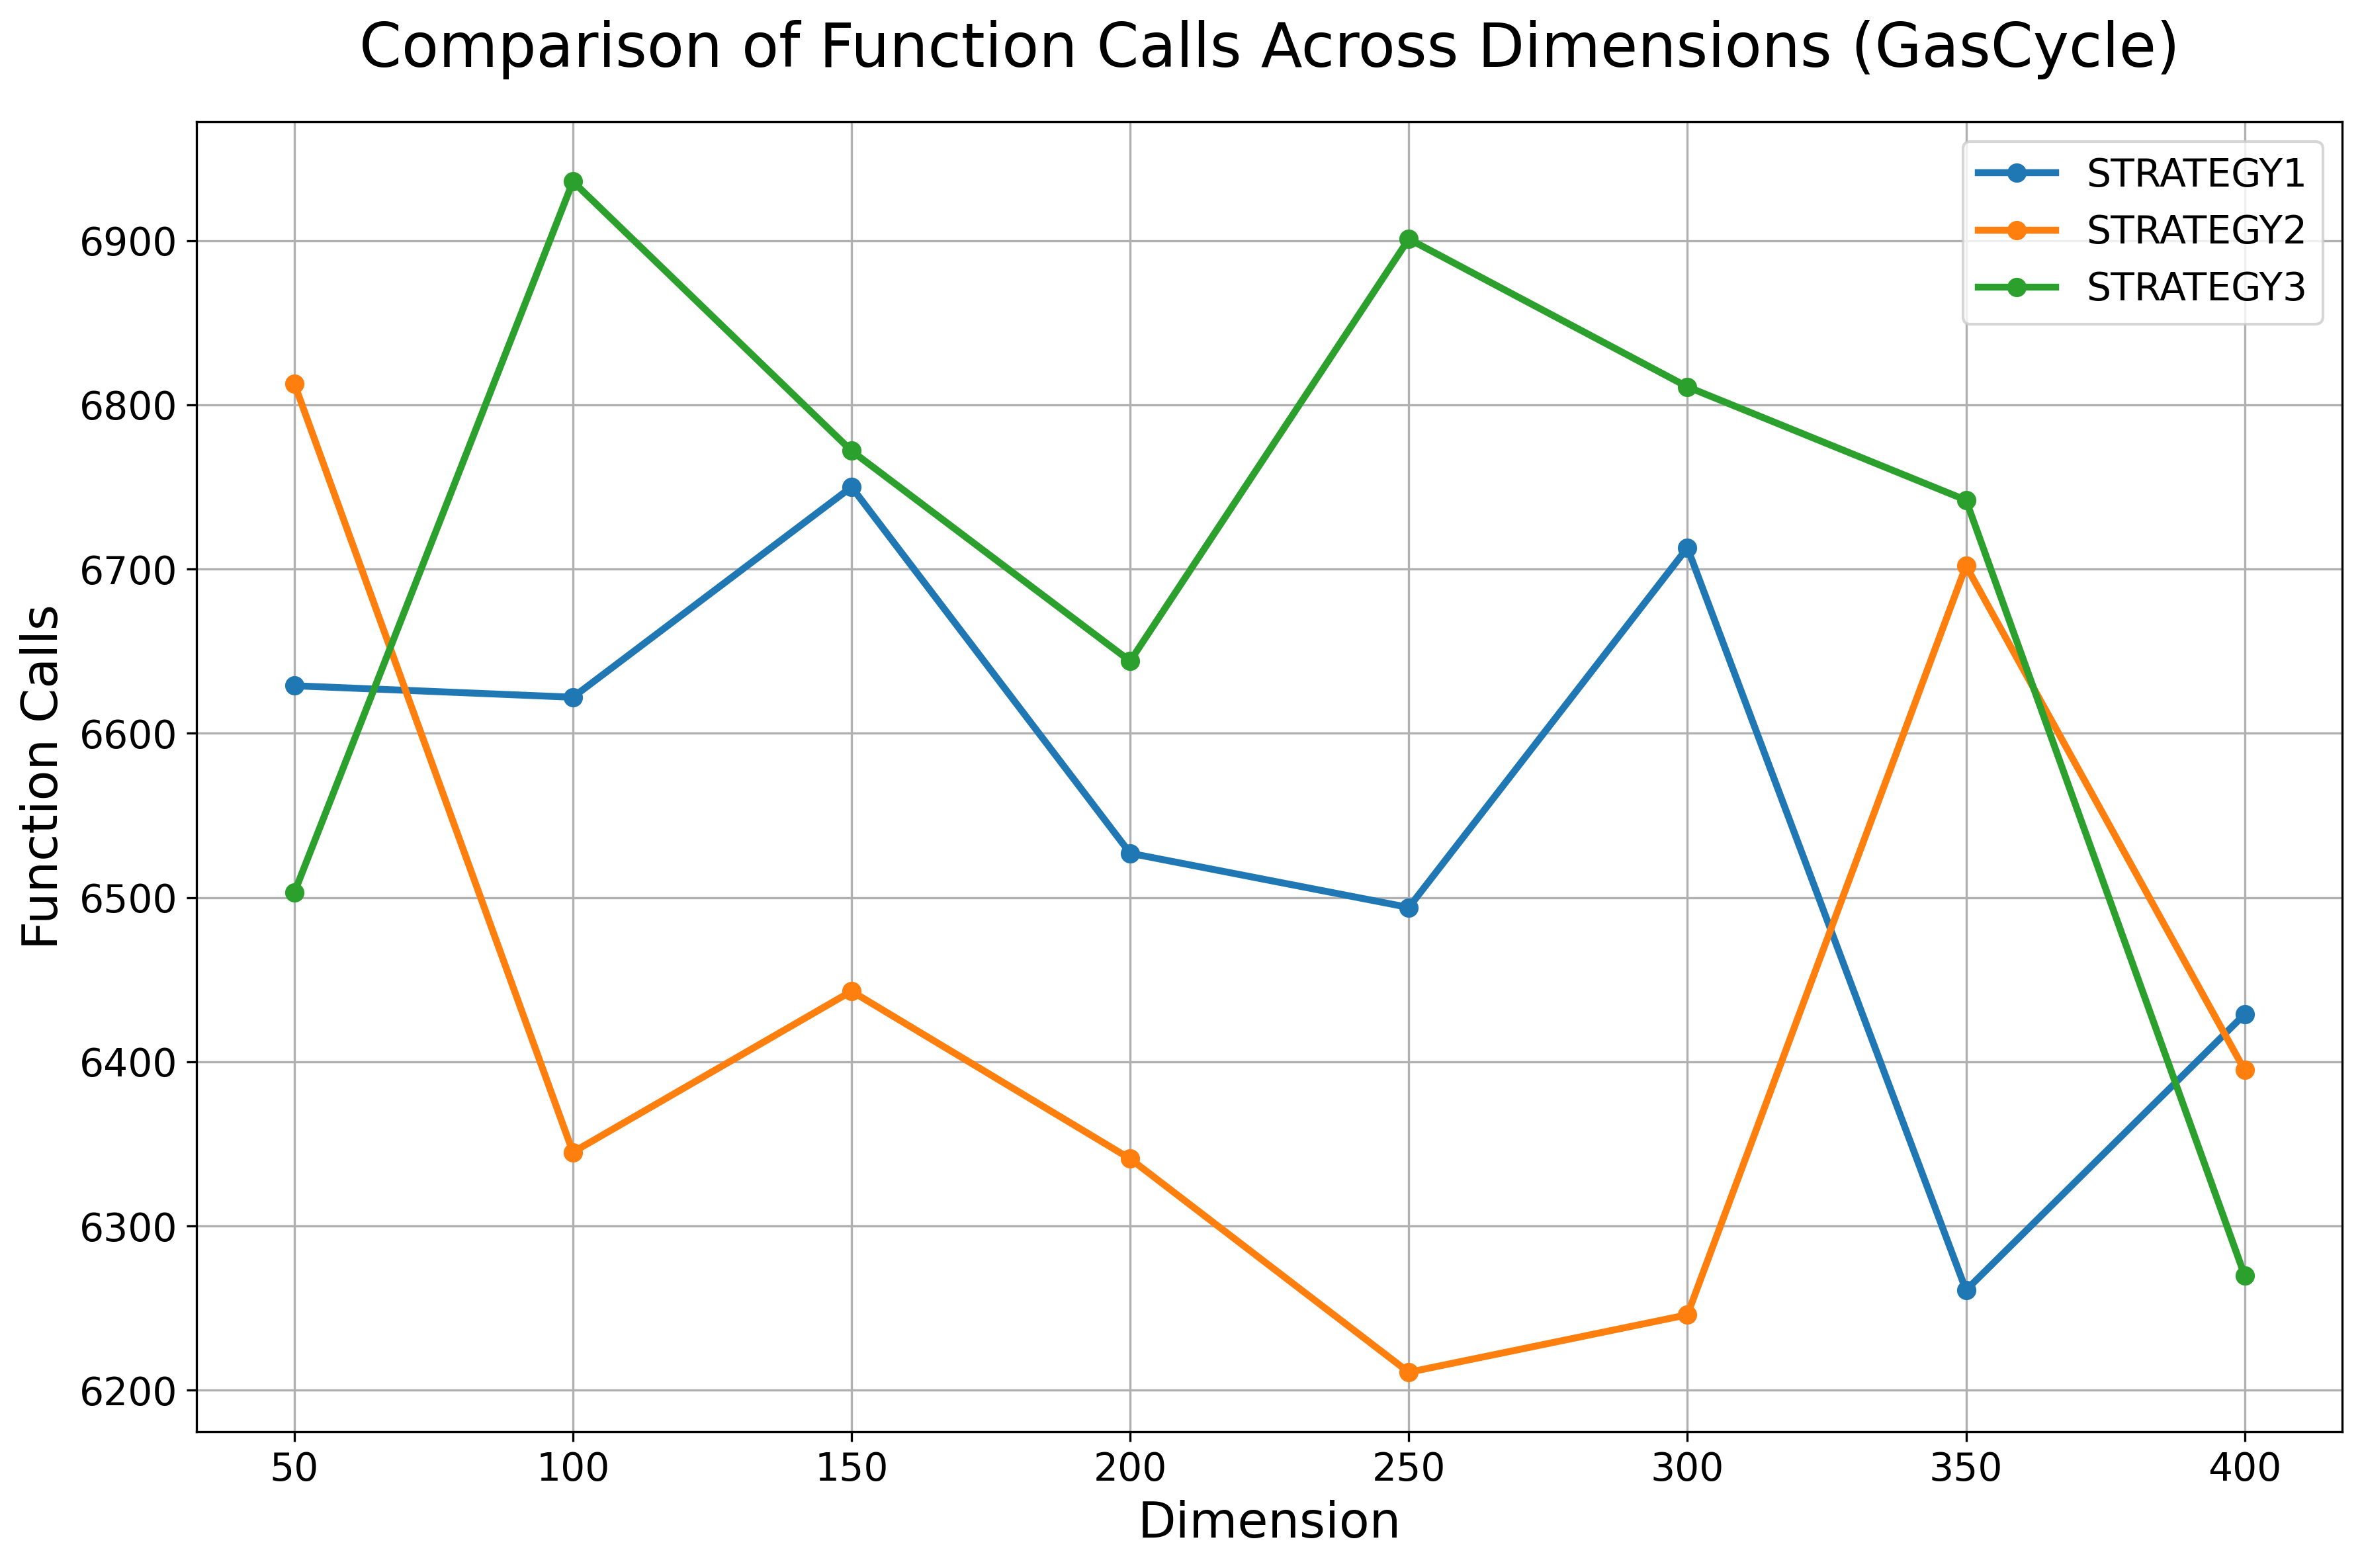
\includegraphics[scale=0.4]{GasCycle_Strategies}\caption{Communication Strategies on Practical Problems (GasCycle).\label{fig:Comparison-of-Function-2-1}}
\end{figure}

Figure \ref{fig:Comparison-of-Function-2-1-1} presents the comparison
of the number of objective function evaluations obtained by the three
communication strategies (STRATEGY1, STRATEGY2 and STRATEGY3) for
the LennardJones13 benchmark problem across different problem dimensions.
Lower values correspond to better optimization efficiency. The results
show that all three strategies exhibit very similar behavior, with
the number of function evaluations remaining relatively stable as
the dimensionality increases. STRATEGY2 achieves the lowest number
of evaluations in most dimensions, particularly at dimensions 50,
450 and 650 indicating a slightly lower computational cost. STRATEGY1
follows closely while STRATEGY3 generally requires a somewhat larger
number of function evaluations especially in the intermediate dimensions.
Overall, the differences among the three communication strategies
are relatively small suggesting that all of them provide robust and
consistent performance on the LennardJones13 problem. Nevertheless,
STRATEGY2 appears to offer a slight advantage in terms of convergence
efficiency achieving the lowest average number of function evaluations
across the examined dimensional range.

\begin{figure}[H]
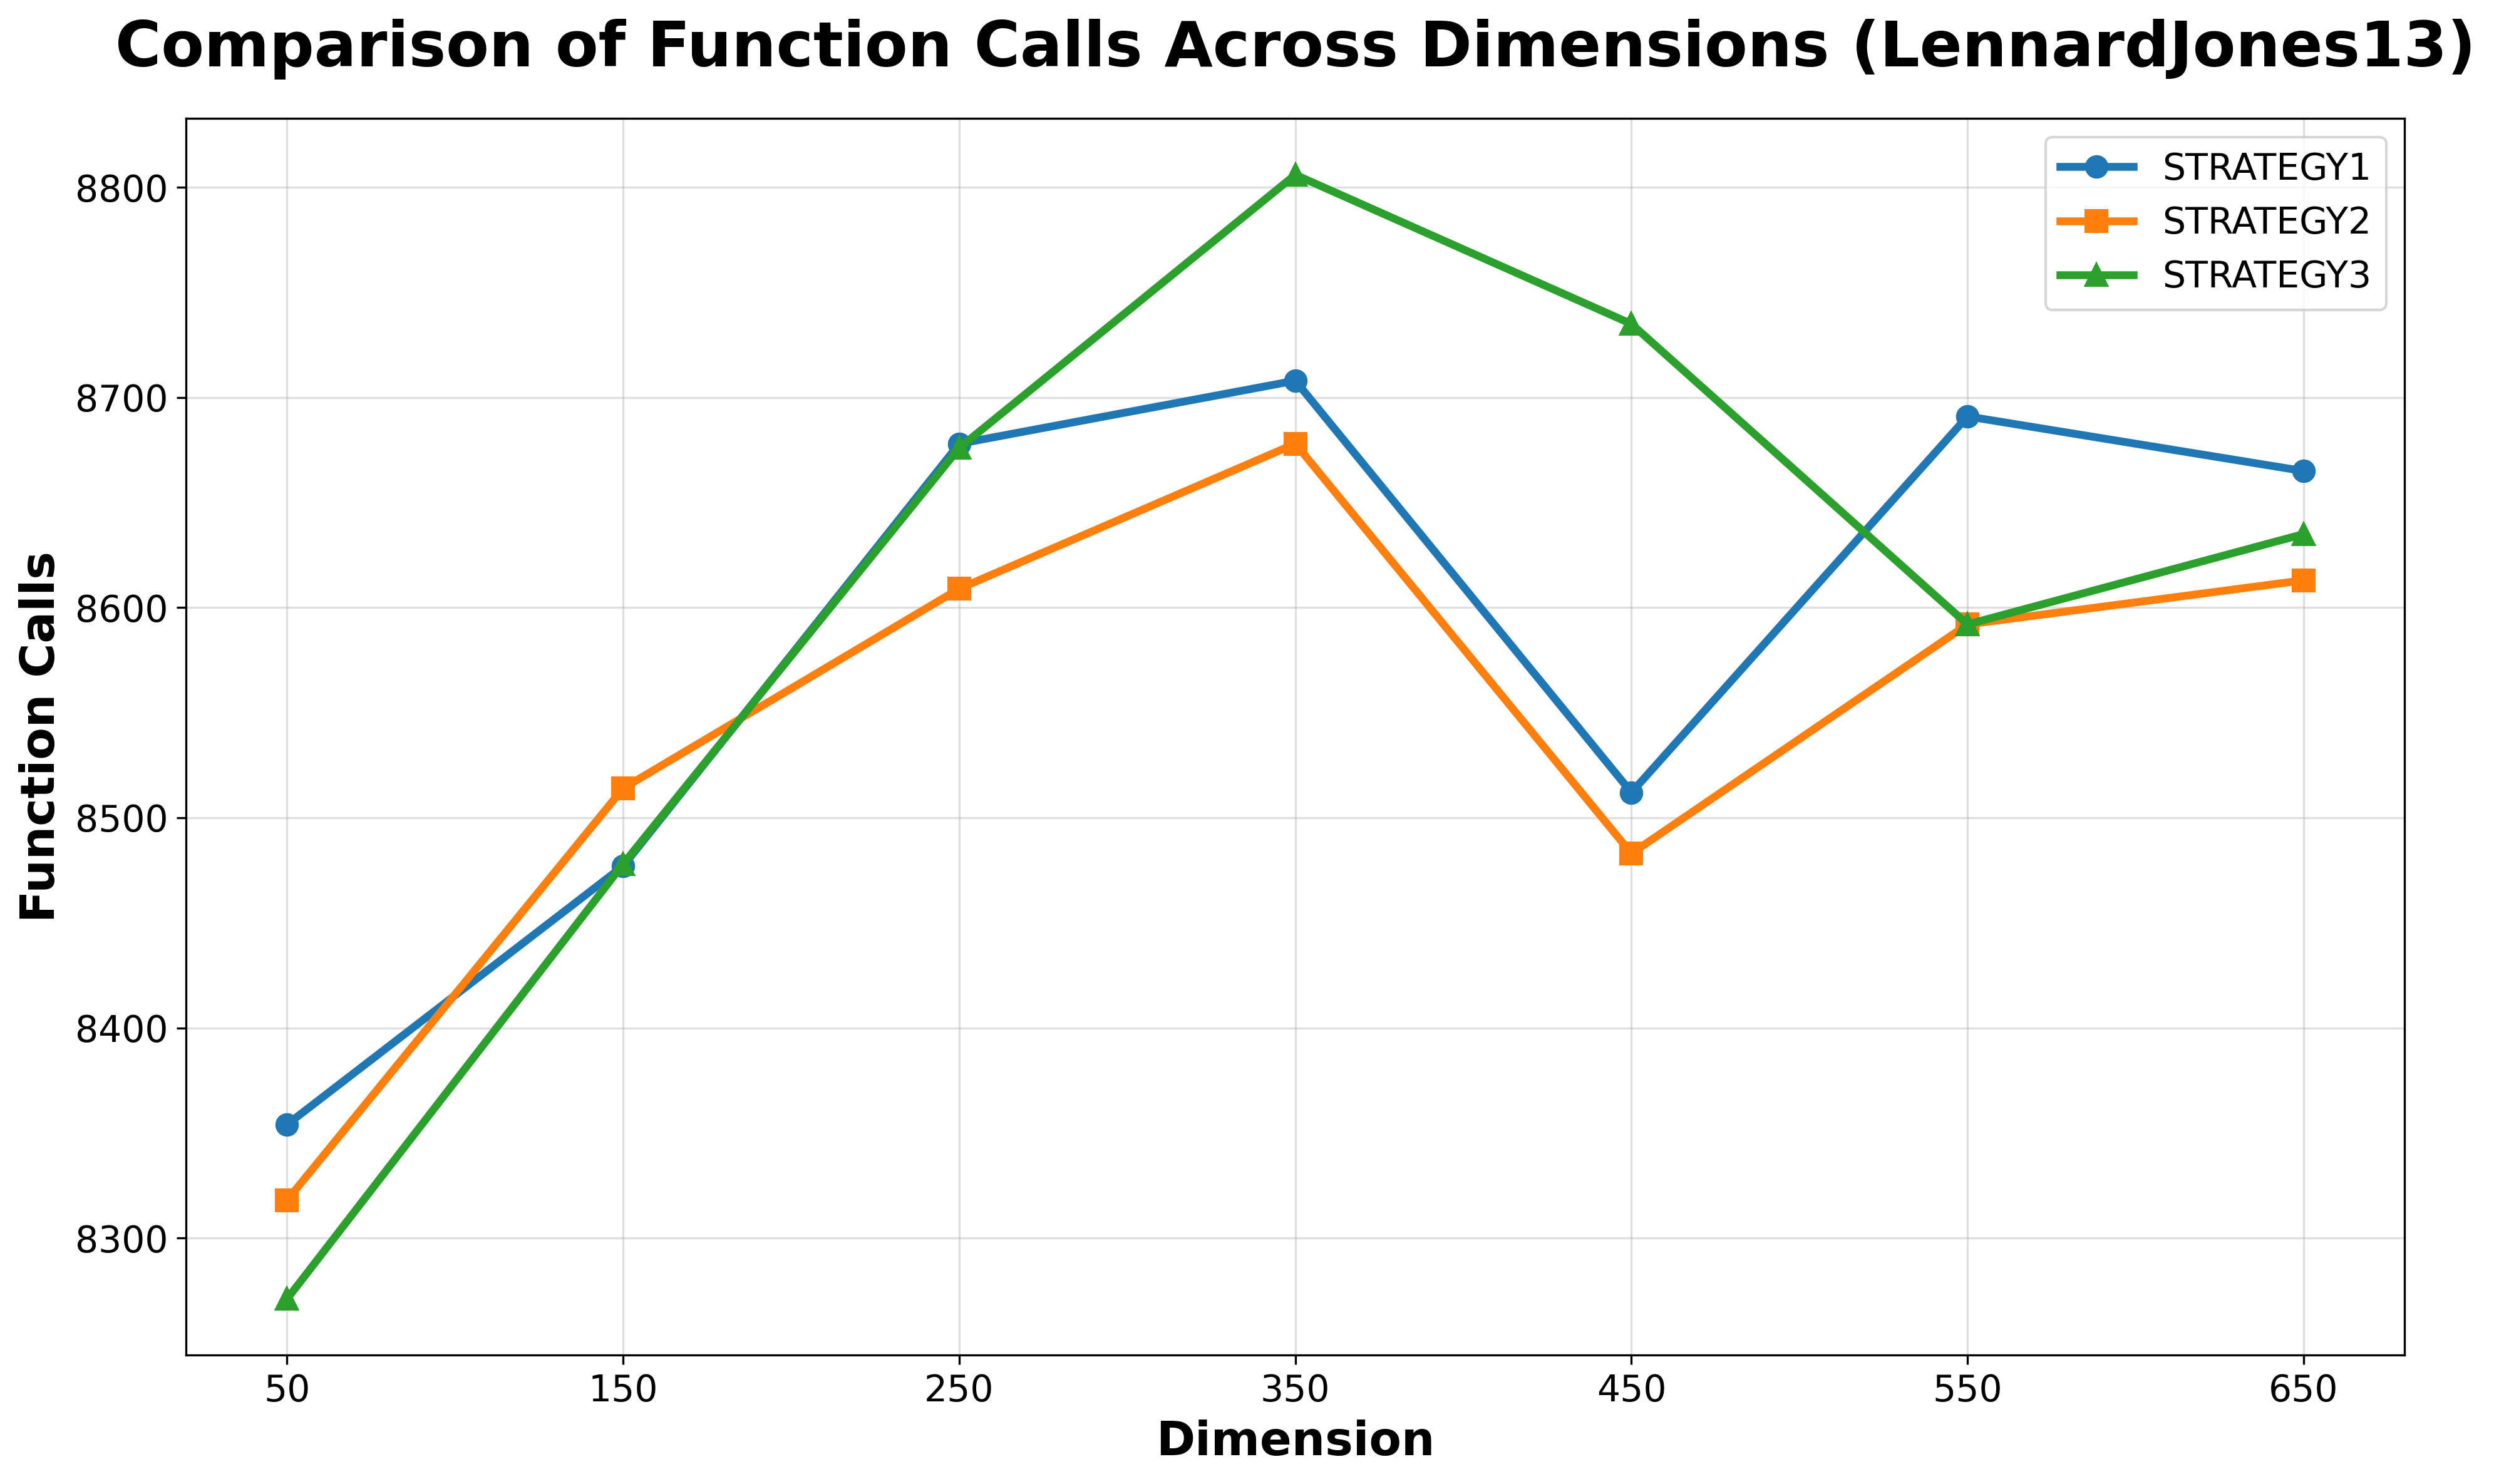
\includegraphics[scale=0.4]{LennardJones13_Strategies}\caption{Communication Strategies on Practical Problems (LennardJones13).\label{fig:Comparison-of-Function-2-1-1}}
\end{figure}


\section{Discussion\label{sec:Discussion}}

\subsection{Effect of the Cooperative Cluster Structure}

The experimental results demonstrate that the performance of the proposed
PEAO algorithm is strongly influenced by its cooperative parallel
structure. The incorporation of multiple clusters significantly improves
the search efficiency and convergence behavior of the algorithm. The
analysis of different numbers of clusters revealed that the search
performance depends on the population partitioning strategy. Configurations
employing 10 and 20 clusters achieved the lowest median number of
function evaluations while both smaller and larger numbers of clusters
resulted in reduced efficiency. These findings suggest the existence
of an optimal balance between population diversity and exploitation
capability. 

\subsection{Impact of the Propagation Mechanism}

The propagation mechanism proved to be a critical component of the
proposed framework. The comparison between the configurations with
and without propagation showed a substantial reduction in the number
of objective function evaluations when propagation was enabled. The
paired Wilcoxon test confirmed that this improvement is statistically
significant (p \textless{} 0.0001) indicating that information sharing
among clusters effectively accelerates convergence. The rapid dissemination
of high-quality solutions improves the global guidance of the search
process and contributes to a more efficient exploration of the search
space. Although propagation introduces additional communication overhead
the obtained results demonstrate that the benefits clearly outweigh
the associated cost.

\subsection{Analysis of Communication Strategies}

The communication strategy experiments demonstrated that the way information
is exchanged among clusters has a direct impact on optimization efficiency.
Among the examined strategies, the N-to-N communication scheme consistently
achieved the lowest computational cost, while the 1-to-1 strategy
required significantly more function evaluations. Statistical analysis
using the Friedman test confirmed the significance of these differences.
The superior performance of the N-to-N strategy suggests that extensive
information exchange enhances cooperation among clusters and facilitates
the rapid diffusion of promising solutions throughout the population.
Consequently, communication topology emerges as a key design factor
affecting the effectiveness of cooperative evolutionary search.

\subsection{Scalability on Practical Optimization Problems}

The practical optimization experiments on the GasCycle and LennardJones13
problems further validated the robustness of the proposed approach.
Across increasing problem dimensions, PEAO maintained stable behavior
in terms of both function evaluations and execution time. Although
some communication strategies exhibited small performance variations,
the overall trends remained consistent indicating good scalability
characteristics. These findings suggest that the proposed framework
can effectively handle increasing search-space complexity while maintaining
predictable computational requirements.

\subsection{Comparative Performance Evaluation}

The comparison with established metaheuristic algorithms showed that
PEAO achieves one of the lowest numbers of objective function evaluations
while maintaining competitive execution times. The Kruskal--Wallis
statistical tests confirmed that the observed differences are statistically
significant demonstrating the effectiveness of the proposed cooperative
search framework. The results indicate that the combination of adaptive
Cluster cooperation, efficient information propagation, and communication
mechanisms substantially enhances the optimization capability of PEAO.
Consequently, the proposed algorithm represents a robust and scalable
optimization approach capable of effectively addressing both benchmark
and practical optimization problems.

\subsection{Overall Assessment}

Overall, the findings demonstrate that the effectiveness of PEAO derives
from the synergistic interaction of its principal components, namely
population partitioning information propagation, and cooperative communication.
The experimental evidence consistently shows that these mechanisms
improve convergence efficiency reduce computational cost, and enhance
robustness. As a result, PEAO provides an efficient and scalable optimization
framework suitable for complex and high-dimensional optimization problems.

\section{Conclusions\label{sec:Conclusions}}

This work introduced the Parallel Enzyme Action Optimization (PEAO)
a cooperative population-based optimization framework designed to
enhance search efficiency through structured information exchange
and parallel exploration mechanisms. The proposed methodology combines
multiple interacting subpopulations with a communication mechanism
based on information propagation enabling the effective dissemination
of high-quality solutions while preserving population diversity throughout
the optimization process. The experimental results demonstrated that
both the information propagation mechanism and the communication mechanism
among subpopulations play a crucial role in determining the overall
performance of the algorithm. Efficient information sharing among
subpopulations accelerates convergence reduces computational cost
and enhances the stability of the search process. Furthermore, the
decomposition of the population into cooperating groups promotes a
more balanced exploration of the search space, reducing the risk of
premature convergence and increasing the likelihood of identifying
high-quality solutions. An additional contribution of this study is
the systematic investigation of different communication mechanisms
among subpopulations and alternative population configurations. The
findings reveal that the effectiveness of cooperative optimization
strongly depends on the manner in which subpopulations interact and
exchange information. Communication mechanisms that facilitate broader
knowledge dissemination consistently exhibit faster convergence improved
robustness and greater reliability throughout the search process.
These observations highlight cooperation and systematic knowledge
exchange as fundamental design principles for modern evolutionary
optimization algorithms. Overall, the proposed PEAO framework provides
an efficient, scalable and flexible optimization methodology capable
of addressing complex search spaces while maintaining an effective
balance between exploration and exploitation. The combination of cooperative
search propagation-driven knowledge transfer and adaptive population
organization establishes a solid foundation for solving computationally
demanding optimization problems.

Future research will focus on the development of self-adaptive communication
mechanisms, dynamic subpopulation management strategies and adaptive
propagation policies capable of automatically adjusting to the characteristics
of the optimization landscape. In addition, extending the framework
to constrained, dynamic and multi-objective optimization problems
represents a promising direction for further investigation. These
enhancements are expected to further strengthen the adaptability,
scalability and practical applicability of PEAO across a broader range
of real-world optimization challenges.

\vspace{6pt}


\authorcontributions{G.K., V.C. and I.G.T. conceived of the idea and the methodology,
and G.K. and V.C. implemented the corresponding software. G.K. conducted
the experiments, employing objective functions as test cases, and
the comparative experiments. I.G.T. performed the necessary statistical
tests. All authors have read and agreed to the published version of
the manuscript.}

\funding{This research has been financed by the European Union: Next Generation
EU project through the program Greece 2.0 National Recovery and Resilience
Plan, under the call RESEARCH--CREATE--INNOVATE; project name: “iCREW:
Intelligent small craft simulator for advanced crew training using
Virtual Reality techniques” (project code: TAEDK-06195).}

\institutionalreview{Not applicable.}

\informedconsent{Not applicable.}

\dataavailability{The original contributions presented in this study are included in
the article. Further inquiries can be directed to the corresponding
author.}

\conflictsofinterest{The authors declare no conflicts of interest.}

\appendix

\begin{adjustwidth}{-\extralength}{0cm}{}


\reftitle{References}
\begin{thebibliography}{999}
\bibitem[1]{DE_Large}Kyrou, G., Charilogis, V., \& Tsoulos, I. G.
(2026). A Novel Method That Is Based on Differential Evolution Suitable
for Large-Scale Optimization Problems. Foundations, 6(1), 2.

\bibitem[2]{Large1}Tang, K., Li, X., Suganthan, P. N., Yang, Z.,
\& Weise, T. (2007). Benchmark functions for the CEC’2010 special
session and competition on large-scale global optimization. Nature
inspired computation and applications laboratory, USTC, China, 24,
1-18.

\bibitem[3]{Large2}Li, X., Tang, K., Omidvar, M. N., Yang, Z., Qin,
K., \& China, H. (2013). Benchmark functions for the CEC 2013 special
session and competition on large-scale global optimization. gene,
7(33), 8.

\bibitem[4]{Large3}Molina, D., \& Herrera, F. (2015, May). Iterative
hybridization of DE with local search for the CEC'2015 special session
on large scale global optimization. In 2015 IEEE congress on evolutionary
computation (CEC) (pp. 1974-1978). IEEE.

\bibitem[5]{mechanical design}Mehta, P., Abderazek, H., Kumar, S.,
Sait, S. M., Yıldız, B. S., \& Yildiz, A. R. (2025). Comparative study
of state-of-the-art metaheuristics for solving constrained mechanical
design optimization problems: experimental analyses and performance
evaluations. Materials Testing, 67(2), 249-281.

\bibitem[6]{mechanical design-1}Mehta, P., Sait, S. M., Yildiz, B.
S., \& Yildiz, A. R. (2025). Enhanced hippopotamus optimization algorithm
and artificial neural network for mechanical component design. Materials
Testing, 67(4), 655-662.

\bibitem[7]{machine_learning_1}Bertsimas, D., \& Margaritis, G. (2025).
Global optimization: a machine learning approach. Journal of Global
Optimization, 91(1), 1-37.

\bibitem[8]{machine_learning_2}Gauthaman, S. A., Muniasamy, A., Kamaldheen,
R., Kumar, S. S. M., Murugesan, K., Viswanathan, M. K., \& Devendran,
H. (2026). Introduction to machine learning and optimization in healthcare.
In Integrative machine learning and optimization algorithms for disease
prediction (pp. 1-34). IGI Global Scientific Publishing.

\bibitem[9]{big data analysis}Theodorakopoulos, L., Karras, A., \&
Krimpas, G. A. (2025). Optimizing apache spark MLlib: Predictive performance
of large-scale models for big data analytics. Algorithms, 18(2), 74

\bibitem[10]{EAO-1}Rodan, A., Al-Tamimi, A. K., Al-Alnemer, L., Mirjalili,
S., \& Tiňo, P. (2025). Enzyme action optimizer: a novel bio-inspired
optimization algorithm: A. Rodan et al. The Journal of Supercomputing,
81(5), 686.

\bibitem[11]{EAO1.}Cinar, R. F. (2025). Enzyme action optimizer based
infinite impulse response filter identification through a comprehensive
benchmark across full and reduced orders. Scientific Reports.

\bibitem[12]{EAO2.}Turkeri, C., Ekinci, S., Yüksek, G., \& Li, D.
(2025). A Modified Enzyme Action Optimizer-Based FOPID Controller
for Temperature Regulation of a Nonlinear Continuous Stirred Tank
Reactor. Fractal and Fractional, 9(12), 811.

\bibitem[13]{EAO3}Hegazy, A. E., Makhlouf, M. A., Salem, O. A., \&
Hafiz, B. (2026). Improving predictive accuracy in medical datasets
using enhanced enzyme action optimizer for feature selection: AE Hegazy
et al. The Journal of Supercomputing, 82(2), 84.

\bibitem[14]{EAO5}Ekinci, S., Izci, D., Jabari, M., Bajaj, M., \&
Rubanenko, O. (2025). Design of a novel and robust 2-DOF PIDA controller
based on enzyme action optimizer for ball position regulation in magnetic
levitation systems. Scientific Reports, 15(1), 29360.

\bibitem[15]{EAO4-1}Izci, D., Ekinci, S., Cinar, R. F., Yuksek, G.,
Rashdan, M., \& Salman, M. (2025, September). Parameter Identification
In Nonlinear Systems Using Enzyme Action Optimizer. In 2025 Innovations
in Intelligent Systems and Applications Conference (ASYU) (pp. 1-4).
IEEE.

\bibitem[16]{EAO4}Ekinci, S., Izci, D., Yuksek, G., Cinar, R. F.,
Rashdan, M., \& Salman, M. (2025, September). Dynamic Enzyme Action
Optimizer (DEAO): An Adaptive Bio-Inspired Approach for Classical
Benchmark Functions. In 2025 Innovations in Intelligent Systems and
Applications Conference (ASYU) (pp. 1-5). IEEE.

\bibitem[17]{PEAO}Li, H., Govindarajan, V., Ang, T. F., Ayadi, M.,
Ku, C. S., Leong, M. C., ... \& Por, L. Y. (2026). PEAO: a bio-inspired
parallel optimizer with a multi-strategy communication mechanism for
breast cancer diagnosis. Scientific Reports.

\bibitem[18]{BFGS}Powell, M. J. D. (1989). A tolerant algorithm for
linearly constrained optimization calculations. Mathematical Programming,
45(1), 547-566.

\bibitem[19]{stopping_rule}Charilogis, V., \& Tsoulos, I. G. (2022).
Toward an ideal particle swarm optimizer for multidimensional functions.
Information, 13(5), 217.

\bibitem[20]{test_function}Ali, M. M., \& Kaelo, P. (2008). Improved
particle swarm algorithms for global optimization. Applied mathematics
and computation, 196(2), 578-593.

\bibitem[21]{test_function-1}Koyuncu, H., \& Ceylan, R. (2019). A
PSO based approach: Scout particle swarm algorithm for continuous
global optimization problems. Journal of Computational Design and
Engineering, 6(2), 129-142.

\bibitem[22]{test_function2}Siarry, P., Berthiau, G., Durdin, F.,
\& Haussy, J. (1997). Enhanced simulated annealing for globally minimizing
functions of many-continuous variables. ACM Transactions on Mathematical
Software (TOMS), 23(2), 209-228.

\bibitem[23]{test_function3}LaTorre, A., Molina, D., Osaba, E., Poyatos,
J., Del Ser, J., \& Herrera, F. (2021). A prescription of methodological
guidelines for comparing bio-inspired optimization algorithms. Swarm
and Evolutionary Computation, 67, 100973.

\bibitem[24]{OPTIMUS}Tsoulos, I. G., Charilogis, V., Kyrou, G., Stavrou,
V. N., \& Tzallas, A. (2025). OPTIMUS: A Multidimensional Global Optimization
Package. Journal of Open Source Software, 10(108), 7584.

\bibitem[25]{Genetic}Wan, H. (2026). Applying the genetic algorithm
to optimization problems. WIT Transactions on Information and Communication
Technologies, 2.

\bibitem[26]{Genetic-1}Pereira, C. M. N. A., Schirru, R., \& Martinez,
A. S. (2026). Learning an optimized classification system from a data
base of time series patterns using genetic algorithms. WIT Transactions
on Information and Communication Technologies, 22.

\bibitem[27]{DE}Koyuncuoğlu, M. U. (2026). Sustainable configuration
of production lines: Multi-objective energy-efficient optimization
with adaptive differential evolution and golden ratio algorithms. Engineering
Applications of Artificial Intelligence, 165, 113469.

\bibitem[28]{DE1}Horrillo-Quintero, P., Garcia-Trivino, P., Carrasco-Gonzalez,
D., \& Fernandez-Ramirez, L. M. (2026). Optimal control strategy based
on differential evolution algorithm for seamless transition between
islanded and grid-connected operation modes in microgrid clusters. Expert
Systems with Applications, 297, 129461.

\bibitem[29]{GWO}Long, W., Jiao, J., Liang, X., \& Tang, M. (2018).
Inspired grey wolf optimizer for solving large-scale function optimization
problems. Applied Mathematical Modelling, 60, 112-126.

\bibitem[30]{GWO1}Long, W., Cai, S., Jiao, J., \& Tang, M. (2020).
An efficient and robust grey wolf optimizer algorithm for large-scale
numerical optimization: W. Long et al. Soft Computing, 24(2), 997-1026.

\bibitem[31]{PARALLELDE}Charilogis, V., \& Tsoulos, I. G. (2023).
A parallel implementation of the differential evolution method. Analytics,
2(1), 17-30.

\bibitem[32]{PARALLELDE-1}Tasoulis, D. K., Pavlidis, N. G., Plagianakos,
V. P., \& Vrahatis, M. N. (2004, June). Parallel differential evolution.
In IEEE Congress on Evolutionary Computation (pp. 2023-2029).

\bibitem[33]{SAOP}Kyrou, G., Tsoulos, I. G., Gianni, A. M., \& Charilogis,
V. (2025). Parallel smell agent optimization (SAO): collaborative
subpopulations for accelerated convergence. Symmetry, 17(4), 592.

\bibitem[34]{BGWO1}Adhikary, J., \& Acharyya, S. (2022). Randomized
Balanced Grey Wolf Optimizer (RBGWO) for solving real life optimization
problems. Applied Soft Computing, 117, 108429.

\bibitem[35]{BGWO2}Wang, J., Lin, D., Zhang, Y., \& Huang, S. (2022).
An adaptively balanced grey wolf optimization algorithm for feature
selection on high-dimensional classification. Engineering Applications
of Artificial Intelligence, 114, 105088.

\bibitem[36]{woa}Almufti, S. M., Hassan, N. S., Mercado, M. C., Felix,
J. W. G., Barbosa, T. S., \& Supan, F. E. (2026). Survey on whale
optimization algorithm: from fundamental principles to modern adaptations
and applications.

\bibitem[37]{Woa1}Su, Y., \& Liu, Y. (2026). A novel marine predator
whale optimization algorithm for global numerical optimization. Engineering
Optimization, 58(1), 203-239.

\bibitem[38]{GasCycle}Luo, B., Su, X., Zhang, S., Yan, P., Liu, J.,
\& Li, R. (2025). Analysis of a novel gas cycle cooler with large
temperature glide for space cooling. Energy, 326, 136294.

\bibitem[39]{Lennard}Locatelli, M., \& Schoen, F. (2002). Fast global
optimization of difficult Lennard-Jones clusters. Computational Optimization
and Applications, 21(1), 55-70.

\bibitem[40]{Lennard-1}Wang, X., Ramírez-Hinestrosa, S., Dobnikar,
J., \& Frenkel, D. (2020). The Lennard-Jones potential: when (not)
to use it. Physical Chemistry Chemical Physics, 22(19), 10624-10633.

\end{thebibliography}
%%%%%%%%%%%%%%%%%%%%%%%%%%%%%%%%%%%%%%%%%%
%% for journal Sci
%\reviewreports{\\
%Reviewer 1 comments and authors' response\\
%Reviewer 2 comments and authors' response\\
%Reviewer 3 comments and authors' response
%}
%%%%%%%%%%%%%%%%%%%%%%%%%%%%%%%%%%%%%%%%%%

\PublishersNote{}

\end{adjustwidth}{}
\end{document}
